% ThinkAlgo — Đại số và Phương trình — Lớp 7
% Edition: teacher (with solutions), VI.  Generated by build_grade7.py — edit body/ and rebuild.
\documentclass[11pt]{article}
\newif\ifsol \soltrue
\usepackage{iftex}
\ifPDFTeX
  \usepackage[utf8]{inputenc}\usepackage[T5]{fontenc}
\else
  \usepackage{fontspec}
\fi
\usepackage[a4paper,top=2.95cm,headheight=1.5cm,headsep=0.45cm,bottom=3.1cm,left=1.9cm,right=1.9cm]{geometry}
\usepackage{amsmath,amssymb}
\usepackage{tikz}\usetikzlibrary{calc,shadows,shapes.geometric}
\usepackage[most]{tcolorbox}
\usepackage{enumitem}
\usepackage{array}
\usepackage{tabularx}
\usepackage{colortbl}
\usepackage{comment}
\usepackage{needspace}
\usepackage{fancyhdr}
\usepackage{fontawesome5}
\usepackage{graphicx}
\usepackage{microtype}
% PDF outline (bookmarks) so each chapter shows in the reader's outline — does not change the page layout
\usepackage[hidelinks,unicode,bookmarksnumbered=false,bookmarksopen=true,bookmarksopenlevel=0]{hyperref}
\usepackage{bookmark}
\usetikzlibrary{decorations.pathreplacing,arrows.meta,angles,quotes,patterns,positioning,through,intersections}

% ---------------- palette: navy family + subtle light tint; orange ONLY in the logo ----------------
% ----- EXACT palette from the user's original main (36).tex (vivid, not pale) -----
\definecolor{tmBlue}{RGB}{66,133,244}   % problem / header / section
\definecolor{tmGreen}{RGB}{52,168,83}   % solution
\definecolor{tmOrange}{RGB}{255,152,0}  % example
\colorlet{Navy}{tmBlue}                 % header rule / section heading / badge / divider
\definecolor{NavyD}{HTML}{222222}       % solution body text (dark, readable)
\colorlet{Gold}{Navy}
\colorlet{ProbBlue}{tmBlue}             % problem boxes
\colorlet{SolGreen}{tmGreen}            % solution boxes
\definecolor{AnsRed}{HTML}{E02424}      % vivid red for answers / totals
\definecolor{CardGreen}{HTML}{34A853}   % digit-card green
\definecolor{StarGold}{HTML}{F2B134}    % difficulty star (gold)
\definecolor{KidOrange}{HTML}{DE8A2C}   % logo accent only
\definecolor{Ink}{HTML}{1F2733}       % body text
\definecolor{Slate}{HTML}{5B6A82}     % muted labels
\definecolor{Line}{HTML}{C6D0DF}      % light hairlines / student boxes
\definecolor{Tint}{HTML}{EDF1F7}      % pale panel fill (worked solution / answer)
% aliases so older names keep working
\colorlet{TextDark}{Ink}\colorlet{TextGray}{Slate}\colorlet{Soft}{Slate}
\colorlet{CardLine}{Line}\colorlet{Teal}{Navy}\colorlet{ProbB}{Navy}\colorlet{SolG}{Navy}
% bright, kid-friendly colours for bar-model (sơ đồ đoạn thẳng) blocks
\definecolor{tmPurple}{RGB}{124,77,226}
\definecolor{tmTeal}{RGB}{0,150,136}
\definecolor{tmPink}{RGB}{233,30,99}
\AtBeginDocument{\color{Ink}}
\raggedbottom  % natural flow, even spacing (no stretched gaps)
\setlength{\parindent}{0pt}\setlength{\parskip}{0.18em}
\renewcommand{\arraystretch}{1.35}
\providecommand{\AnsWord}{Đáp số}

% ---------------- brand logo (original mark) ----------------
\newcommand{\logomark}[1]{\begin{tikzpicture}[baseline=-0.55ex,scale=#1]
  \draw[KidOrange,line width=1.5pt] (-0.27,0) .. controls (-0.27,0.23) and (0,0.23) .. (0,0)
        .. controls (0,-0.23) and (-0.27,-0.23) .. (-0.27,0);
  \draw[Navy,line width=1.5pt] (0.27,0) .. controls (0.27,0.23) and (0,0.23) .. (0,0)
        .. controls (0,-0.23) and (0.27,-0.23) .. (0.27,0);
\end{tikzpicture}}
% real brand logo image (gold infinity + "think algo" wordmark)
\newcommand{\logohead}{\IfFileExists{logo.png}{\includegraphics[height=1.35cm]{logo.png}}%
  {\raisebox{0.35cm}{\logomark{1.5}\hspace{0.5em}{\Large\bfseries\color{KidOrange}think\,\color{Navy}algo}}}}

% ---------------- running header (logo + Name/Date + topic) on EVERY page, single navy rule ----------------
\pagestyle{fancy}\fancyhf{}
\renewcommand{\headrulewidth}{1.4pt}\renewcommand{\footrulewidth}{0pt}
\renewcommand{\headrule}{{\color{Navy}\hrule height 1.3pt}}
\fancyhead[L]{\raisebox{-0.95cm}{\logohead}}
\fancyhead[R]{\setlength{\tabcolsep}{0pt}%
  \begin{tabular}{@{}r@{}}
    {\small\color{Ink}{\color{tmBlue}\faUserEdit}~\NameWord:~\rule{3.0cm}{0.5pt}\quad{\color{tmBlue}\faCalendarDay}~\DateWord:~\rule{1.9cm}{0.5pt}}\\[5pt]
    {\large\bfseries\color{Navy}\CurTopic}
  \end{tabular}}

% ---------------- footer (rounded page border + Topic/Grade + thinkalgo.com + page + tagline) ----------------
% NOTE: a remember-picture overlay must be placed DIRECTLY in \fancyfoot, NOT inside \def/\newcommand.
\fancyfoot[C]{\begin{tikzpicture}[remember picture, overlay]
  \draw[Navy!40, line width=1.4pt, rounded corners=12pt]
     ($(current page.north west)+(0.8cm,-0.8cm)$) rectangle ($(current page.south east)+(-0.8cm,0.45cm)$);
  \coordinate (FL) at ($(current page.south west)+(1.2cm, 2.18cm)$);
  \coordinate (FR) at ($(current page.south east)+(-1.2cm, 2.18cm)$);
  \draw[Navy!55, line width=1pt] (FL) -- (FR);
  \node[fill=white, draw=Navy, line width=1.2pt, rounded corners=8pt, font=\bfseries\small,
        text=Navy, inner xsep=11pt, inner ysep=4pt] at ($(current page.south)+(0,2.18cm)$) {{\color{tmBlue}\faGlobe}\ \ thinkalgo.com};
  \node[text=Slate, font=\footnotesize, anchor=north west, align=left, inner sep=0pt, text width=7.6cm]
        at ($(FL)+(0.1cm,-0.30cm)$) {{\color{tmBlue}\faTag}\ \TopicWord: \textbf{\color{Ink}\CurTopic}\\[1.5pt]{\color{tmBlue}\faGraduationCap}\ \DocGrade};
  \node[text=Slate, font=\footnotesize] at ($(current page.south)+(0,1.20cm)$) {\thepage};
  \node[text=Slate, font=\scriptsize, anchor=north east, align=right, inner sep=0pt, text width=7.4cm]
        at ($(FR)+(-0.1cm,-0.34cm)$) {{\normalsize\bfseries\color{Navy}ThinkAlgo}\ — From Math Thinking to Code};
\end{tikzpicture}}

% ---------------- page-1 lead-in (topic is already in the header; keep a slim spacer) ----------------
\newcommand{\titlehead}{\vspace*{-0.2cm}}
\providecommand{\CurTopic}{}

% chapter banner + sets the running-header topic. #1 = number, #2 = title
\newcommand{\chapterhead}[2]{\renewcommand{\CurTopic}{#2}%
  \setcounter{seccnt}{0}% each chapter is independent: section badges restart at 1
  \phantomsection\pdfbookmark[0]{#1. #2}{chap#1}\label{chap:#1}% add this chapter to the PDF outline + TOC ref
  \par\vspace{0.1cm}\noindent\begin{tikzpicture}[baseline=-0.5ex]
    \node[circle,fill=tmBlue,text=white,font=\Large\bfseries,minimum size=0.95cm,inner sep=0pt](cn){#1};
    \node[anchor=west,font=\LARGE\bfseries,text=tmBlue] at ([xshift=12pt]cn.east){#2};
  \end{tikzpicture}\par\vspace{4pt}\noindent\textcolor{tmBlue}{\rule{\linewidth}{2pt}}\par\vspace{0.5cm}}

% ---------------- section heading (outline navy number badge, no fill) ----------------
\newcounter{seccnt}
\newcommand{\shead}[1]{\par\vspace{0.7em}\refstepcounter{seccnt}%
  \noindent
\begin{tikzpicture}[baseline=-0.6ex]
    \node[circle,draw=Gold,line width=1.2pt,text=Gold,font=\bfseries,minimum size=1.05em,inner sep=1pt]{\theseccnt};
  \end{tikzpicture}\hspace{0.4em}{\large\bfseries\color{Navy} #1}\par\vspace{0.25em}}

% ============ boxes EXACTLY per the original main (36).tex: solid-blue PROBLEM, solid-orange EXAMPLE,
%              outline-green SOLUTION, all with drop shadow + rounded corners ============
% ---------------- knowledge box: white, tmBlue border + left accent + drop shadow ----------------
\newtcolorbox{knowbox}{enhanced,breakable,colback=white,colframe=tmBlue!70,boxrule=0.9pt,arc=5pt,
  left=12pt,right=11pt,top=6pt,bottom=6pt,drop shadow,
  borderline west={3.5pt}{0pt}{tmBlue}}

% ---------------- EXAMPLE (Ví dụ): SOLID ORANGE tab, white text ----------------
\newtcolorbox{exbox}[1]{enhanced,breakable,colback=white,colframe=tmOrange,boxrule=1pt,arc=5pt,
  left=12pt,right=11pt,top=14pt,bottom=7pt,drop shadow,
  attach boxed title to top left={xshift=10pt,yshift=-\tcboxedtitleheight/2},
  boxed title style={colback=tmOrange,colframe=tmOrange,arc=4pt,boxrule=0pt,drop shadow},
  title={#1},fonttitle=\bfseries\color{white}}
\newcommand{\guide}{\par\vspace{2pt}{\bfseries\color{tmBlue}\GuideWord}\par\nopagebreak}

% ---------------- PROBLEM (Bài): SOLID BLUE tab, white text ----------------
\newtcolorbox{probbox}[2]{enhanced,breakable,colback=white,colframe=tmBlue,boxrule=1pt,arc=5pt,
  left=12pt,right=10pt,top=14pt,bottom=7pt,drop shadow,
  attach boxed title to top left={xshift=10pt,yshift=-\tcboxedtitleheight/2},
  boxed title style={colback=tmBlue,colframe=tmBlue,arc=4pt,boxrule=0pt,drop shadow},
  fonttitle=\bfseries\color{white},title={\ProbWord\ #1\ifx\relax#2\relax\else#2\fi}}

% ---------------- SOLUTION (Lời giải): OUTLINE GREEN tab (white fill, green border + text) ----------------
% Teacher: a green tcolorbox. Student: the body is dropped entirely (comment pkg — robust with tables/\\).
\ifsol
  \newtcolorbox{solbox}{enhanced,breakable,colback=white,colframe=tmGreen,boxrule=1pt,arc=5pt,
    left=12pt,right=10pt,top=14pt,bottom=7pt,drop shadow,
    attach boxed title to top left={xshift=10pt,yshift=-\tcboxedtitleheight/2},
    boxed title style={colback=white,colframe=tmGreen,boxrule=1pt,arc=4pt,drop shadow},
    fonttitle=\bfseries\color{tmGreen!88!black},title={\SolTitle},before upper={\color{NavyD}}}
\else
  \excludecomment{solbox}
\fi

% ---------------- answer highlight: label green, value RED ----------------
\newcommand{\ans}[1]{\par\smallskip{\bfseries\color{tmGreen!88!black}\AnsWord:}\ {\bfseries\color{AnsRed}#1}\par}

% ---------------- digit cards (exact original style: fill=c!10, border=c!60!black, drop shadow) ----------------
% \digitcards{0/gray,1/cyan,2/green,3/cyan} : value/colour pairs
\newcommand{\digitcards}[1]{\begin{center}\begin{tikzpicture}[scale=0.7,transform shape,font=\sffamily]
  \def\dx{0}\foreach \v/\c in {#1}{
    \node[draw=\c!60!black,line width=1.5pt,fill=\c!10,rounded corners=4pt,
          minimum width=1cm,minimum height=1.4cm,drop shadow] at (\dx,0){\Huge\bfseries \v};
    \pgfmathsetmacro\dx{\dx+1.5}\xdef\dx{\dx}}
\end{tikzpicture}\end{center}}

% ---------------- student working space (white, light border) ----------------
\newcommand{\worksp}[1]{\ifsol\else\begin{tcolorbox}[colback=white,colframe=Line,boxrule=0.8pt,
  arc=5pt,height=\dimexpr#1+0.05cm\relax,left=8pt,right=8pt,top=4pt,bottom=4pt]{\footnotesize\color{Slate}\itshape\WorkWord}\end{tcolorbox}\fi}

% ---------------- \probsol{solution} : Teacher shows the green solution box; Student shows a BLANK
%   "Bài làm" box whose height matches that solution's height (writing room = work needed), so both
%   versions have identical per-problem height and paginate the same. ----------------
\newsavebox{\solmeasure}\newlength{\solht}
\newcommand{\probsol}[1]{%
  \begin{lrbox}{\solmeasure}\begin{minipage}{\dimexpr\linewidth-24pt\relax}#1\end{minipage}\end{lrbox}%
  \ifsol
    \begin{solbox}#1\end{solbox}%
  \else
    \setlength{\solht}{\dimexpr\ht\solmeasure+\dp\solmeasure+0.85cm\relax}%
    \ifdim\solht<1.35cm\setlength{\solht}{1.35cm}\fi
    \ifdim\solht>\StudentMaxWork\setlength{\solht}{\StudentMaxWork}\fi
    \begin{tcolorbox}[colback=white,colframe=Line,boxrule=0.8pt,arc=5pt,
      left=8pt,right=8pt,top=4pt,bottom=4pt,height=\solht]{\footnotesize\color{Slate}\itshape\WorkWord}\end{tcolorbox}%
  \fi}

% ---------------- practice divider: blue left accent bar, no fill ----------------
\newcommand{\dividerbar}[1]{\par\vspace{0.6em}\noindent
  \begin{tcolorbox}[enhanced,frame hidden,interior hidden,borderline west={5pt}{0pt}{ProbBlue},
    colback=white,left=12pt,right=12pt,top=5pt,bottom=5pt,arc=4pt]
  {\large\bfseries\color{ProbBlue} #1}\end{tcolorbox}\vspace{0.4em}}

% place-value choice-count diagram (Cambridge style): #1 = "label/count/note/color" list, #2 = result
% notes must NOT contain commas or slashes (they separate \foreach fields)
\newcommand{\countboxes}[2]{\begin{center}\begin{tikzpicture}[scale=0.62,transform shape,font=\sffamily]
  \def\xx{0}%
  \foreach \lab/\cnt/\note/\col [count=\i] in {#1}{%
    \ifnum\i>1\relax \node[text=gray,font=\Huge] at (\xx-1.8,0){$\times$};\fi
    \node[draw=\col!65,fill=\col!8,rounded corners=3pt,line width=1pt,minimum width=2.7cm,minimum height=1.7cm] at (\xx,0){};
    \node[text=\col!85,font=\bfseries] at (\xx,0.58){\lab};
    \node[text=\col!88,font=\Huge\bfseries] at (\xx,-0.1){\cnt};
    \node[text=gray,font=\scriptsize] at (\xx,-1.05){\note};
    \pgfmathsetmacro\xx{\xx+3.6}\xdef\xx{\xx}}%
  \node[text=gray,font=\Huge] at (\xx-1.8,0){$=$};
  \node[text=red,font=\Huge\bfseries] at (\xx,0){#2};
\end{tikzpicture}\end{center}}

% ======== bar model (sơ đồ đoạn thẳng): lightly-rounded blocks, darker border, tiny gaps, bright colours ========
% one block: \blk{x1}{x2}{yc}{height}{colour}{label}  (a small gap is left on each side)
\newcommand{\blk}[6]{%
  \draw[rounded corners=1.3pt,fill=#5!16,draw=#5!80!black,line width=1pt]
    (#1+0.045,#3-#4/2) rectangle (#2-0.045,#3+#4/2);
  \node[font=\small\bfseries,text=#5!52!black] at ({(#1+#2)/2},#3){#6};}
% measurement with a double-headed ARROW (not a brace) + label above the span: \brcup{x1}{x2}{y}{label}
\newcommand{\brcup}[4]{%
  \draw[<->,>=stealth,tmBlue!72!black,line width=0.7pt] (#1+0.05,#3)--(#2-0.05,#3);
  \node[above=-1.5pt,font=\footnotesize,text=tmBlue!58!black] at ({(#1+#2)/2},#3){#4};}
% measurement with a double-headed ARROW + label below the span: \brcdn{x1}{x2}{y}{label}
\newcommand{\brcdn}[4]{%
  \draw[<->,>=stealth,tmBlue!72!black,line width=0.7pt] (#1+0.05,#3)--(#2-0.05,#3);
  \node[below=-1.5pt,font=\footnotesize,text=tmBlue!58!black] at ({(#1+#2)/2},#3){#4};}
% row label at the left of a bar: \rowlab{x}{y}{text}
\newcommand{\rowlab}[3]{\node[anchor=east,font=\small\bfseries,text=Ink] at (#1,#2){#3};}
% vertical right-pointing CURLY BRACE spanning two stacked bars: \vbrace{x}{ytop}{ybot}{label}
\newcommand{\vbrace}[4]{%
  \pgfmathsetmacro\ym{(#2+#3)/2}%
  \draw[tmBlue!72!black,line width=0.9pt,line cap=round]
    (#1,#2) .. controls (#1+0.18,#2) and (#1+0.18,#2-0.18) .. (#1+0.18,#2-0.22)
    -- (#1+0.18,{\ym+0.22})
    .. controls (#1+0.18,\ym) and (#1+0.30,{\ym+0.08}) .. (#1+0.42,\ym)
    .. controls (#1+0.30,{\ym-0.08}) and (#1+0.18,\ym) .. (#1+0.18,{\ym-0.22})
    -- (#1+0.18,#3+0.22)
    .. controls (#1+0.18,#3+0.18) and (#1+0.18,#3) .. (#1,#3);
  \node[right=4pt,font=\footnotesize,text=tmBlue!58!black] at (#1+0.42,\ym){#4};}
% blank 3x3 grid for a problem statement (student fills it in)
\newcommand{\blankgrid}{
\begin{tikzpicture}[font=\sffamily]
  \foreach \r in {0,1,2}{\foreach \c in {0,1,2}{
    \draw[rounded corners=1.3pt,fill=Tint,draw=Slate!55,line width=0.9pt]
      (\c+0.05,\r+0.05) rectangle (\c+0.95,\r+0.95);}}
\end{tikzpicture}}
% wrapper: LEFT-aligned (not centred), a little air above/below
\newenvironment{barfig}{\par\vspace{3pt}\noindent\kern0.35cm\begin{tikzpicture}[font=\sffamily,>=stealth]}%
  {\end{tikzpicture}\par\vspace{3pt}}
% wrapper: CENTRED (for illustrative diagrams in theory / examples)
\newenvironment{barfigC}{\par\vspace{3pt}\begin{center}\begin{tikzpicture}[font=\sffamily,>=stealth]}%
  {\end{tikzpicture}\end{center}\vspace{2pt}}

% ---------------- difficulty stars (nicely drawn) : \stars{1}=hard, \stars{2}=very hard ----------------
\newcommand{\diffstar}{\tikz[baseline=-0.55ex]{\node[star,star points=5,star point ratio=0.46,
  draw=StarGold!72!black,fill=StarGold,line width=0.3pt,inner sep=1.75pt]{};}}
\newcommand{\stars}[1]{\ifcase#1\or\kern2pt\diffstar\or\kern2pt\diffstar\kern1.5pt\diffstar\fi}

\newcommand{\nd}[1]{\overline{#1}}

% number line: #1 last index, #2 ticks "i/label", #3 open (excluded) indices, #4 filled (solution) indices
\newcommand{\numlinex}[4]{\begin{center}\begin{tikzpicture}[x=1.55cm,>=stealth]
  \draw[->,thick,Navy](-0.45,0)--(#1+0.45,0);
  \foreach \i/\lab in {#2}{\draw[Navy,line width=0.8pt](\i,0.08)--(\i,-0.08);
     \node[below,font=\small,text=Ink]at(\i,-0.1){\lab};}
  \foreach \i in {#3}{\draw[Navy,fill=white,line width=1pt](\i,0)circle(2.3pt);}
  \foreach \i in {#4}{\fill[KidOrange](\i,0)circle(2.7pt);}
\end{tikzpicture}\end{center}}


% ======================================================================
% Grade 7 additions (shared by all four editions)
% ======================================================================
% student edition: blank "work" box height = min(solution height, this cap)
\newlength{\StudentMaxWork}\setlength{\StudentMaxWork}{7.5cm}

% ThinkAlgo tip box (label set per language by \TipWord)
\newtcolorbox{tipbox}{enhanced,breakable,colback=StarGold!8,colframe=StarGold!75!black,boxrule=1pt,arc=4pt,
  left=11pt,right=10pt,top=6pt,bottom=6pt,
  before upper={\textbf{\color{StarGold!65!black}\faLightbulb\ \TipWord}\ }}

% "Recall" box: re-states a piece of theory inside a solution / example
\newtcolorbox{recallbox}{enhanced,breakable,colback=tmBlue!5,colframe=tmBlue!45,boxrule=0.6pt,arc=3pt,
  left=8pt,right=8pt,top=4pt,bottom=4pt,
  before upper={\textbf{\color{tmBlue!80!black}\faBookOpen\ \RecallWord}\ }}

% "Why is it true? / Proof" box
\newtcolorbox{proofbox}{enhanced,breakable,colback=tmPurple!4,colframe=tmPurple!45,boxrule=0.6pt,arc=3pt,
  left=8pt,right=8pt,top=4pt,bottom=4pt,
  before upper={\textbf{\color{tmPurple!85!black}\faSearch\ \ProofWord}\ },
  after upper={\hfill$\square$}}

% "Common mistake" box
\newtcolorbox{warnbox}{enhanced,breakable,colback=AnsRed!4,colframe=AnsRed!45,boxrule=0.6pt,arc=3pt,
  left=8pt,right=8pt,top=4pt,bottom=4pt,
  before upper={\textbf{\color{AnsRed!85!black}\faExclamationTriangle\ \WarnWord}\ }}

% "Note for parents" box (short hint on how to explain the idea at home)
\newtcolorbox{parentbox}{enhanced,breakable,colback=tmTeal!5,colframe=tmTeal!50,boxrule=0.6pt,arc=3pt,
  left=8pt,right=8pt,top=4pt,bottom=4pt,
  before upper={\textbf{\color{tmTeal!80!black}\faUsers\ \ParentWord}\ }}

% numbered step inside a solution:  \step{1}{Short title}  -> "Bước 1. Short title"
\newcommand{\step}[2]{\par\smallskip\noindent{\bfseries\color{tmBlue!85!black}\StepWord~#1.}\ {\bfseries #2}\par\nopagebreak}
% verification line:  \verify{...}
\newcommand{\verify}[1]{\par\smallskip\noindent{\bfseries\color{tmGreen!80!black}\faCheckCircle\ \CheckWord}\ #1\par}

% multiple-choice options
% \choices{..}{..}{..}{..}{..}      : five short options on one line
% \choicesII{..}{..}{..}{..}{..}    : two/three per line (medium length)
% \choicesL{..}{..}{..}{..}{..}     : one option per line (long text)
\newcommand{\choices}[5]{\par\smallskip\noindent
  \begin{tabularx}{\linewidth}{@{}XXXXX@{}}(A)\ #1&(B)\ #2&(C)\ #3&(D)\ #4&(E)\ #5\end{tabularx}\par}
\newcommand{\choicesII}[5]{\par\smallskip\noindent
  \begin{tabularx}{\linewidth}{@{}XXX@{}}(A)\ #1&(B)\ #2&(C)\ #3\\(D)\ #4&(E)\ #5&\end{tabularx}\par}
\newcommand{\choicesL}[5]{\par\smallskip\noindent
  \begin{tabular}{@{}l@{}}(A)\ #1\\(B)\ #2\\(C)\ #3\\(D)\ #4\\(E)\ #5\end{tabular}\par}

% centred figure inside a problem / solution
\newenvironment{figC}{\par\vspace{2pt}\begin{center}\begin{tikzpicture}[font=\sffamily\small,>=stealth,line join=round]}%
  {\end{tikzpicture}\end{center}\vspace{1pt}}

\def\DocGrade{Lớp 7}
\def\ProbWord{Bài}
\def\SolWord{Lời giải.}
\def\GuideWord{Hướng dẫn giải.}
\def\PageWord{Trang}
\def\NameWord{Họ và tên}
\def\DateWord{Ngày}
\def\SolTitle{Lời giải chi tiết}
\def\WorkWord{Bài làm:}
\def\TopicWord{Chủ đề}
\def\AnsWord{Đáp số}
\def\TipWord{Mẹo ThinkAlgo.}
\def\RecallWord{Nhắc lại kiến thức.}
\def\ProofWord{Vì sao lại đúng?}
\def\WarnWord{Lỗi thường gặp.}
\def\ParentWord{Gợi ý cho phụ huynh.}
\def\StepWord{Bước}
\def\CheckWord{Thử lại:}

\def\DocTopic{Đại số và Phương trình}
\begin{document}
\titlehead
\chapterhead{1}{Đại số và Phương trình}

% ---------------- part a ----------------
% ===================== Chủ đề 1 -- Đại số và Phương trình -- phần a (VI) =====================
% helper macros (topic prefix \ae..., guarded)
% \aeaBox{a}{b}{c}{d}: ô vuông 2x2 chứa bốn số (dùng trong Bài 14, 39)
\providecommand{\aeaBox}[4]{\begin{tikzpicture}[baseline=-0.7ex,font=\small]
  \draw[Navy,line width=0.8pt,fill=tmBlue!6] (-0.66,-0.32) rectangle (0.66,0.32);
  \draw[Navy,line width=0.8pt] (0,-0.32)--(0,0.32) (-0.66,0)--(0.66,0);
  \node[inner sep=0pt] at (-0.33,0.16){$#1$};\node[inner sep=0pt] at (0.33,0.16){$#2$};
  \node[inner sep=0pt] at (-0.33,-0.16){$#3$};\node[inner sep=0pt] at (0.33,-0.16){$#4$};\end{tikzpicture}}
% \aeaScale{left}{right}: một chiếc cân thăng bằng, vật đặt trên hai đĩa
\providecommand{\aeaScale}[2]{\begin{tikzpicture}[baseline=0pt,font=\small]
  \draw[Ink,line width=1.1pt] (-1.7,0)--(1.7,0);
  \fill[Slate] (0,0)--(-0.22,-0.38)--(0.22,-0.38)--cycle;
  \draw[Slate,line width=1pt] (-0.4,-0.38)--(0.4,-0.38);
  \node[above=1pt] at (-1.05,0){#1};\node[above=1pt] at (1.05,0){#2};\end{tikzpicture}}
% ký hiệu hình có màu cho các bài toán cân
\providecommand{\aeaTri}{\textcolor{tmOrange}{\scalebox{1.5}{$\blacktriangle$}}}
\providecommand{\aeaSq}{\textcolor{tmBlue}{\scalebox{1.5}{$\blacksquare$}}}
\providecommand{\aeaCir}{\textcolor{tmGreen}{\scalebox{2.6}{$\bullet$}}}

\begin{knowbox}
\textbf{Ý tưởng lớn.} Đại số là \emph{ngôn ngữ của các con số chưa biết}. Thay vì nói dài dòng
``một số nào đó, cộng thêm $5$, rồi nhân đôi'', ta viết gọn: $2(x+5)$. Chữ cái $x$ (gọi là
\textbf{biến} hay \textbf{ẩn}) giữ chỗ cho một số mà ta chưa biết hoặc có thể thay đổi.

Trong chủ đề này, các em sẽ luyện bốn kĩ năng cốt lõi:
\begin{enumerate}[leftmargin=1.4em,itemsep=1pt,topsep=2pt]
\item \textbf{Dịch} lời văn thành biểu thức, công thức (``nhiều hơn'', ``gấp'', ``tổng'', ``hiệu''...).
\item \textbf{Thay số} để tính giá trị của biểu thức, kiểm tra một đẳng thức đúng hay sai.
\item \textbf{Giải phương trình} bằng \emph{nguyên tắc cân bằng}: làm gì với vế này thì làm đúng như thế với vế kia.
\item \textbf{Nhìn ra quy luật}: dãy số, bảng giá trị, tỉ lệ, thứ tự lớn -- bé.
\end{enumerate}
Mỗi bài toán có lời văn đều đi theo một lộ trình: \emph{đọc kĩ $\to$ đặt ẩn $\to$ lập biểu thức
hoặc phương trình $\to$ giải $\to$ thử lại $\to$ trả lời}.
\end{knowbox}
\vspace{0.3cm}

% ------------------------------------------------------------------------------------------
\needspace{6\baselineskip}\shead{Biến, biểu thức đại số và công thức}
\begin{knowbox}
\textbf{1. Biến và biểu thức.} Một \textbf{biểu thức đại số} được tạo thành từ các số, các chữ
(biến) và các phép tính $+,\ -,\ \times,\ :$, luỹ thừa, dấu ngoặc. Ví dụ: $3x-1$;\quad $2(n-1)$;\quad $120+30m$;\quad $xy$.

\textbf{Quy ước viết gọn.} Giữa số và chữ, hoặc giữa hai chữ, ta bỏ dấu nhân:
$3x$ nghĩa là $3\cdot x$;\ \ $xy$ nghĩa là $x\cdot y$;\ \ $2(n-1)$ nghĩa là $2\cdot(n-1)$. Số viết trước chữ.

\textbf{2. Giá trị của biểu thức.} Muốn tính giá trị của biểu thức khi biết giá trị của biến, ta
\emph{thay} mỗi chữ bằng số đã cho (nên đặt số trong ngoặc), rồi tính theo đúng thứ tự thực hiện phép tính.

\emph{Ví dụ:} với $x=3$ thì $3x-1=3\cdot 3-1=9-1=8$;\quad $2x^2=2\cdot 3^2=2\cdot 9=18$.

\textbf{3. Dịch lời văn sang biểu thức.}

\begin{center}
\begin{tabular}{|l|c|}
\hline
\rowcolor{tmBlue!10}\textbf{Lời văn} & \textbf{Biểu thức}\\ \hline
nhiều hơn $x$ là $5$ đơn vị;\ \ $x$ cộng thêm $5$ & $x+5$\\ \hline
ít hơn $x$ là $5$ đơn vị;\ \ bớt $5$ khỏi $x$ & $x-5$\\ \hline
gấp $3$ lần $x$;\ \ $3$ lần $x$ & $3x$\\ \hline
một nửa của $x$;\ \ $x$ chia cho $2$ & $\dfrac{x}{2}$ hay $x:2$\\ \hline
có sẵn $120$, mỗi lần thêm $30$, thêm $m$ lần & $120+30m$\\ \hline
ba số tự nhiên liên tiếp, số bé nhất là $n$ & $n,\ n+1,\ n+2$\\ \hline
\end{tabular}
\end{center}

\textbf{4. Công thức} là một đẳng thức cho biết cách tính một đại lượng từ các đại lượng khác.
Các công thức hình học hay dùng (độ dài các cạnh là $a$, $b$, $c$):
\begin{itemize}[leftmargin=1.4em,itemsep=1pt,topsep=2pt]
\item Chu vi tam giác: $P=a+b+c$ (tổng độ dài ba cạnh).
\item Hình chữ nhật dài $a$, rộng $b$: chu vi $P=2(a+b)$, diện tích $S=a\cdot b$.
\item Tam giác có cạnh đáy $a$, chiều cao $h$: diện tích $S=\dfrac{a\cdot h}{2}$.
\item Hình hộp chữ nhật kích thước $a\times b\times c$: diện tích toàn phần $S_{tp}=2(ab+bc+ca)$, thể tích $V=abc$.
\end{itemize}
\end{knowbox}

\begin{proofbox}
\textbf{Vì sao diện tích tam giác bằng nửa (đáy $\times$ cao)?} Vẽ hình chữ nhật có một cạnh là đáy $a$
của tam giác và cạnh kia bằng chiều cao $h$. Đường cao chia tam giác thành hai tam giác vuông; mỗi tam giác
vuông đúng bằng một nửa của một hình chữ nhật nhỏ (hình dưới, phần tô và phần trắng bằng nhau từng cặp).
Vậy tam giác chiếm đúng một nửa hình chữ nhật lớn: $S=\dfrac{a\cdot h}{2}$.
\begin{figC}
\draw[Navy,line width=0.9pt] (0,0) rectangle (4,2);
\fill[tmOrange!25] (0,0)--(4,0)--(1.4,2)--cycle;
\draw[tmOrange!80!black,line width=1pt] (0,0)--(4,0)--(1.4,2)--cycle;
\draw[dashed,Slate] (1.4,2)--(1.4,0);
\draw[Slate] (1.4,0.2)--(1.6,0.2)--(1.6,0);
\node[below] at (2,0){$a$};
\node[right] at (4,1){$h$};
\node[left,font=\footnotesize] at (1.4,1){$h$};
\end{figC}
Tương tự, chu vi hình chữ nhật là $a+b+a+b=2a+2b=2(a+b)$ vì hình chữ nhật có hai cạnh dài bằng nhau và hai cạnh ngắn bằng nhau.
\end{proofbox}

\begin{tipbox}
Khi thay số, hãy \emph{luôn đặt số vào trong ngoặc}, nhất là số âm: với $x=-2$ thì
$x^2=(-2)^2=4$, còn $3x=3\cdot(-2)=-6$. Dấu ngoặc giúp tránh nhầm dấu.
\end{tipbox}

\begin{warnbox}
$3x$ với $x=4$ là $3\cdot 4=12$, \emph{không phải} ``$34$''. Và $x^2$ (là $x\cdot x$) khác $2x$ (là $x+x$):
với $x=5$ thì $x^2=25$ còn $2x=10$.
\end{warnbox}

\begin{tipbox}
\textbf{Biểu diễn mọi thứ theo vài chữ.} Một dãy mà mỗi số (từ số thứ ba) bằng tổng hai số liền trước:
nếu hai số đầu là $a$ và $b$ thì các số tiếp theo là
\[a,\quad b,\quad a+b,\quad b+(a+b)=a+2b,\quad (a+b)+(a+2b)=2a+3b,\ \dots\]
Chẳng hạn với $a=11$, $b=20$: số thứ năm là $2\cdot 11+3\cdot 20=22+60=82$, đúng như dãy $11,20,31,51,82$.
Viết các số theo $a$, $b$ giúp ta biến một câu hỏi về dãy số thành một phương trình.
\end{tipbox}

\begin{parentbox}
Hãy cho con ``chơi trò máy biến số'': phụ huynh nói một quy tắc (``nhân $3$ rồi trừ $1$''),
con viết thành biểu thức $3x-1$, rồi hai người lần lượt đưa số vào máy để tính. Trò chơi này làm
cho chữ $x$ trở nên gần gũi, không còn đáng sợ.
\end{parentbox}

% ------------------------------------------------------------------------------------------
\needspace{6\baselineskip}\shead{Số nguyên, thứ tự thực hiện phép tính và tính chất phân phối}
\begin{knowbox}
\textbf{1. Số nguyên.} Các số $\dots,-3,-2,-1,0,1,2,3,\dots$ gọi là số nguyên. Trên trục số, số nằm bên
trái thì nhỏ hơn. Số đối của $a$ là $-a$; ta có $a+(-a)=0$.
\begin{center}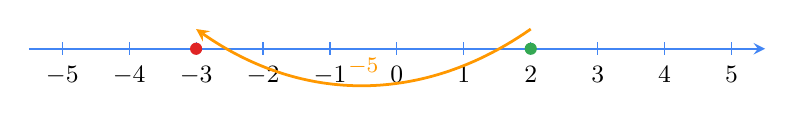
\begin{tikzpicture}[x=0.85cm,>=stealth]
\draw[->,thick,Navy] (-5.5,0)--(5.5,0);
\foreach \i in {-5,...,5}{\draw[Navy] (\i,0.08)--(\i,-0.08); \node[below,font=\small] at (\i,-0.1){$\i$};}
\draw[->,tmOrange,line width=1pt] (2,0.25) to[bend left=35] node[above,font=\footnotesize]{$-5$} (-3,0.25);
\fill[tmGreen] (2,0) circle (2.2pt); \fill[AnsRed] (-3,0) circle (2.2pt);
\end{tikzpicture}\end{center}
\emph{Ví dụ:} $2+(-5)=-3$: từ $2$, đi sang trái $5$ bước, đến $-3$.

\textbf{2. Cộng, trừ số nguyên.}
\begin{itemize}[leftmargin=1.4em,itemsep=1pt,topsep=2pt]
\item Cộng hai số cùng dấu: cộng phần số, giữ dấu chung: $(-11)+(-26)=-37$.
\item Cộng hai số khác dấu: lấy phần số lớn trừ phần số nhỏ, lấy dấu của số có phần số lớn hơn: $11+(-37)=-26$.
\item Trừ là cộng với số đối: $a-b=a+(-b)$. Ví dụ: $-26-11=-26+(-11)=-37$.
\end{itemize}

\textbf{3. Thứ tự thực hiện phép tính.} Ngoặc trước $\to$ luỹ thừa $\to$ nhân, chia (từ trái sang phải)
$\to$ cộng, trừ (từ trái sang phải). Ví dụ: $6+2\cdot 3=6+6=12$ (không phải $8\cdot 3$).

\textbf{4. Tính chất phân phối.} $a(b+c)=ab+ac$ và $a(b-c)=ab-ac$.
\emph{Ví dụ:} $3(T+4)=3T+12$;\quad $20\cdot 9\,000-20\cdot 6\,750=20\cdot(9\,000-6\,750)$.

\textbf{5. Thu gọn biểu thức.} Cộng các số hạng ``cùng loại'': $3x+5x=8x$; \
$(a+1)+(b+1)+(c+1)+(d+1)=(a+b+c+d)+4$.

\textbf{6. Điểm trên mặt phẳng toạ độ.} Điểm $(x;y)$ có hoành độ $x$ và tung độ $y$. Đi sang phải $k$
đơn vị thì $x$ tăng $k$; đi lên $k$ đơn vị thì $y$ tăng $k$ (đi sang trái, đi xuống thì giảm).
\end{knowbox}

\begin{proofbox}
\textbf{Vì sao $a(b+c)=ab+ac$?} Xét một hình chữ nhật có chiều rộng $a$, chiều dài $b+c$. Diện tích của nó là
$a(b+c)$. Nhưng ta cũng có thể cắt nó thành hai hình chữ nhật nhỏ có diện tích $ab$ và $ac$. Cùng một
diện tích nên $a(b+c)=ab+ac$.
\begin{figC}
\fill[tmBlue!18] (0,0) rectangle (3,1.2); \fill[tmGreen!20] (3,0) rectangle (5,1.2);
\draw[Navy,line width=0.9pt] (0,0) rectangle (5,1.2); \draw[Navy,line width=0.9pt] (3,0)--(3,1.2);
\node at (1.5,0.6){$ab$}; \node at (4,0.6){$ac$};
\node[left] at (0,0.6){$a$}; \node[below] at (1.5,0){$b$}; \node[below] at (4,0){$c$};
\end{figC}
\end{proofbox}

\begin{warnbox}
$3(T+4)$ \emph{không bằng} $3T+4$: phải nhân $3$ với \emph{từng} số hạng trong ngoặc, $3(T+4)=3T+3\cdot 4=3T+12$.
Tương tự $-(a-b)=-a+b$ (đổi dấu \emph{mọi} số hạng trong ngoặc).
\end{warnbox}

% ------------------------------------------------------------------------------------------
\needspace{6\baselineskip}\shead{Đẳng thức, phương trình và nguyên tắc cân bằng}
\begin{knowbox}
\textbf{1. Phương trình.} Một đẳng thức chứa ẩn, chẳng hạn $2(x+8)=38$, gọi là \textbf{phương trình}.
Số thay vào ẩn làm cho hai vế bằng nhau gọi là \textbf{nghiệm}. \emph{Giải phương trình} là tìm nghiệm.

\textbf{2. Nguyên tắc cân bằng.} Hãy tưởng tượng phương trình là một chiếc cân đang thăng bằng.
Cân vẫn thăng bằng nếu ta:
\begin{itemize}[leftmargin=1.4em,itemsep=1pt,topsep=2pt]
\item cộng (hoặc trừ) \emph{cùng một số} vào cả hai vế;
\item nhân (hoặc chia) cả hai vế với \emph{cùng một số khác $0$}.
\end{itemize}
Hệ quả quen thuộc là \textbf{quy tắc chuyển vế}: chuyển một số hạng từ vế này sang vế kia thì phải \emph{đổi dấu} số hạng đó.

\begin{center}
\aeaScale{\aeaSq\,\aeaSq\ \ \fbox{\footnotesize 3 kg}}{\fbox{\footnotesize 11 kg}}
\end{center}
\emph{Ví dụ:} hai hộp như nhau cùng quả cân $3$ kg cân bằng với $11$ kg: $2x+3=11$.
Bỏ quả cân $3$ kg ở cả hai đĩa: $2x=11-3=8$. Chia đôi cả hai đĩa: $x=8:2=4$. Mỗi hộp nặng $4$ kg.

\textbf{3. Phép thế trên cân.} Nếu một đĩa cân chứa $A$ cân bằng với $B$ thì ở bất kì chiếc cân nào khác, ta có thể
thay $A$ bằng $B$ mà cân vẫn thăng bằng (giống như thay một biểu thức bằng một biểu thức bằng nó).

\textbf{4. Luôn thử lại.} Sau khi giải, thay nghiệm vào phương trình ban đầu để chắc chắn hai vế bằng nhau.
\end{knowbox}

\begin{proofbox}
\textbf{Vì sao chuyển vế phải đổi dấu?} Từ $2x+3=11$, trừ $3$ ở cả hai vế (cân vẫn thăng bằng):
$2x+3-3=11-3$, tức là $2x=11-3$. Nhìn kết quả, ta thấy số hạng $+3$ ở vế trái như đã ``nhảy'' sang vế phải và trở thành $-3$.
Thật ra không có gì ``nhảy'' cả, ta chỉ trừ cùng một số ở hai vế.
\end{proofbox}

\begin{warnbox}
Quên đổi dấu khi chuyển vế: từ $x+11=-26$ mà viết $x=-26+11$ là \textbf{sai}. Đúng là $x=-26-11=-37$.
\end{warnbox}

\begin{tipbox}
Gặp bài trắc nghiệm có phương trình, ta có thể \emph{thay lần lượt từng phương án} vào phương trình. Cách này
chậm hơn nhưng rất chắc chắn, và cũng là cách thử lại tốt nhất.
\end{tipbox}

% ------------------------------------------------------------------------------------------
\needspace{6\baselineskip}\shead{Giải bài toán bằng cách lập phương trình}
\begin{knowbox}
\textbf{Bốn bước giải bài toán có lời văn.}
\begin{enumerate}[leftmargin=1.6em,itemsep=1pt,topsep=2pt]
\item \textbf{Chọn ẩn}: gọi đại lượng cần tìm (hoặc một đại lượng liên quan) là $x$; ghi rõ đơn vị và điều kiện (ví dụ $x>0$, $x$ là số nguyên).
\item \textbf{Biểu diễn} các đại lượng khác theo $x$.
\item \textbf{Lập phương trình} từ điều kiện của đề bài rồi \textbf{giải}.
\item \textbf{Đối chiếu} điều kiện, \textbf{thử lại} và \textbf{trả lời} đúng câu hỏi.
\end{enumerate}

\textbf{Các dạng hay gặp.}
\begin{itemize}[leftmargin=1.4em,itemsep=2pt,topsep=2pt]
\item \textbf{Số nguyên liên tiếp:} $n,\ n+1,\ n+2$ (hoặc gọn hơn $n-1,\ n,\ n+1$). Số chẵn (lẻ) liên tiếp hơn kém nhau $2$: $n,\ n+2,\ n+4$.
\item \textbf{Tổng từng đôi:} ba vật $a,b,c$ cân từng đôi được $a+b$, $b+c$, $c+a$. Cộng ba kết quả:
$(a+b)+(b+c)+(c+a)=2(a+b+c)$, nên \emph{tổng ba vật bằng nửa tổng các kết quả}. Muốn tìm một vật, lấy tổng ba vật trừ đi tổng hai vật kia.
\item \textbf{Góc trong tam giác:} tổng ba góc của một tam giác bằng $180^\circ$; tam giác cân có hai góc ở đáy bằng nhau.
\item \textbf{Trung bình:} giá trị trung bình $=$ tổng các giá trị $:$ số các giá trị; giá trung bình $=$ tổng số tiền $:$ tổng khối lượng.
\end{itemize}
\end{knowbox}

\textbf{Hai ví dụ nhỏ.}

\emph{a) Tam giác cân có một góc $70^\circ$.} Góc $70^\circ$ có thể là \emph{góc ở đáy} hoặc \emph{góc ở đỉnh}, nên phải xét hai trường hợp:
\begin{itemize}[leftmargin=1.4em,itemsep=1pt,topsep=1pt]
\item Nếu $70^\circ$ là góc ở đáy: hai góc đáy là $70^\circ$ và $70^\circ$, góc ở đỉnh là $180^\circ-70^\circ-70^\circ=40^\circ$.
\item Nếu $70^\circ$ là góc ở đỉnh: hai góc đáy bằng nhau và có tổng $180^\circ-70^\circ=110^\circ$, mỗi góc là $55^\circ$.
\end{itemize}
\begin{figC}
\draw[tmBlue,line width=1pt,fill=tmBlue!8] (0,0)--(2.4,0)--(1.2,3.3)--cycle;
\node[font=\footnotesize] at (0.45,0.25){$70^\circ$}; \node[font=\footnotesize] at (1.95,0.25){$70^\circ$}; \node[font=\footnotesize] at (1.2,2.6){$40^\circ$};
\draw[tmOrange!85!black,line width=1pt,fill=tmOrange!10] (4,0)--(7.4,0)--(5.7,2.43)--cycle;
\node[font=\footnotesize] at (4.55,0.22){$55^\circ$}; \node[font=\footnotesize] at (6.85,0.22){$55^\circ$}; \node[font=\footnotesize] at (5.7,1.85){$70^\circ$};
\end{figC}

\emph{b) Giá trung bình.} Mua $300$ g kẹo loại I hết $15\,000$ đồng và $200$ g kẹo loại II hết $20\,000$ đồng. Giá trung bình của
$100$ g kẹo là $(15\,000+20\,000):(300+200)\cdot 100=35\,000:500\cdot 100=7\,000$ đồng.
\emph{Không} được lấy trung bình của hai giá $5\,000$ và $10\,000$ đồng cho mỗi $100$ g (sẽ ra $7\,500$ đồng, sai), vì hai loại kẹo được mua với khối lượng khác nhau.

\begin{proofbox}
\textbf{Ba số nguyên liên tiếp: số ở giữa bằng tổng chia $3$.} Gọi ba số là $n-1$, $n$, $n+1$. Tổng của chúng là
$(n-1)+n+(n+1)=3n$ (vì $-1$ và $+1$ triệt tiêu). Vậy số ở giữa $n=\text{tổng}:3$. Chẳng hạn tổng là $153$ thì số giữa là $51$ và ba số là $50,51,52$.
\end{proofbox}

\begin{tipbox}
Đặt ẩn là \emph{số ở giữa} thường làm phương trình gọn nhất. Với các bài ``tổng từng đôi'', đừng vội đặt ba ẩn và giải hệ:
hãy \emph{cộng tất cả lại} trước.
\end{tipbox}

\begin{warnbox}
Giải xong phương trình chưa phải là xong bài! Phải đọc lại câu hỏi: đề hỏi số \emph{lớn nhất}, vật \emph{nhẹ nhất}, hay \emph{tổng}...?
Rất nhiều bạn tìm đúng $x$ nhưng chọn sai đáp án vì trả lời nhầm câu hỏi.
\end{warnbox}

\begin{parentbox}
Khi con bí, hãy hỏi: ``Cái gì mình chưa biết? Gọi nó là $x$ nhé. Bây giờ, đề bài nói gì về $x$?''
Hãy để con nói thành lời trước, rồi mới viết thành phương trình.
\end{parentbox}

% ------------------------------------------------------------------------------------------
\needspace{6\baselineskip}\shead{Quy luật, bảng giá trị và dãy số cách đều}
\begin{knowbox}
\textbf{1. Dãy số cách đều.} Một dãy số mà hai số liền nhau luôn hơn kém nhau cùng một số $d$ (gọi là
\textbf{khoảng cách} hay \textbf{công sai}) được gọi là dãy cách đều. Nếu số hạng đầu là $a$ thì
\[\text{số hạng thứ } n \;=\; a+(n-1)\cdot d .\]
\emph{Ví dụ:} dãy $7,10,13,16,\dots$ có $a=7$, $d=3$; số hạng thứ $n$ là $7+3(n-1)=3n+4$.

\textbf{2. Từ bảng giá trị đến biểu thức.} Khi $n$ tăng $1$ mà giá trị luôn tăng $d$, biểu thức có dạng
$d\cdot n+\text{(một số)}$. Tìm ``một số'' bằng cách thay $n=1$.
\begin{center}
\begin{tabular}{|c|c|c|c|c|c|}
\hline
\rowcolor{tmBlue!10} $n$ & $1$ & $2$ & $3$ & $4$ & $5$\\ \hline
giá trị & $4$ & $7$ & $10$ & $13$ & $16$\\ \hline
\end{tabular}
\end{center}
Mỗi lần $n$ tăng $1$, giá trị tăng $3$ nên biểu thức có dạng $3n+b$. Thay $n=1$: $3+b=4$, suy ra $b=1$. Vậy giá trị $=3n+1$.

\textbf{3. Một số có nằm trong dãy không?} Số $N$ thuộc dãy $a,\ a+d,\ a+2d,\dots$ khi và chỉ khi
$N-a$ chia hết cho $d$ (và $N\ge a$). Với dãy đếm lùi $a,\ a-d,\ a-2d,\dots$ thì xét $a-N$.

\textbf{4. Số chung của hai dãy; hiện tượng lặp lại.} Nếu hai dãy cách đều có khoảng cách $d_1$, $d_2$ có một số chung thì
các số chung cách nhau đúng $\text{BCNN}(d_1,d_2)$. Tương tự, những sự việc lặp lại sau $p$ phút và sau $q$ phút sẽ
cùng xảy ra lại sau mỗi $\text{BCNN}(p,q)$ phút.
\end{knowbox}

\begin{tipbox}
\emph{Ví dụ về sự lặp lại.} Xe buýt thứ nhất cứ $12$ phút lại về bến, xe thứ hai cứ $20$ phút lại về bến. Lúc $7\,h$ cả hai cùng ở bến.
Thời điểm xe thứ nhất về bến: sau $12, 24, 36, 48, \mathbf{60},\dots$ phút; xe thứ hai: sau $20, 40, \mathbf{60},\dots$ phút.
Hai xe lại gặp nhau ở bến sau mỗi $\text{BCNN}(12,20)=60$ phút, tức lúc $8\,h$, $9\,h$, \dots

Tương tự, hai dãy $7,10,13,\dots$ (cách $3$) và $2011,2006,2001,\dots$ (cách $5$) nếu có số chung thì các số chung cách nhau $\text{BCNN}(3,5)=15$.
\end{tipbox}

\begin{proofbox}
\textbf{Vì sao số hạng thứ $n$ là $a+(n-1)d$?} Đi từ số hạng thứ $1$ đến số hạng thứ $n$, ta bước qua $n-1$ ``khoảng'',
mỗi khoảng cộng thêm $d$. Giống như đi từ cột điện thứ $1$ đến cột thứ $5$ chỉ qua $4$ khoảng.
\begin{figC}
\foreach \i/\v in {0/a,1/a+d,2/a+2d,3/a+3d}{\fill[tmBlue] (2.2*\i,0) circle (2.5pt); \node[below,font=\footnotesize] at (2.2*\i,-0.1){$\v$};}
\foreach \i in {0,1,2}{\draw[->,tmOrange,line width=0.9pt] (2.2*\i+0.15,0.15) to[bend left=30] node[above,font=\footnotesize]{$+d$} (2.2*\i+2.05,0.15);}
\node[font=\footnotesize,text=Slate] at (0,0.7){thứ 1}; \node[font=\footnotesize,text=Slate] at (6.6,0.7){thứ 4};
\end{figC}
Từ số thứ $1$ đến số thứ $4$ có $3$ bước $+d$, nên số thứ $4$ là $a+3d$.
\end{proofbox}

\begin{warnbox}
Kiểm tra một công thức chỉ với \emph{một} cột của bảng là chưa đủ. Chẳng hạn bảng $1,3,5,7,9$: cả $3n-2$ lẫn $2n-1$ đều
cho giá trị $1$ khi $n=1$, nhưng với $n=2$ thì $3n-2=4\neq 3$. Hãy thử với \emph{ít nhất hai, ba cột}.
\end{warnbox}

% ------------------------------------------------------------------------------------------
\needspace{6\baselineskip}\shead{Tỉ lệ, đơn vị đo và chuyển động đều}
\begin{knowbox}
\textbf{1. Đại lượng tỉ lệ thuận.} Nếu một thìa thức ăn đủ cho $8$ con cá thì $2$ thìa đủ cho $16$ con, $4$ thìa đủ cho $32$ con:
gấp số thìa lên bao nhiêu lần thì số cá cũng gấp lên bấy nhiêu lần. Ta nói $y$ \textbf{tỉ lệ thuận} với $x$ theo hệ số $k$ nếu $y=k\cdot x$.
Cách giải quen thuộc: \textbf{rút về đơn vị} (tính cho $1$ phần trước, rồi nhân lên).

\textbf{2. Chuyển động đều.} Với $s$ là quãng đường, $v$ là vận tốc, $t$ là thời gian:
\[ s=v\cdot t,\qquad t=\frac{s}{v},\qquad v=\frac{s}{t}.\]
Nhớ dùng đơn vị phù hợp: $v$ tính bằng km/h thì $s$ tính bằng km và $t$ tính bằng giờ.

Hai người chạy \emph{cùng một khoảng thời gian}: ai nhanh gấp $k$ lần thì đi được quãng đường gấp $k$ lần.

\emph{Chạy ngược chiều trên đường tròn:} từ lần gặp nhau này đến lần gặp nhau sau, \emph{tổng} quãng đường hai người chạy được đúng bằng một vòng.
Nếu người thứ nhất nhanh gấp $k$ lần người thứ hai thì trong mỗi lượt đó, người thứ nhất chạy $\dfrac{k}{k+1}$ vòng, người thứ hai chạy $\dfrac{1}{k+1}$ vòng.

\textbf{3. Đổi đơn vị thời gian.}
$1$ phút $=60$ giây;\ \ $1$ giờ $=60$ phút $=60\times 60=3\,600$ giây;\ \ $1$ ngày $=24$ giờ;\ \ $1$ tuần $=7$ ngày.
Do đó $1$ tuần $=7\times 24$ giờ $=7\times 24\times 60$ phút $=7\times 24\times 60\times 60$ giây.

\textbf{4. Tiền.} Số tờ tiền $=$ tổng số tiền $:$ mệnh giá một tờ. \ Tiền chênh lệch sau $n$ lần
$=n\times(\text{giá lớn}-\text{giá nhỏ})$.
\end{knowbox}

\begin{tipbox}
Đọc một tích như $60\times 60\times 24\times 7$ như một \emph{chuỗi đổi đơn vị}, đọc từ phải sang trái:
$7$ (ngày trong một tuần) $\times 24$ (giờ trong một ngày) $\times 60$ (phút trong một giờ) $\times 60$ (giây trong một phút).
Kết quả là số giây trong một tuần.
\end{tipbox}

\begin{proofbox}
\textbf{Vì sao tính chênh lệch ``mỗi lần'' rồi nhân lên cũng được?} Theo tính chất phân phối:
$20\times 9\,000-20\times 6\,750=20\times(9\,000-6\,750)=20\times 2\,250$. Hai cách tính luôn cho cùng một kết quả,
nhưng cách thứ hai nhẩm nhanh hơn nhiều.
\end{proofbox}

\begin{warnbox}
Trong bài chuyển động, đọc kĩ ``đã đi được bao nhiêu'' và ``còn lại bao nhiêu''. Đi được một nửa quãng đường $510$ km
thì quãng đường còn lại là $510:2=255$ km, không phải $510$ km.
\end{warnbox}

% ------------------------------------------------------------------------------------------
\needspace{6\baselineskip}\shead{Phân số bằng nhau và phân số của một số}
\begin{knowbox}
\textbf{1. Tính chất cơ bản.} Nhân (hoặc chia) cả tử và mẫu của một phân số với cùng một số khác $0$,
ta được một phân số bằng nó: $\dfrac{3}{7}=\dfrac{3\cdot 9}{7\cdot 9}=\dfrac{27}{63}$.

\textbf{2. Nhận biết hai phân số bằng nhau.} Với $b\neq 0$, $d\neq 0$:\quad
$\dfrac{a}{b}=\dfrac{c}{d}$ khi và chỉ khi $a\cdot d=b\cdot c$ (``nhân chéo'').

\textbf{3. Hai phân số cùng tử.} Nếu $\dfrac{1}{p}=\dfrac{1}{q}$ (hay $\dfrac{m}{p}=\dfrac{m}{q}$ với $m\neq 0$) thì $p=q$.
Hai phân số có tử bằng nhau và bằng nhau thì mẫu cũng bằng nhau.

\textbf{4. Phân số của một số.} Muốn tìm $\dfrac{m}{n}$ của số $A$, ta tính $A\cdot\dfrac{m}{n}=A:n\cdot m$.
\emph{Ví dụ:} $\dfrac{3}{7}$ của $168$ km là $168:7\cdot 3=24\cdot 3=72$ km. Phần còn lại ứng với $1-\dfrac{3}{7}=\dfrac{4}{7}$.
\end{knowbox}

\begin{proofbox}
\textbf{Vì sao $\dfrac{1}{p}=\dfrac{1}{q}$ kéo theo $p=q$?} Nhân chéo: $1\cdot q=p\cdot 1$, tức là $q=p$.
Nói cách khác: chia một chiếc bánh thành $p$ phần và thành $q$ phần mà mỗi phần to bằng nhau thì số phần phải như nhau.
\end{proofbox}

% ------------------------------------------------------------------------------------------
\needspace{6\baselineskip}\shead{So sánh và suy luận về thứ tự}
\begin{knowbox}
\textbf{1. Tính chất bắc cầu.} Nếu $a<b$ và $b<c$ thì $a<c$. Nhờ đó ta có thể xếp nhiều số thành một hàng: $a<b<c<d$.

\textbf{2. Kĩ thuật ``đặt bằng $k$''.} Khi nhiều biểu thức bằng nhau, ví dụ $a-2=b+2=c+1=d-3$, hãy gọi giá trị chung là $k$:
\[a=k+2,\qquad b=k-2,\qquad c=k-1,\qquad d=k+3.\]
Bây giờ mọi số được so sánh với cùng một mốc $k$; xếp các ``phần thêm'' $-2<-1<+2<+3$ ta được $b<c<a<d$.
\begin{center}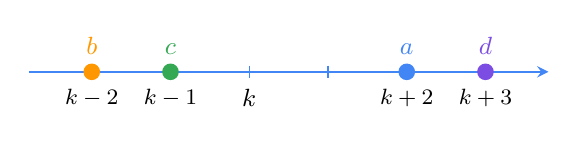
\begin{tikzpicture}[x=1cm,>=stealth]
\draw[->,thick,Navy] (-2.8,0)--(3.8,0);
\foreach \i in {-2,...,3}{\draw[Navy] (\i,0.08)--(\i,-0.08);}
\node[below,font=\small] at (0,-0.1){$k$};
\foreach \i/\l/\c in {-2/b/tmOrange,-1/c/tmGreen,2/a/tmBlue,3/d/tmPurple}{\fill[\c] (\i,0) circle (3pt); \node[above,font=\small\bfseries,text=\c] at (\i,0.1){$\l$};}
\node[below,font=\footnotesize] at (-2,-0.1){$k-2$}; \node[below,font=\footnotesize] at (-1,-0.1){$k-1$};
\node[below,font=\footnotesize] at (2,-0.1){$k+2$}; \node[below,font=\footnotesize] at (3,-0.1){$k+3$};
\end{tikzpicture}\end{center}

\textbf{3. Suy luận logic về thứ tự.} Với các câu như ``An có nhiều mèo hơn Bình'', hãy dịch thành kí hiệu ($A>B$),
viết tất cả các điều kiện ra rồi nối chúng bằng tính chất bắc cầu. Một khẳng định ``\emph{chắc chắn đúng}'' phải đúng trong
\emph{mọi} trường hợp thoả mãn đề bài; chỉ cần một ví dụ trái ngược là đủ để bác bỏ nó.
\end{knowbox}

\begin{tipbox}
\emph{Ví dụ suy luận.} An cao hơn Bình; Chi thấp hơn Bình; Dũng cao hơn Chi. Ai thấp nhất?
Viết kí hiệu: $A>B$, \ $B>C$, \ $D>C$. Từ $A>B>C$ và $D>C$ ta thấy cả $A$, $B$, $D$ đều cao hơn $C$: \textbf{Chi thấp nhất}.
Nhưng ta \emph{không} biết Dũng cao hơn hay thấp hơn An (chẳng hạn An $1{,}6$ m, Bình $1{,}5$ m, Chi $1{,}2$ m thì Dũng cao $1{,}7$ m hay $1{,}3$ m đều thoả mãn mọi điều kiện), nên câu ``Dũng cao nhất'' \emph{không chắc chắn} đúng.
\end{tipbox}

\begin{warnbox}
Nhìn thấy $a-2$ và $b+2$ bằng nhau, nhiều bạn vội kết luận ``$a$ bé hơn vì bị trừ''. Ngược lại mới đúng: $a$ phải \emph{bớt đi} $2$
mới bằng $b$ \emph{thêm} $2$, nên $a$ lớn hơn $b$ đúng $4$ đơn vị.
\end{warnbox}

\begin{parentbox}
Hãy dùng đồ vật thật: ``Túi của con bớt $2$ viên bi thì bằng túi của mẹ thêm $2$ viên. Túi nào nhiều hơn?''
Cho con dùng bi để kiểm tra. Hình ảnh cụ thể giúp con không bị đánh lừa bởi dấu cộng, dấu trừ.
\end{parentbox}

% ==========================================================================================
\needspace{6\baselineskip}\shead{Ví dụ mẫu}

\begin{exbox}{Ví dụ 1 \ (Dịch lời văn và tính giá trị biểu thức)}
\textbf{a)} Tính giá trị của biểu thức $A=2x^2-3x+1$ tại $x=-2$.

\textbf{b)} Bạn Hoa đang có $50\,000$ đồng trong ống heo. Mỗi tuần Hoa bỏ thêm vào $20\,000$ đồng.
Viết biểu thức biểu thị số tiền trong ống heo sau $t$ tuần, rồi tính số tiền đó sau $6$ tuần.
\guide
\step{1}{Câu a: thay $x=-2$, nhớ đặt trong ngoặc}
\[A=2\cdot(-2)^2-3\cdot(-2)+1.\]
\step{2}{Tính theo thứ tự: luỹ thừa $\to$ nhân $\to$ cộng, trừ}
$(-2)^2=(-2)\cdot(-2)=4$, nên $2\cdot 4=8$. \ $3\cdot(-2)=-6$, nên $-3\cdot(-2)=+6$. Vậy $A=8+6+1=15$.
\step{3}{Câu b: tìm quy luật bằng một bảng nhỏ}
\begin{center}
\begin{tabular}{|c|c|c|c|c|}
\hline
\rowcolor{tmBlue!10} Số tuần & $0$ & $1$ & $2$ & $t$\\ \hline
Số tiền (đồng) & $50\,000$ & $50\,000+20\,000$ & $50\,000+2\cdot 20\,000$ & $50\,000+20\,000t$\\ \hline
\end{tabular}
\end{center}
Số tiền có sẵn không đổi; phần bỏ thêm bằng $20\,000$ nhân với số tuần. Biểu thức: $50\,000+20\,000t$ (đồng).
\step{4}{Thay $t=6$}
$50\,000+20\,000\cdot 6=50\,000+120\,000=170\,000$ (đồng).
\begin{warnbox}Không viết $(50\,000+20\,000)\cdot t$: số tiền ban đầu chỉ có \emph{một lần}, không được nhân với số tuần.\end{warnbox}
\ans{a) $A=15$;\ \ b) $50\,000+20\,000t$ đồng; sau $6$ tuần có $170\,000$ đồng.}
\end{exbox}

\begin{exbox}{Ví dụ 2 \ (Giải phương trình bằng nguyên tắc cân bằng)}
Giải các phương trình:\quad \textbf{a)} $5x-7=2x+11$;\qquad \textbf{b)} $\dfrac{x}{12}=\dfrac{5}{4}$.
\guide
\step{1}{Câu a: gom các số hạng chứa $x$ về vế trái}
Trừ $2x$ ở cả hai vế: $5x-2x-7=11$, tức là $3x-7=11$.
\step{2}{Gom các số về vế phải}
Cộng $7$ vào cả hai vế: $3x=11+7=18$.
\step{3}{Chia cả hai vế cho $3$}
$x=18:3=6$.
\verify{Vế trái: $5\cdot 6-7=30-7=23$. Vế phải: $2\cdot 6+11=12+11=23$. Hai vế bằng nhau.}
\step{4}{Câu b: quy về cùng mẫu (hoặc nhân chéo)}
Ta có $\dfrac{5}{4}=\dfrac{5\cdot 3}{4\cdot 3}=\dfrac{15}{12}$. Hai phân số $\dfrac{x}{12}$ và $\dfrac{15}{12}$ có cùng mẫu
và bằng nhau nên $x=15$. (Nhân chéo cũng được: $4x=12\cdot 5=60$, $x=60:4=15$.)
\begin{recallbox}$\dfrac{a}{b}=\dfrac{c}{d}$ khi và chỉ khi $ad=bc$ ($b,d\neq 0$).\end{recallbox}
\ans{a) $x=6$;\ \ b) $x=15$.}
\end{exbox}

\begin{exbox}{Ví dụ 3 \ (Số chẵn liên tiếp)}
Tổng của bốn số chẵn liên tiếp bằng $116$. Tìm số lớn nhất trong bốn số đó.
\guide
\step{1}{Chọn ẩn}
Gọi số chẵn bé nhất là $n$ ($n$ là số chẵn). Hai số chẵn liên tiếp hơn kém nhau $2$, nên bốn số là
$n,\ n+2,\ n+4,\ n+6$.
\step{2}{Lập phương trình}
$n+(n+2)+(n+4)+(n+6)=116$, tức là $4n+12=116$.
\step{3}{Giải}
$4n=116-12=104$, \ $n=104:4=26$. Bốn số là $26,\ 28,\ 30,\ 32$.
\verify{$26+28+30+32=116$. Đúng.}
\step{4}{Trả lời đúng câu hỏi}
Đề hỏi số \emph{lớn nhất}: đó là $32$.
\begin{tipbox}Cách nhẩm: bốn số cách đều nên trung bình của chúng là $116:4=29$, nằm chính giữa hai số giữa $28$ và $30$. Từ đó suy ra ngay bốn số.\end{tipbox}
\ans{$32$}
\end{exbox}

\begin{exbox}{Ví dụ 4 \ (Cân từng đôi)}
Ba bạn Mai, Lan, Hoa lần lượt đứng lên cân từng đôi một. Mai và Lan nặng $72$ kg; Mai và Hoa nặng $78$ kg;
Lan và Hoa nặng $80$ kg. Mỗi bạn nặng bao nhiêu ki-lô-gam?
\guide
\step{1}{Cộng cả ba lần cân}
Trong ba lần cân, mỗi bạn được cân đúng \emph{hai} lần:
$(M+L)+(M+H)+(L+H)=72+78+80=230$, tức là $2(M+L+H)=230$.
\step{2}{Tổng khối lượng ba bạn}
$M+L+H=230:2=115$ (kg).
\step{3}{Tìm từng bạn: lấy tổng trừ đi cặp không chứa bạn đó}
Hoa $=115-(M+L)=115-72=43$ kg;\quad Lan $=115-(M+H)=115-78=37$ kg;\quad Mai $=115-(L+H)=115-80=35$ kg.
\begin{figC}
\foreach \y/\a/\b/\ca/\cb/\s in {0/Mai/Lan/tmBlue/tmOrange/72,-0.8/Mai/Hoa/tmBlue/tmGreen/78,-1.6/Lan/Hoa/tmOrange/tmGreen/80}{
  \node[draw=\ca!80!black,fill=\ca!15,rounded corners=2pt,minimum width=1.4cm] at (0,\y){\a};
  \node at (0.95,\y){$+$};
  \node[draw=\cb!80!black,fill=\cb!15,rounded corners=2pt,minimum width=1.4cm] at (1.9,\y){\b};
  \node[anchor=west] at (2.7,\y){$=\s$ kg};}
\end{figC}
\verify{$35+37=72$, \ $35+43=78$, \ $37+43=80$. Cả ba lần cân đều khớp.}
\ans{Mai $35$ kg, Lan $37$ kg, Hoa $43$ kg.}
\end{exbox}

\begin{exbox}{Ví dụ 5 \ (Dãy cách đều)}
Cho dãy số $4,\ 7,\ 10,\ 13,\ \dots$ (mỗi số hơn số liền trước $3$ đơn vị).
\textbf{a)} Viết biểu thức của số hạng thứ $n$.\quad \textbf{b)} Tính số hạng thứ $50$.\quad
\textbf{c)} Số $2026$ có thuộc dãy không? Nếu có, đó là số hạng thứ mấy?
\guide
\step{1}{Số hạng thứ $n$}
Số hạng đầu $a=4$, khoảng cách $d=3$: số hạng thứ $n$ là $4+3(n-1)=4+3n-3=3n+1$.
\begin{recallbox}Số hạng thứ $n$ của dãy cách đều $=a+(n-1)d$.\end{recallbox}
\step{2}{Số hạng thứ $50$}
$3\cdot 50+1=151$.
\step{3}{Kiểm tra số $2026$}
Ta cần một số tự nhiên $n$ sao cho $3n+1=2026$, tức là $3n=2025$. Vì $2025:3=675$ (chia hết), nên $n=675$.
\verify{$3\cdot 675+1=2025+1=2026$. Đúng.}
\begin{warnbox}Đừng quên kiểm tra phép chia có chia hết hay không. Chẳng hạn $2027$ \emph{không} thuộc dãy vì $2026$ không chia hết cho $3$.\end{warnbox}
\ans{a) $3n+1$;\ \ b) $151$;\ \ c) có, là số hạng thứ $675$.}
\end{exbox}

\begin{exbox}{Ví dụ 6 \ (Chuyển động, phân số và đổi đơn vị)}
Một đoàn tàu chạy đều với vận tốc $72$ km/h trên quãng đường dài $360$ km. Tàu đã đi được $\dfrac{2}{3}$ quãng đường.
Hỏi tàu cần chạy thêm bao lâu nữa (tính ra giờ và phút) thì đến nơi?
\guide
\step{1}{Quãng đường đã đi}
$\dfrac{2}{3}$ của $360$ km là $360:3\cdot 2=120\cdot 2=240$ km.
\step{2}{Quãng đường còn lại}
$360-240=120$ km. (Hoặc: phần còn lại là $1-\dfrac{2}{3}=\dfrac{1}{3}$ quãng đường, $360:3=120$ km.)
\begin{barfigC}
\blk{0}{5}{0}{0.55}{tmBlue}{đã đi 240 km}
\blk{5}{7.5}{0}{0.55}{tmOrange}{còn 120 km}
\brcup{0}{7.5}{0.55}{360 km}
\end{barfigC}
\step{3}{Thời gian còn lại}
\begin{recallbox}$t=\dfrac{s}{v}$ (thời gian $=$ quãng đường $:$ vận tốc).\end{recallbox}
$t=120:72=\dfrac{120}{72}=\dfrac{5}{3}$ giờ $=1\dfrac{2}{3}$ giờ.
\step{4}{Đổi ra giờ và phút}
$\dfrac{2}{3}$ giờ $=\dfrac{2}{3}\cdot 60=40$ phút. Vậy $t=1$ giờ $40$ phút.
\verify{Trong $1$ giờ $40$ phút $=\dfrac{5}{3}$ giờ, tàu đi được $72\cdot\dfrac{5}{3}=24\cdot 5=120$ km. Đúng bằng quãng đường còn lại.}
\ans{$1$ giờ $40$ phút.}
\end{exbox}

\begin{exbox}{Ví dụ 7 \ (Bài toán chiếc cân)}
Cả hai chiếc cân dưới đây đều thăng bằng. Các hình giống nhau thì nặng bằng nhau.
\begin{center}
\aeaScale{\aeaSq}{\aeaTri\,\aeaCir}\hspace{1.2cm}\aeaScale{\aeaSq\,\aeaCir}{\aeaTri\,\aeaTri\,\aeaTri}
\end{center}
Hỏi hai hình vuông \aeaSq\,\aeaSq\ cân bằng với bao nhiêu hình tròn \aeaCir?
\guide
\step{1}{Viết mỗi chiếc cân thành một đẳng thức}
Kí hiệu $V$, $T$, $O$ là khối lượng hình vuông, tam giác, hình tròn. Cân 1: $V=T+O$. \ Cân 2: $V+O=3T$.
\step{2}{Thế cân 1 vào cân 2}
Ở cân 2, thay hình vuông bằng ``một tam giác và một tròn'' (cân 1 cho phép):
$T+O+O=3T$.
\step{3}{Bỏ bớt những thứ giống nhau ở hai đĩa}
Bỏ một tam giác ở mỗi đĩa: $O+O=T+T$, tức $2O=2T$, nên $O=T$: một hình tròn nặng bằng một tam giác.
\step{4}{Trả lời}
$V=T+O=O+O=2O$, nên $2V=4O$: hai hình vuông cân bằng với $4$ hình tròn.
\verify{Chọn thử $O=T=1$, $V=2$: cân 1: $2=1+1$; cân 2: $2+1=3$. Đúng cả hai.}
\ans{$4$ hình tròn.}
\end{exbox}

\begin{exbox}{Ví dụ 8 \ (Sắp thứ tự nhờ kĩ thuật ``đặt bằng $k$'')}
Các số nguyên dương $a$, $b$, $c$ (đều lớn hơn $5$) thoả mãn\quad
$\dfrac{2}{a+3}=\dfrac{2}{b-1}=\dfrac{2}{c+5}$. Hãy sắp xếp $a$, $b$, $c$ theo thứ tự tăng dần.
\guide
\step{1}{Phân số cùng tử bằng nhau thì mẫu bằng nhau}
Ba phân số có cùng tử là $2$ và bằng nhau, nên các mẫu bằng nhau: $a+3=b-1=c+5$.
\begin{recallbox}Nếu $\dfrac{m}{p}=\dfrac{m}{q}$ với $m\neq 0$ thì $p=q$.\end{recallbox}
\step{2}{Đặt giá trị chung là $k$}
$a+3=k\Rightarrow a=k-3$;\quad $b-1=k\Rightarrow b=k+1$;\quad $c+5=k\Rightarrow c=k-5$.
\step{3}{So sánh với mốc $k$}
$k-5<k-3<k+1$, nên $c<a<b$.
\verify{Chọn $k=12$: $a=9$, $b=13$, $c=7$. Khi đó $\dfrac{2}{12}=\dfrac{2}{12}=\dfrac{2}{12}$ và quả thật $7<9<13$.}
\ans{$c<a<b$.}
\end{exbox}

% ==========================================================================================
\clearpage
\dividerbar{Luyện tập cơ bản}

% ---------------------------------------------------------------- Bài 1
\begin{probbox}{1}{\relax}
Chú Tâm lái ô tô chạy đều với vận tốc $85$ km/h trên một chuyến đi dài $510$ km. Hiện chú đã đi được đúng
một nửa quãng đường. Hỏi chú cần đi thêm bao nhiêu giờ nữa thì hết quãng đường?
\choices{$5$ giờ}{$425$ giờ}{$12$ giờ}{$1{,}5$ giờ}{$3$ giờ}
\end{probbox}
\probsol{
\textbf{Phân tích đề.} \emph{Đã biết:} vận tốc $85$ km/h (không đổi), cả quãng đường $510$ km, đã đi được một nửa.
\emph{Cần tìm:} thời gian để đi nốt phần còn lại.
\step{1}{Tính quãng đường còn lại}
Đã đi được một nửa thì còn lại cũng đúng một nửa: $510:2=255$ (km).
\begin{barfigC}
\blk{0}{3}{0}{0.55}{tmBlue}{đã đi 255 km}
\blk{3}{6}{0}{0.55}{tmOrange}{còn 255 km}
\brcup{0}{6}{0.55}{510 km}
\end{barfigC}
\step{2}{Tính thời gian đi hết quãng đường còn lại}
\begin{recallbox}Quãng đường $=$ vận tốc $\times$ thời gian, nên thời gian $=$ quãng đường $:$ vận tốc ($t=\dfrac{s}{v}$).\end{recallbox}
$t=255:85=3$ (giờ). (Nhẩm: $85\times 3=255$.)
\begin{warnbox}Nếu lấy cả quãng đường $510:85=6$ giờ thì đó là thời gian của \emph{cả} chuyến đi, chưa trả lời đúng câu hỏi. Còn $510-85=425$ là phép tính vô nghĩa (trừ km cho km/h), đó là cái bẫy ở phương án (B).\end{warnbox}
\begin{tipbox}Cách khác: cả chuyến đi mất $510:85=6$ giờ; đã đi một nửa quãng đường (với vận tốc không đổi) tức là đã đi một nửa thời gian, nên còn $6:2=3$ giờ.\end{tipbox}
\verify{Trong $3$ giờ, ô tô đi được $85\times 3=255$ km, đúng bằng quãng đường còn lại.}
Kết quả $3$ giờ ứng với phương án \textbf{(E)}.
\ans{(E) $3$ giờ}
}

% ---------------------------------------------------------------- Bài 2
\begin{probbox}{2}{\relax}
Trong hình vẽ, tam giác có một cạnh dài $14$ cm và hai cạnh bằng nhau, mỗi cạnh dài $12$ cm; hình chữ nhật có chiều rộng
$8$ cm và chiều dài $x$ cm. Biết chu vi tam giác bằng chu vi hình chữ nhật. Tìm $x$.
\begin{figC}
\draw[tmBlue,line width=1.1pt,fill=tmBlue!10] (0,2.6)--(2.8,2.6)--(1.4,1.2)--cycle;
\node[above] at (1.4,2.6){$14$ cm};
\node[right] at (2.15,1.9){$12$ cm};
\draw[tmBlue,line width=0.9pt] ($(0.7,1.9)+(-0.1,-0.1)$)--($(0.7,1.9)+(0.1,0.1)$);
\draw[tmBlue,line width=0.9pt] ($(2.1,1.9)+(-0.1,0.1)$)--($(2.1,1.9)+(0.1,-0.1)$);
\draw[tmOrange!85!black,line width=1.1pt,fill=tmOrange!12] (0.4,0)rectangle(2.4,0.9);
\node[right] at (2.4,0.45){$8$ cm};
\node[below] at (1.4,0){$x$ cm};
\end{figC}
\choices{$8$}{$10$}{$11$}{$14$}{$15$}
\end{probbox}
\probsol{
\textbf{Phân tích đề.} Tam giác có ba cạnh $14$ cm, $12$ cm, $12$ cm (hai vạch nhỏ trên hình cho biết hai cạnh đó bằng nhau).
Hình chữ nhật có hai kích thước $x$ cm và $8$ cm. Hai chu vi bằng nhau. Cần tìm $x$.
\step{1}{Tính chu vi tam giác}
\begin{recallbox}Chu vi tam giác bằng tổng độ dài ba cạnh. Chu vi hình chữ nhật bằng $2\times(\text{dài}+\text{rộng})$.\end{recallbox}
Chu vi tam giác: $14+12+12=38$ (cm).
\begin{warnbox}Hình vẽ chỉ ghi số $12$ một lần, nhưng có \emph{hai} cạnh dài $12$ cm (có vạch đánh dấu bằng nhau). Nếu quên cạnh thứ ba, ta sẽ được $26$ cm và giải sai.\end{warnbox}
\step{2}{Lập phương trình}
Chu vi hình chữ nhật là $2(x+8)$. Cho hai chu vi bằng nhau: $2(x+8)=38$.
\step{3}{Giải phương trình}
Chia cả hai vế cho $2$: $x+8=19$. Trừ $8$ ở cả hai vế: $x=19-8=11$.
\verify{Hình chữ nhật $11$ cm $\times$ $8$ cm có chu vi $11+8+11+8=38$ cm, đúng bằng chu vi tam giác.}
Giá trị $x=11$ ứng với phương án \textbf{(C)}.
\begin{parentbox}Có thể minh hoạ bằng một sợi dây dài $38$ cm: uốn thành tam giác $14$ -- $12$ -- $12$, rồi uốn lại thành hình chữ nhật có cạnh $8$ cm. Con sẽ thấy ``chu vi'' chính là độ dài sợi dây, không đổi khi đổi hình.\end{parentbox}
\ans{(C) $11$}
}

% ---------------------------------------------------------------- Bài 3
\begin{probbox}{3}{\relax}
Cho $x=3$. Đẳng thức nào dưới đây đúng?
\choices{$2x=5$}{$3x-1=8$}{$x+5=3$}{$7-x=2$}{$6+2x=14$}
\end{probbox}
\probsol{
\textbf{Phân tích đề.} Ta thay $x=3$ vào vế trái của từng đẳng thức, tính ra số, rồi so sánh với vế phải. Chỉ có một đẳng thức đúng.
\begin{recallbox}Muốn tính giá trị của biểu thức, ta thay chữ bằng số rồi thực hiện phép tính theo thứ tự: nhân, chia trước; cộng, trừ sau.\end{recallbox}
\step{1}{Kiểm tra lần lượt từng phương án}
\begin{center}
\begin{tabular}{|c|l|c|c|}
\hline
\rowcolor{tmBlue!10} Phương án & Thay $x=3$ vào vế trái & Vế phải & Đúng/Sai\\ \hline
(A) & $2x=2\cdot 3=6$ & $5$ & Sai\\ \hline
(B) & $3x-1=3\cdot 3-1=9-1=8$ & $8$ & \textbf{Đúng}\\ \hline
(C) & $x+5=3+5=8$ & $3$ & Sai\\ \hline
(D) & $7-x=7-3=4$ & $2$ & Sai\\ \hline
(E) & $6+2x=6+2\cdot 3=6+6=12$ & $14$ & Sai\\ \hline
\end{tabular}
\end{center}
\begin{warnbox}Ở (E), nếu tính sai thứ tự là $(6+2)\cdot 3=24$ hoặc đọc $2x$ thành ``$23$'' thì sẽ bị nhầm. Nhân trước, cộng sau: $6+2\cdot 3=12$.\end{warnbox}
\step{2}{Kết luận}
Chỉ có đẳng thức ở (B) đúng: $3\cdot 3-1=8$. Vậy chọn \textbf{(B)}.
\ans{(B) $3x-1=8$}
}

% ---------------------------------------------------------------- Bài 4
\begin{probbox}{4}{\relax}
Tổng của ba số nguyên liên tiếp bằng $153$. Số lớn nhất trong ba số đó là
\choices{$52$}{$50$}{$53$}{$54$}{$51$}
\end{probbox}
\probsol{
\textbf{Phân tích đề.} Ba số nguyên liên tiếp là ba số đứng liền nhau trên trục số, hơn kém nhau $1$ (ví dụ $7,8,9$). Biết tổng là $153$. Cần tìm số \emph{lớn nhất}.
\step{1}{Chọn ẩn: gọi số ở giữa là $n$}
Ba số là $n-1$, \ $n$, \ $n+1$.
\step{2}{Lập phương trình}
$(n-1)+n+(n+1)=153$. Ở vế trái, $-1$ và $+1$ triệt tiêu nhau, còn lại $3n=153$.
\step{3}{Giải}
$n=153:3=51$. Ba số là $50$, $51$, $52$.
\begin{recallbox}Với ba số nguyên liên tiếp, số ở giữa bằng tổng chia cho $3$ (số ở giữa chính là trung bình cộng).\end{recallbox}
\begin{proofbox}Cách khác, gọi số bé nhất là $m$: $m+(m+1)+(m+2)=3m+3=153$, nên $3m=150$, $m=50$. Cùng ra ba số $50,51,52$.\end{proofbox}
\begin{tipbox}Mẹo trắc nghiệm: số lớn nhất phải lớn hơn trung bình $153:3=51$ một chút; thử ngay $50+51+52=153$.\end{tipbox}
\verify{$50+51+52=153$. Đúng.}
\step{4}{Trả lời đúng câu hỏi}
Số lớn nhất là $52$, ứng với phương án \textbf{(A)}.
\begin{warnbox}Phương án (E) $51$ là số \emph{ở giữa}, phương án (B) $50$ là số \emph{bé nhất}. Đọc kĩ câu hỏi để khỏi chọn nhầm.\end{warnbox}
\ans{(A) $52$}
}

% ---------------------------------------------------------------- Bài 5
\begin{probbox}{5}{\relax}
Mỗi thìa thức ăn cho cá đủ cho $8$ con cá vàng ăn. Hỏi $4$ thìa thức ăn như thế đủ cho bao nhiêu con cá vàng?
\choices{$12$}{$16$}{$8$}{$64$}{$32$}
\end{probbox}
\probsol{
\textbf{Phân tích đề.} $1$ thìa $\to$ $8$ con cá. Hỏi $4$ thìa $\to$ ? con cá.
Số thìa gấp lên bao nhiêu lần thì số cá được cho ăn cũng gấp lên bấy nhiêu lần (hai đại lượng tỉ lệ thuận).
\begin{recallbox}Nếu $y$ tỉ lệ thuận với $x$ theo hệ số $k$ thì $y=k\cdot x$. Ở đây $k=8$ (con cá cho mỗi thìa), nên số cá $=8\times$ số thìa.\end{recallbox}
\step{1}{Vẽ sơ đồ}
\begin{barfigC}
\blk{0}{1.5}{0}{0.55}{tmGreen}{8 con}
\blk{1.5}{3}{0}{0.55}{tmGreen}{8 con}
\blk{3}{4.5}{0}{0.55}{tmGreen}{8 con}
\blk{4.5}{6}{0}{0.55}{tmGreen}{8 con}
\brcup{0}{6}{0.55}{4 thìa}
\end{barfigC}
\step{2}{Tính}
$4\times 8=32$ (con cá).
\begin{warnbox}Phương án (A) $12$ là $8+4$ (cộng thay vì nhân), phương án (D) $64$ là $8\times 8$. Mỗi thìa thêm vào cho \emph{thêm $8$ con}, nên phải nhân $8$ với số thìa.\end{warnbox}
\verify{$32:4=8$: mỗi thìa đúng $8$ con.}
Vậy chọn \textbf{(E)}.
\ans{(E) $32$}
}

% ---------------------------------------------------------------- Bài 6
\begin{probbox}{6}{\relax}
Cho $x=4$ và $y=3x$. Giá trị của $y$ là
\choices{$12$}{$24$}{$7$}{$81$}{$4$}
\end{probbox}
\probsol{
\textbf{Phân tích đề.} Biết $x=4$. Biểu thức $y=3x$ nghĩa là ``$y$ bằng $3$ nhân $x$''. Cần tính $y$.
\begin{recallbox}$3x$ là cách viết gọn của $3\cdot x$ (giữa số và chữ ta bỏ dấu nhân).\end{recallbox}
\step{1}{Thay $x=4$}
$y=3\cdot x=3\cdot 4=12$.
\begin{warnbox}Không được đọc $3x$ thành ``$34$'' (ghép chữ số), cũng không phải $3+4=7$ (phương án C) hay $3^4=81$ (phương án D).\end{warnbox}
\begin{tipbox}Có thể đọc $y=3x$ thành lời: ``$y$ gấp ba lần $x$''. Gấp ba lần $4$ là $12$.\end{tipbox}
\verify{$12:3=4=x$. Đúng.}
Vậy chọn \textbf{(A)}.
\ans{(A) $12$}
}

% ---------------------------------------------------------------- Bài 7
\begin{probbox}{7}{\relax}
Mỗi lần đi xe buýt, bạn Lan trả $6\,750$ đồng, còn bạn Minh trả $9\,000$ đồng (hai bạn đi hai tuyến khác nhau).
Nếu mỗi bạn đi xe buýt $20$ lần thì tổng cộng Lan trả ít hơn Minh bao nhiêu tiền?
\choicesII{$75\,000$ đồng}{$30\,000$ đồng}{$45\,000$ đồng}{$135\,000$ đồng}{$180\,000$ đồng}
\end{probbox}
\probsol{
\textbf{Phân tích đề.} Mỗi lần: Lan $6\,750$ đồng, Minh $9\,000$ đồng. Mỗi bạn đi $20$ lần. Hỏi \emph{số tiền chênh lệch} sau $20$ lần.
\step{1}{Cách 1 -- Tính tổng của từng bạn rồi trừ}
Lan trả: $20\times 6\,750=135\,000$ (đồng).\quad Minh trả: $20\times 9\,000=180\,000$ (đồng).\\
Chênh lệch: $180\,000-135\,000=45\,000$ (đồng).
\step{2}{Cách 2 -- Tính chênh lệch mỗi lần rồi nhân lên (nhanh hơn)}
Mỗi lần Lan trả ít hơn Minh: $9\,000-6\,750=2\,250$ (đồng).\\
Sau $20$ lần: $20\times 2\,250=45\,000$ (đồng).
\begin{recallbox}Tính chất phân phối: $20\times 9\,000-20\times 6\,750=20\times(9\,000-6\,750)$. Vì vậy hai cách luôn cho cùng kết quả.\end{recallbox}
\begin{warnbox}Phương án (D) $135\,000$ đồng là \emph{tổng số tiền của Lan}, phương án (E) $180\,000$ đồng là \emph{tổng số tiền của Minh}. Đề hỏi số tiền \emph{ít hơn}, tức là hiệu.\end{warnbox}
\verify{$135\,000+45\,000=180\,000$. Đúng.}
Vậy chọn \textbf{(C)}.
\ans{(C) $45\,000$ đồng}
}

% ---------------------------------------------------------------- Bài 8
\begin{probbox}{8}{\relax}
Biểu thức nào cho đúng các giá trị ở hàng thứ hai của bảng, ứng với mỗi giá trị $n$ ở hàng thứ nhất?
\begin{center}
\begin{tabular}{|c|c|c|c|c|c|}
\hline
\rowcolor{tmBlue!10} $n$ & $1$ & $2$ & $3$ & $4$ & $5$\\ \hline
Giá trị & $1$ & $3$ & $5$ & $7$ & $9$\\ \hline
\end{tabular}
\end{center}
\choices{$3n-2$}{$2(n-1)$}{$n+4$}{$2n$}{$2n-1$}
\end{probbox}
\probsol{
\textbf{Phân tích đề.} Ta cần một biểu thức chứa $n$ mà khi thay $n=1,2,3,4,5$ thì lần lượt được $1,3,5,7,9$.
\step{1}{Tìm quy luật của hàng giá trị}
Mỗi lần $n$ tăng thêm $1$ thì giá trị tăng thêm $2$ ($1\to 3\to 5\to 7\to 9$). Vậy biểu thức có dạng $2n+b$.
\begin{recallbox}Nếu $n$ tăng $1$ mà giá trị luôn tăng $d$ thì biểu thức có dạng $d\cdot n+b$; tìm $b$ bằng cách thay $n=1$.\end{recallbox}
\step{2}{Tìm $b$}
Thay $n=1$: $2\cdot 1+b=1$, suy ra $b=1-2=-1$. Biểu thức là $2n-1$.
\step{3}{Kiểm tra cả bảng và loại các phương án khác}
\begin{center}
\begin{tabular}{|c|c|c|c|c|c|c|}
\hline
\rowcolor{tmBlue!10} $n$ & $1$ & $2$ & $3$ & $4$ & $5$ & Kết luận\\ \hline
(A) $3n-2$ & $1$ & $4$ & & & & sai từ $n=2$\\ \hline
(B) $2(n-1)$ & $0$ & & & & & sai ngay $n=1$\\ \hline
(C) $n+4$ & $5$ & & & & & sai ngay $n=1$\\ \hline
(D) $2n$ & $2$ & & & & & sai ngay $n=1$\\ \hline
(E) $2n-1$ & $1$ & $3$ & $5$ & $7$ & $9$ & \textbf{đúng cả bảng}\\ \hline
\end{tabular}
\end{center}
\begin{warnbox}Phương án (A) $3n-2$ cũng cho giá trị $1$ khi $n=1$. Nếu chỉ thử cột đầu tiên, ta sẽ không biết chọn (A) hay (E). Phải thử thêm cột khác.\end{warnbox}
\verify{$2n-1$ với $n=1,2,3,4,5$: $1,3,5,7,9$. Khớp toàn bộ bảng.}
Vậy chọn \textbf{(E)}.
\ans{(E) $2n-1$}
}

% ---------------------------------------------------------------- Bài 9
\begin{probbox}{9}{\relax}
Cộng hai số với nhau, ta được kết quả là $-26$. Biết một trong hai số là $11$. Số còn lại là
\choices{$-37$}{$37$}{$-15$}{$15$}{$-48$}
\end{probbox}
\probsol{
\textbf{Phân tích đề.} Gọi số chưa biết là $x$. Đề bài cho: $x+11=-26$. Cần tìm $x$.
\step{1}{Lập phương trình}
$x+11=-26$.
\step{2}{Giải bằng nguyên tắc cân bằng}
Trừ $11$ ở cả hai vế: $x=-26-11$.
\begin{recallbox}Trừ một số là cộng với số đối của nó: $-26-11=-26+(-11)$. Cộng hai số âm: cộng phần số, giữ dấu ``$-$'': $-(26+11)=-37$.\end{recallbox}
Vậy $x=-37$.
\begin{center}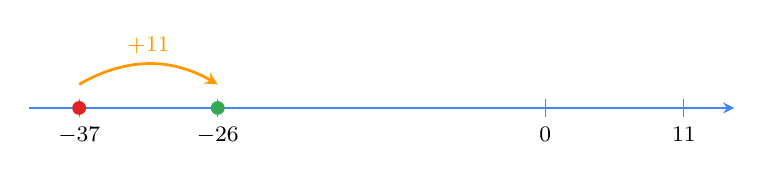
\begin{tikzpicture}[x=0.16cm,>=stealth]
\draw[->,thick,Navy] (-41,0)--(15,0);
\foreach \i in {-37,-26,0,11}{\draw[Navy] (\i,0.12)--(\i,-0.12); \node[below,font=\footnotesize] at (\i,-0.12){$\i$};}
\fill[AnsRed] (-37,0) circle (2.5pt); \fill[tmGreen] (-26,0) circle (2.5pt);
\draw[->,tmOrange,line width=1pt] (-37,0.3) to[bend left=30] node[above,font=\footnotesize]{$+11$} (-26,0.3);
\end{tikzpicture}\end{center}
Trên trục số: từ $-37$ đi sang phải $11$ bước thì đến $-26$.
\begin{warnbox}Quên đổi dấu khi chuyển vế, viết $x=-26+11=-15$, là sai (phương án C). Thử lại: $-15+11=-4\neq -26$.\end{warnbox}
\begin{parentbox}Có thể giải thích bằng chuyện nợ tiền: ``Sau khi được cho $11$ nghìn, bạn vẫn còn nợ $26$ nghìn. Lúc đầu bạn nợ bao nhiêu?'' Lúc đầu nợ nhiều hơn: $26+11=37$ nghìn, tức là $-37$.\end{parentbox}
\verify{$(-37)+11=-26$. Đúng.}
Vậy chọn \textbf{(A)}.
\ans{(A) $-37$}
}

% ---------------------------------------------------------------- Bài 10
\begin{probbox}{10}{\relax}
Bác Hùng có $10\,000\,000$ đồng, toàn bộ là tờ $50\,000$ đồng. Hỏi bác có bao nhiêu tờ tiền?
\choices{$1\,000$}{$200$}{$1\,250$}{$500$}{$2\,000$}
\end{probbox}
\probsol{
\textbf{Phân tích đề.} Tổng số tiền là $10\,000\,000$ đồng (mười triệu đồng). Mỗi tờ có mệnh giá $50\,000$ đồng. Cần tìm số tờ.
\begin{recallbox}Số tờ tiền $=$ tổng số tiền $:$ mệnh giá một tờ.\end{recallbox}
\step{1}{Lập phép chia}
Số tờ $=10\,000\,000:50\,000$.
\step{2}{Tính gọn bằng cách bỏ bớt chữ số $0$}
Bỏ bốn chữ số $0$ ở cả số bị chia và số chia (tức là chia cả hai cho $10\,000$, thương không đổi): $10\,000\,000:50\,000=1\,000:5=200$.
\step{3}{Một cách nghĩ khác}
$2$ tờ $50\,000$ đồng là $100\,000$ đồng. Mười triệu đồng gồm $100$ lần $100\,000$ đồng, nên có $100\times 2=200$ tờ.
\verify{$200\times 50\,000=10\,000\,000$ đồng. Đúng.}
\begin{warnbox}Đếm sai số chữ số $0$ là lỗi rất hay gặp. Nên viết số có dấu cách giữa các nhóm ba chữ số ($10\,000\,000$) để đếm cho chính xác.\end{warnbox}
Vậy chọn \textbf{(B)}.
\begin{parentbox}Nếu nhà có tiền thật, có thể cho con đếm $10$ tờ $50\,000$ đồng ($500\,000$ đồng), rồi hỏi: cần bao nhiêu xấp như vậy để có $10$ triệu? ($20$ xấp, tức $200$ tờ.)\end{parentbox}
\ans{(B) $200$}
}

% ---------------------------------------------------------------- Bài 11
\begin{probbox}{11}{\relax}
Tích $60\times 60\times 24\times 7$ bằng
\choicesL{số phút trong bảy tuần}{số giờ trong sáu mươi ngày}{số giây trong bảy giờ}{số giây trong một tuần}{số phút trong hai mươi bốn tuần}
\end{probbox}
\probsol{
\textbf{Phân tích đề.} Không cần tính tích ra số. Hãy đọc mỗi thừa số như một bước đổi đơn vị thời gian.
\begin{recallbox}$1$ tuần $=7$ ngày;\ \ $1$ ngày $=24$ giờ;\ \ $1$ giờ $=60$ phút;\ \ $1$ phút $=60$ giây.\end{recallbox}
\step{1}{Đọc tích từ phải sang trái}
\begin{itemize}[leftmargin=1.4em,itemsep=1pt,topsep=1pt]
\item $7$ là số ngày trong \textbf{một tuần};
\item $24\times 7$ là số giờ trong một tuần;
\item $60\times 24\times 7$ là số phút trong một tuần;
\item $60\times 60\times 24\times 7$ là số \textbf{giây} trong một tuần.
\end{itemize}
\step{2}{Kiểm tra các phương án còn lại bằng cách viết tích của chúng}
\begin{center}
\begin{tabular}{|c|l|r|}
\hline
\rowcolor{tmBlue!10} Phương án & Biểu thức & Giá trị\\ \hline
(A) phút trong $7$ tuần & $60\times 24\times 7\times 7$ & $70\,560$\\ \hline
(B) giờ trong $60$ ngày & $24\times 60$ & $1\,440$\\ \hline
(C) giây trong $7$ giờ & $60\times 60\times 7$ & $25\,200$\\ \hline
(D) giây trong $1$ tuần & $60\times 60\times 24\times 7$ & $604\,800$\\ \hline
(E) phút trong $24$ tuần & $60\times 24\times 7\times 24$ & $241\,920$\\ \hline
\end{tabular}
\end{center}
Chỉ phương án (D) có đúng tích $60\times 60\times 24\times 7=604\,800$.
\begin{warnbox}Thấy các số $60$, $24$, $7$ xuất hiện trong câu chữ, nhiều bạn chọn vội (A) hoặc (E). Phải ghép đúng \emph{từng} bước đổi đơn vị: (A) thiếu một thừa số $60$ và thừa một thừa số $7$.\end{warnbox}
Vậy chọn \textbf{(D)}.
\ans{(D) số giây trong một tuần}
}

% ---------------------------------------------------------------- Bài 12
\begin{probbox}{12}{\stars{1}}
Bốn số $a$, $b$, $c$, $d$ đều là số nguyên dương lớn hơn $3$ và thoả mãn
\[\frac{1}{a-2}=\frac{1}{b+2}=\frac{1}{c+1}=\frac{1}{d-3}.\]
Cách sắp xếp nào dưới đây là đúng?
\choicesII{$a<b<c<d$}{$c<b<a<d$}{$b<a<c<d$}{$d<a<c<b$}{$b<c<a<d$}
\end{probbox}
\probsol{
\textbf{Phân tích đề.} Bốn phân số có cùng tử số $1$ và bằng nhau. Cần so sánh $a,b,c,d$.
(Điều kiện ``lớn hơn $3$'' bảo đảm các mẫu số đều khác $0$, các phân số có nghĩa.)
\step{1}{Phân số cùng tử bằng nhau thì mẫu bằng nhau}
\begin{recallbox}Nếu $\dfrac{1}{p}=\dfrac{1}{q}$ thì $p=q$ (nhân chéo: $1\cdot q=1\cdot p$).\end{recallbox}
Do đó: $a-2=b+2=c+1=d-3$.
\step{2}{Đặt giá trị chung là $k$ rồi biểu diễn từng số theo $k$}
$a-2=k\Rightarrow a=k+2$;\quad $b+2=k\Rightarrow b=k-2$;\quad $c+1=k\Rightarrow c=k-1$;\quad $d-3=k\Rightarrow d=k+3$.
\step{3}{So sánh với cùng mốc $k$}
Các ``phần thêm'' là $-2$ (của $b$), $-1$ (của $c$), $+2$ (của $a$), $+3$ (của $d$). Vì $-2<-1<2<3$ nên
\[k-2<k-1<k+2<k+3,\quad\text{tức là}\quad b<c<a<d.\]
\begin{center}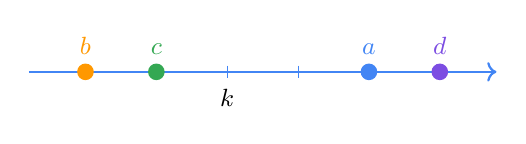
\begin{tikzpicture}[x=0.9cm]
\draw[->,thick,Navy] (-2.8,0)--(3.8,0);
\foreach \i in {-2,...,3}{\draw[Navy] (\i,0.08)--(\i,-0.08);}
\node[below,font=\small] at (0,-0.1){$k$};
\foreach \i/\l/\c in {-2/b/tmOrange,-1/c/tmGreen,2/a/tmBlue,3/d/tmPurple}{\fill[\c] (\i,0) circle (3pt); \node[above,font=\small\bfseries,text=\c] at (\i,0.1){$\l$};}
\end{tikzpicture}\end{center}
\begin{warnbox}Nhìn ``$a-2$'' có dấu trừ, nhiều bạn nghĩ $a$ nhỏ. Nhưng $a$ phải \emph{bớt đi} $2$ mới bằng $k$, nên $a$ lớn hơn $k$. Ngược lại $b$ phải \emph{thêm} $2$ mới bằng $k$, nên $b$ nhỏ hơn $k$.\end{warnbox}
\verify{Chọn thử $k=6$ (để cả bốn số đều lớn hơn $3$): $a=8$, $b=4$, $c=5$, $d=9$ (đều lớn hơn $3$). Khi đó $\dfrac{1}{8-2}=\dfrac{1}{4+2}=\dfrac{1}{5+1}=\dfrac{1}{9-3}=\dfrac{1}{6}$ và quả thật $4<5<8<9$, tức $b<c<a<d$.}
Thứ tự $b<c<a<d$ là phương án \textbf{(E)}.
\ans{(E) $b<c<a<d$}
}

% ---------------------------------------------------------------- Bài 13
\begin{probbox}{13}{\relax}
Một hình chữ nhật có chiều dài $x$ và chiều rộng $y$. Một tam giác có cạnh đáy bằng $16$ và chiều cao tương ứng bằng $x$.
Nếu diện tích hình chữ nhật bằng diện tích tam giác thì giá trị của $y$ là
\choices{$16$}{$4$}{$8$}{$12$}{$32$}
\end{probbox}
\probsol{
\textbf{Phân tích đề.} Hình chữ nhật: dài $x$, rộng $y$. Tam giác: đáy $16$, cao $x$. Hai diện tích bằng nhau. Tìm $y$
(lưu ý: đề không cho $x$, nhưng ta sẽ thấy $x$ tự ``biến mất'').
\begin{figC}
\draw[tmBlue,line width=1pt,fill=tmBlue!10] (0,0) rectangle (2.4,1.4);
\node[below] at (1.2,0){$x$}; \node[left] at (0,0.7){$y$};
\draw[tmOrange!85!black,line width=1pt,fill=tmOrange!12] (3.6,0)--(7.6,0)--(4.6,2.4)--cycle;
\draw[dashed,Slate] (4.6,2.4)--(4.6,0); \draw[Slate] (4.6,0.18)--(4.78,0.18)--(4.78,0);
\node[below] at (5.6,0){$16$}; \node[left,font=\small] at (4.6,1.1){$x$};
\end{figC}
\step{1}{Viết hai công thức diện tích}
\begin{recallbox}Diện tích hình chữ nhật $=$ dài $\times$ rộng. Diện tích tam giác $=\dfrac{\text{đáy}\times\text{chiều cao}}{2}$.\end{recallbox}
Hình chữ nhật: $S_1=x\cdot y=xy$.\quad Tam giác: $S_2=\dfrac{16\cdot x}{2}=8x$.
\step{2}{Lập phương trình và giải}
$xy=8x$. Vì $x$ là một độ dài nên $x>0$; chia cả hai vế cho $x$: $y=8$.
\begin{proofbox}Có thể hiểu không cần chia: $x\cdot y$ và $x\cdot 8$ là ``$x$ nhóm $y$'' và ``$x$ nhóm $8$''. Hai tích bằng nhau với cùng số nhóm $x\neq 0$ thì mỗi nhóm phải bằng nhau: $y=8$.\end{proofbox}
\begin{warnbox}Quên chia đôi khi tính diện tích tam giác sẽ dẫn đến $y=16$ (phương án A).\end{warnbox}
\verify{Thử $x=5$: hình chữ nhật $5\times 8=40$; tam giác $\dfrac{16\cdot 5}{2}=40$. Bằng nhau. (Với $x$ bất kì cũng đúng.)}
Vậy chọn \textbf{(C)}.
\ans{(C) $8$}
}

% ---------------------------------------------------------------- Bài 14
\begin{probbox}{14}{\relax}
Kí hiệu \aeaBox{3}{4}{5}{6} được tính theo quy tắc: $3\times 6+4\times 5=38$. Biết rằng \aeaBox{2}{6}{1}{\ } có giá trị bằng $16$.
Số cần điền vào ô trống là
\choices{$1$}{$2$}{$3$}{$4$}{$5$}
\end{probbox}
\probsol{
\textbf{Phân tích đề.} Trước hết phải hiểu quy tắc từ ví dụ đã cho, rồi áp dụng cho ô có số chưa biết.
\step{1}{Tìm quy tắc}
Trong \aeaBox{3}{4}{5}{6}: $3$ (trên trái) nhân $6$ (dưới phải), cộng với $4$ (trên phải) nhân $5$ (dưới trái): $3\times 6+4\times 5=18+20=38$.
Tức là: \emph{nhân hai số theo mỗi đường chéo rồi cộng lại}. Tổng quát, \aeaBox{a}{b}{c}{d} $=a\times d+b\times c$.
\step{2}{Đặt ẩn cho ô trống và lập phương trình}
Gọi số ở ô trống (dưới phải) là $x$. Theo quy tắc: \aeaBox{2}{6}{1}{x} $=2\times x+6\times 1=2x+6$.
Đề cho giá trị bằng $16$: $2x+6=16$.
\step{3}{Giải}
Trừ $6$ ở hai vế: $2x=10$. Chia hai vế cho $2$: $x=5$.
\verify{$2\times 5+6\times 1=10+6=16$. Đúng.}
\begin{warnbox}Đừng ghép nhầm cặp: $2\times 6+1\times x$ (nhân theo hàng) là sai quy tắc; với cách đó sẽ ra $x=4$ (phương án D). Hãy kiểm tra quy tắc với ví dụ $38$ trước khi dùng.\end{warnbox}
Vậy chọn \textbf{(E)}.
\begin{parentbox}Hãy cùng con ``sáng chế'' một kí hiệu mới (chẳng hạn nhân theo hàng rồi trừ) và đố nhau. Điều quan trọng là luôn kiểm tra quy tắc với ví dụ mẫu trước khi dùng.\end{parentbox}
\ans{(E) $5$}
}

% ---------------------------------------------------------------- Bài 15
\begin{probbox}{15}{\relax}
Người ta cân ba quả bí ngô theo từng cặp, đủ mọi cách ghép đôi. Khối lượng của các cặp lần lượt là $12$ kg, $13$ kg và $15$ kg.
Quả bí nhẹ nhất nặng bao nhiêu?
\choices{$4$ kg}{$5$ kg}{$6$ kg}{$7$ kg}{$8$ kg}
\end{probbox}
\probsol{
\textbf{Phân tích đề.} Ba quả bí ghép đôi thì có đúng $3$ cặp. Gọi khối lượng ba quả từ nhẹ đến nặng là $a\le b\le c$ (kg).
Cặp nhẹ nhất là hai quả nhẹ nhất, cặp nặng nhất là hai quả nặng nhất:
$a+b=12$, \ $a+c=13$, \ $b+c=15$.
\step{1}{Cộng cả ba cặp}
Mỗi quả có mặt trong đúng \emph{hai} cặp: $(a+b)+(a+c)+(b+c)=12+13+15=40$, tức $2(a+b+c)=40$.
\begin{recallbox}Ba vật cân từng đôi: tổng ba vật bằng một nửa tổng các kết quả cân.\end{recallbox}
\step{2}{Tổng khối lượng ba quả}
$a+b+c=40:2=20$ (kg).
\step{3}{Tìm quả nhẹ nhất}
Quả nhẹ nhất $a$ là quả \emph{không} có mặt trong cặp nặng nhất ($b+c=15$):
$a=(a+b+c)-(b+c)=20-15=5$ (kg).
(Tương tự: $b=20-13=7$ kg, \ $c=20-12=8$ kg.)
\begin{barfigC}
\blk{0}{1.25}{0}{0.5}{tmGreen}{a}
\blk{1.25}{3}{0}{0.5}{tmOrange}{b}
\brcup{0}{3}{0.5}{12 kg}
\blk{0}{1.25}{-0.9}{0.5}{tmGreen}{a}
\blk{1.25}{3.25}{-0.9}{0.5}{tmPurple}{c}
\brcdn{0}{3.25}{-1.35}{13 kg}
\end{barfigC}
\verify{$5+7=12$, \ $5+8=13$, \ $7+8=15$. Đúng cả ba cặp.}
\begin{warnbox}Đừng lấy $12:2=6$ kg và cho rằng mỗi quả trong cặp nhẹ nhất nặng $6$ kg: hai quả trong một cặp không nhất thiết nặng bằng nhau. Phương án (E) $8$ kg là quả \emph{nặng nhất}.\end{warnbox}
Quả nhẹ nhất nặng $5$ kg, ứng với phương án \textbf{(B)}.
\begin{parentbox}Cho con dùng ba đồ vật trong nhà và một chiếc cân: cân từng cặp, cộng ba kết quả rồi chia đôi, so với khi đặt cả ba lên cân. Con sẽ tự thấy vì sao phải chia $2$.\end{parentbox}
\ans{(B) $5$ kg}
}

% ---------------- part b ----------------
% ===== Topic 1, part b (VI): problems 16-30 =====
% helper shapes for the balance-scale problems (topic-specific prefix \ae...)
% \aeShp{code}{x}{y}: draw shape (T triangle, C circle, S square, D diamond, Q question mark) with lower-left corner at (x,y)
\providecommand{\aeShp}[3]{%
  \if#1T\draw[tmBlue!80!black,line width=0.8pt,fill=tmBlue!18] (#2,#3)--(#2+0.34,#3)--(#2+0.17,#3+0.3)--cycle;\fi
  \if#1C\draw[tmOrange!85!black,line width=0.8pt,fill=tmOrange!22] (#2+0.15,#3+0.15) circle (0.15);\fi
  \if#1S\draw[tmGreen!80!black,line width=0.8pt,fill=tmGreen!18] (#2,#3) rectangle (#2+0.3,#3+0.3);\fi
  \if#1D\draw[tmPurple!85!black,line width=0.8pt,fill=tmPurple!18] (#2+0.13,#3)--(#2+0.26,#3+0.16)--(#2+0.13,#3+0.32)--(#2,#3+0.16)--cycle;\fi
  \if#1Q\node[font=\Large\bfseries,text=Ink,inner sep=0pt,anchor=south] at (#2+0.15,#3) {?};\fi}
\providecommand{\aeTri}{\tikz[baseline=0pt]{\aeShp{T}{0}{0}}}
\providecommand{\aeCir}{\tikz[baseline=0pt]{\aeShp{C}{0}{0}}}
\providecommand{\aeSq}{\tikz[baseline=0pt]{\aeShp{S}{0}{0}}}
\providecommand{\aeDia}{\tikz[baseline=0pt]{\aeShp{D}{0}{0}}}
% \aeRow{list}{xcentre}{y}: a row of shapes (e.g. {T,C}) centred at xcentre, standing on height y
\providecommand{\aeRow}[3]{%
  \foreach \aeS [count=\aeI] in {#1}{\xdef\aeN{\aeI}}%
  \foreach \aeS [count=\aeI] in {#1}{\aeShp{\aeS}{#2-0.19*\aeN+0.38*\aeI-0.36}{#3+0.03}}}
% \aeScale{x}{y}{left list}{right list}: a balanced scale centred at (x,y)
\providecommand{\aeScale}[4]{\begin{scope}[shift={(#1,#2)}]
  \draw[Ink,line width=1pt] (-1.9,0.55)--(-0.5,0.55) (-1.2,0.55)--(-1.2,0.25)--(1.2,0.25)--(1.2,0.55) (0.5,0.55)--(1.9,0.55);
  \draw[Ink,line width=0.9pt,fill=Ink!12] (-0.2,-0.12)--(0,0.25)--(0.2,-0.12)--cycle;
  \aeRow{#3}{-1.2}{0.55}\aeRow{#4}{1.2}{0.55}
\end{scope}}

% ------------------------------------------------------------------ 16
\begin{probbox}{16}{\relax}
Bạn Hồng đang tập tiết kiệm. Hôm nay trong tài khoản của Hồng có $120$ nghìn đồng. Từ nay, mỗi lần gửi tiết kiệm Hồng sẽ gửi thêm đúng $30$ nghìn đồng. Nếu Hồng gửi $m$ lần như vậy thì biểu thức nào dưới đây biểu thị đúng số tiền (tính bằng nghìn đồng) có trong tài khoản?
\choices{$120+m$}{$30m$}{$30+120m$}{$150m$}{$120+30m$}
\end{probbox}
\probsol{
\textbf{Phân tích đề.} Cho biết: lúc đầu có $120$ nghìn đồng; mỗi lần gửi thêm $30$ nghìn đồng; gửi $m$ lần. Cần tìm: biểu thức đại số cho tổng số tiền sau $m$ lần gửi.

\step{1}{Thử với vài giá trị cụ thể của $m$ để thấy quy luật}
\begin{center}
\begin{tabular}{|c|c|c|}
\hline
\rowcolor{tmBlue!10}\textbf{Số lần gửi} & \textbf{Số tiền gửi thêm} & \textbf{Tổng số tiền (nghìn đồng)}\\ \hline
$0$ & $0$ & $120$\\ \hline
$1$ & $30$ & $120+30=150$\\ \hline
$2$ & $30+30=30\cdot 2=60$ & $120+60=180$\\ \hline
$3$ & $30\cdot 3=90$ & $120+90=210$\\ \hline
$m$ & $30\cdot m=30m$ & $120+30m$\\ \hline
\end{tabular}
\end{center}

\step{2}{Viết biểu thức}
Số tiền \emph{gửi thêm} sau $m$ lần là $m$ lần của $30$, tức là $30m$. Cộng với số tiền có sẵn $120$, ta được
\[ \text{Tổng số tiền} = 120 + 30m \ \text{(nghìn đồng)}. \]
\begin{recallbox}$30m$ nghĩa là $30\cdot m$ (ta được phép bỏ dấu nhân giữa một số và một chữ). Cộng một số $a$ lặp lại $m$ lần thì được $a\cdot m$.\end{recallbox}

\step{3}{Loại các phương án sai}
\begin{itemize}[leftmargin=1.3em,itemsep=1pt]
\item (A) $120+m$: chỉ cộng thêm $1$ nghìn mỗi lần -- sai.
\item (B) $30m$: quên mất $120$ nghìn có sẵn. Với $m=0$ cho $0$ -- sai.
\item (C) $30+120m$: đảo vai trò hai số. Với $m=1$ cho $150$ (trùng!) nhưng với $m=2$ cho $270\ne 180$ -- sai.
\item (D) $150m$: với $m=2$ cho $300\ne 180$ -- sai.
\end{itemize}
\begin{warnbox}Thử với \emph{một} giá trị $m=1$ là chưa đủ: cả (C), (D) và (E) đều cho $150$. Hãy thử thêm $m=0$ hoặc $m=2$ để phân biệt.\end{warnbox}
\verify{Với $m=3$: $120+30\cdot 3=210$, đúng như bảng ở Bước 1.}
Vậy chọn \textbf{(E)}.
\ans{(E) $120+30m$}
}

% ------------------------------------------------------------------ 17
\begin{probbox}{17}{\relax}
Cả bốn chiếc cân dưới đây đều đang thăng bằng. Các hình giống nhau có khối lượng bằng nhau. Một cách có thể thay vào dấu ``?'' để chiếc cân thứ tư thăng bằng là
\begin{figC}
\aeScale{0}{1.6}{T,C}{S}
\aeScale{4.6}{1.6}{T}{D,C}
\aeScale{0}{0}{D,T}{C,S}
\aeScale{4.6}{0}{C,D,T}{Q}
\node[font=\footnotesize\bfseries,text=Slate] at (-2.25,2.45) {1};
\node[font=\footnotesize\bfseries,text=Slate] at (2.35,2.45) {2};
\node[font=\footnotesize\bfseries,text=Slate] at (-2.25,0.85) {3};
\node[font=\footnotesize\bfseries,text=Slate] at (2.35,0.85) {4};
\end{figC}
\choices{\aeTri\,\aeSq}{\aeDia\,\aeTri}{\aeCir\,\aeSq}{\aeSq\,\aeDia}{\aeTri\,\aeCir}
\end{probbox}
\probsol{
\textbf{Phân tích đề.} Mỗi chiếc cân thăng bằng cho ta một \emph{đẳng thức}: tổng khối lượng đĩa trái bằng tổng khối lượng đĩa phải. Ta viết thẳng các hình vào đẳng thức (mỗi hình thay cho khối lượng của nó):
\[
\text{Cân 1: } \aeTri+\aeCir=\aeSq,\qquad
\text{Cân 2: } \aeTri=\aeDia+\aeCir,\qquad
\text{Cân 3: } \aeDia+\aeTri=\aeCir+\aeSq.
\]
Cần tìm: đĩa phải của cân 4 phải nặng bằng $\aeCir+\aeDia+\aeTri$. Ý tưởng: đổi mọi hình về cùng một ``đơn vị'' là \aeCir.
\begin{recallbox}Nếu cân thăng bằng thì khi \emph{thay} một vật bằng các vật nặng bằng nó, hoặc \emph{bỏ bớt} những vật giống nhau ở cả hai đĩa, cân vẫn thăng bằng. Đây chính là tính chất của đẳng thức: $a=b \Rightarrow a+c=b+c$ và $a-c=b-c$.\end{recallbox}

\step{1}{Dùng cân 2 để thay \aeTri\ trong cân 1}
Theo cân 2, $\aeTri=\aeDia+\aeCir$. Thay vào cân 1:
\[ \aeSq=\aeTri+\aeCir=(\aeDia+\aeCir)+\aeCir=\aeDia+2\,\aeCir. \]

\step{2}{Thay vào cân 3 để tìm \aeDia}
Đĩa trái cân 3: $\aeDia+\aeTri=\aeDia+(\aeDia+\aeCir)=2\,\aeDia+\aeCir$.\par
Đĩa phải cân 3: $\aeCir+\aeSq=\aeCir+(\aeDia+2\,\aeCir)=\aeDia+3\,\aeCir$.\par
Vậy $2\,\aeDia+\aeCir=\aeDia+3\,\aeCir$. Bỏ bớt một \aeDia\ và một \aeCir\ ở cả hai đĩa:
\[ \aeDia = 2\,\aeCir. \]

\step{3}{Đổi mọi hình về đơn vị \aeCir}
\[ \aeDia=2\,\aeCir,\qquad \aeTri=\aeDia+\aeCir=3\,\aeCir,\qquad \aeSq=\aeDia+2\,\aeCir=4\,\aeCir. \]
Đĩa trái cân 4: $\aeCir+\aeDia+\aeTri=1+2+3=6$ (\aeCir).

\step{4}{Tính từng phương án (theo đơn vị \aeCir)}
\begin{center}
\begin{tabular}{|c|c|c|c|c|c|}
\hline
\rowcolor{tmBlue!10} & (A) \aeTri\,\aeSq & (B) \aeDia\,\aeTri & (C) \aeCir\,\aeSq & (D) \aeSq\,\aeDia & (E) \aeTri\,\aeCir\\ \hline
Khối lượng & $3+4=7$ & $2+3=5$ & $1+4=5$ & $4+2=\mathbf{6}$ & $3+1=4$\\ \hline
\end{tabular}
\end{center}
Chỉ có (D) nặng đúng $6$ \aeCir.
\verify{Lấy \aeCir\ nặng $1$~kg thì \aeDia, \aeTri, \aeSq\ nặng $2$, $3$, $4$~kg. Cân 1: $3+1=4$ \checkmark; cân 2: $3=2+1$ \checkmark; cân 3: $2+3=1+4$ \checkmark; cân 4: $1+2+3=6=4+2$ \checkmark.}
\begin{tipbox}Khi có nhiều ẩn, hãy chọn \emph{một} hình làm đơn vị đo và biểu diễn mọi hình khác theo nó -- giống như đổi mọi số tiền ra cùng một loại tờ tiền.\end{tipbox}
Vậy chọn \textbf{(D)}.
\ans{(D) \aeSq\,\aeDia}
}

% ------------------------------------------------------------------ 18
\begin{probbox}{18}{\relax}
Số cần điền vào ô trống để có đẳng thức đúng $\dfrac{3}{7}=\dfrac{\square}{63}$ là
\choices{$27$}{$9$}{$59$}{$63$}{$3$}
\end{probbox}
\probsol{
\textbf{Phân tích đề.} Hai phân số bằng nhau, đã biết mẫu của phân số thứ hai là $63$. Cần tìm tử số.
\begin{recallbox}\textbf{Tính chất cơ bản của phân số:} nếu nhân cả tử và mẫu của một phân số với cùng một số khác $0$ thì được một phân số bằng nó: $\dfrac{a}{b}=\dfrac{a\cdot k}{b\cdot k}$ $(k\ne 0)$.\end{recallbox}

\step{1}{Mẫu số đã được nhân với bao nhiêu?}
Từ $7$ lên $63$: $63:7=9$. Vậy mẫu số đã được nhân với $9$.

\step{2}{Nhân tử số với cùng số đó}
Để phân số không đổi, tử số cũng phải nhân với $9$: $3\cdot 9=27$.
\[ \frac{3}{7}=\frac{3\cdot 9}{7\cdot 9}=\frac{27}{63}. \]

\step{3}{Cách khác: dùng ``tích chéo''}
Hai phân số $\dfrac{a}{b}=\dfrac{c}{d}$ khi và chỉ khi $a\cdot d=b\cdot c$. Gọi số cần điền là $x$: $3\cdot 63=7\cdot x$, tức $189=7x$, nên $x=189:7=27$.
\begin{warnbox}Một số bạn thấy $63-7=56$ rồi lấy $3+56=59$ (phương án C). Phân số không thay đổi khi \emph{cộng} cùng một số vào tử và mẫu! Phải \emph{nhân} (hoặc chia).\end{warnbox}
\verify{$27:63$ rút gọn cho $9$ được $3:7$, tức $\dfrac{27}{63}=\dfrac{3}{7}$ \checkmark.}
Vậy chọn \textbf{(A)}.
\ans{(A) $27$}
}

% ------------------------------------------------------------------ 19
\begin{probbox}{19}{\relax}
Tổng của bốn số bằng $T$. Mỗi số trong bốn số đó được tăng thêm $1$ đơn vị. Cộng bốn số mới lại, rồi nhân tổng vừa được với $3$. Kết quả cuối cùng bằng
\choices{$3T+3$}{$3T+4$}{$3T+12$}{$T+12$}{$12T$}
\end{probbox}
\probsol{
\textbf{Phân tích đề.} Bốn số chưa biết, chỉ biết tổng của chúng là $T$. Ta không cần biết từng số -- chỉ cần theo dõi \emph{tổng} thay đổi thế nào.

\step{1}{Đặt tên các số}
Gọi bốn số là $a$, $b$, $c$, $d$. Theo đề: $a+b+c+d=T$.

\step{2}{Tăng mỗi số thêm 1 rồi cộng lại}
Bốn số mới là $a+1$, $b+1$, $c+1$, $d+1$. Tổng của chúng:
\[ (a+1)+(b+1)+(c+1)+(d+1)=(a+b+c+d)+(1+1+1+1)=T+4. \]
\begin{recallbox}Phép cộng có tính chất giao hoán và kết hợp, nên ta được phép nhóm các chữ với nhau và các số với nhau.\end{recallbox}

\step{3}{Nhân với 3}
\[ 3\cdot(T+4)=3\cdot T+3\cdot 4=3T+12. \]
\begin{recallbox}\textbf{Tính chất phân phối:} $k\cdot(x+y)=k\cdot x+k\cdot y$. Phải nhân $3$ với \emph{từng} số hạng trong ngoặc.\end{recallbox}
\begin{warnbox}Hai lỗi hay gặp: (1) chỉ cộng $1$ vào tổng (thay vì $4$, vì có bốn số) rồi được $3T+3$; (2) quên nhân $3$ với số $4$ rồi được $3T+4$.\end{warnbox}
\verify{Lấy bốn số $1,2,3,4$: $T=10$. Số mới $2,3,4,5$ có tổng $14$; nhân $3$ được $42$. Còn $3T+12=30+12=42$ \checkmark. Các phương án khác cho $33$, $34$, $22$, $120$ -- đều sai.}
Vậy chọn \textbf{(C)}.
\ans{(C) $3T+12$}
}

% ------------------------------------------------------------------ 20
\begin{probbox}{20}{\relax}
Hai tam giác cân, mỗi tam giác đều có ít nhất một góc bằng $70^\circ$. Ở tam giác thứ nhất, số đo (theo độ) của mỗi góc trong hai góc còn lại là số chẵn. Ở tam giác thứ hai, số đo của mỗi góc trong hai góc còn lại là số lẻ. Gọi $S$ là tổng hai góc bằng nhau của tam giác thứ nhất và $T$ là tổng hai góc bằng nhau của tam giác thứ hai. Giá trị của $S+T$ là
\choices{$280^\circ$}{$250^\circ$}{$220^\circ$}{$200^\circ$}{$300^\circ$}
\end{probbox}
\probsol{
\textbf{Phân tích đề.} Một tam giác cân có hai góc ở đáy bằng nhau. Góc $70^\circ$ có thể là \emph{góc ở đỉnh} hoặc \emph{góc ở đáy}. Ta xét cả hai khả năng, rồi xem khả năng nào cho ``hai góc còn lại chẵn'', khả năng nào cho ``hai góc còn lại lẻ''.
\begin{recallbox}Tổng ba góc trong một tam giác bằng $180^\circ$. Trong tam giác cân, hai góc ở đáy bằng nhau.\end{recallbox}

\step{1}{Khả năng 1: góc $70^\circ$ là góc ở đáy}
Khi đó góc ở đáy còn lại cũng bằng $70^\circ$. Góc ở đỉnh bằng $180^\circ-70^\circ-70^\circ=40^\circ$.\par
Ba góc: $70^\circ,\ 70^\circ,\ 40^\circ$. Hai góc còn lại (ngoài một góc $70^\circ$) là $70^\circ$ và $40^\circ$ -- \textbf{đều chẵn}.

\step{2}{Khả năng 2: góc $70^\circ$ là góc ở đỉnh}
Hai góc ở đáy bằng nhau và có tổng $180^\circ-70^\circ=110^\circ$, nên mỗi góc bằng $110^\circ:2=55^\circ$.\par
Ba góc: $70^\circ,\ 55^\circ,\ 55^\circ$. Hai góc còn lại là $55^\circ$ và $55^\circ$ -- \textbf{đều lẻ}.
\begin{figC}
\begin{scope}
\draw[tmBlue,line width=1.1pt,fill=tmBlue!8] (0,0)--(1.6,0)--(0.8,2.2)--cycle;
\node[font=\scriptsize] at (0.33,0.2) {$70^\circ$};
\node[font=\scriptsize] at (1.27,0.2) {$70^\circ$};
\node[font=\scriptsize] at (0.8,1.65) {$40^\circ$};
\node[font=\footnotesize\bfseries,text=tmBlue] at (0.8,-0.35) {Tam giác thứ nhất};
\end{scope}
\begin{scope}[xshift=3.6cm]
\draw[tmOrange,line width=1.1pt,fill=tmOrange!8] (0,0)--(2.4,0)--(1.2,1.71)--cycle;
\node[font=\scriptsize] at (0.45,0.18) {$55^\circ$};
\node[font=\scriptsize] at (1.95,0.18) {$55^\circ$};
\node[font=\scriptsize] at (1.2,1.25) {$70^\circ$};
\node[font=\footnotesize\bfseries,text=tmOrange!85!black] at (1.2,-0.35) {Tam giác thứ hai};
\end{scope}
\end{figC}

\step{3}{Xác định $S$ và $T$}
Tam giác thứ nhất (hai góc còn lại chẵn) là khả năng 1. Hai góc \emph{bằng nhau} của nó là hai góc $70^\circ$: $S=70^\circ+70^\circ=140^\circ$.\par
Tam giác thứ hai (hai góc còn lại lẻ) là khả năng 2. Hai góc bằng nhau là hai góc $55^\circ$: $T=55^\circ+55^\circ=110^\circ$.

\step{4}{Tính $S+T$}
$S+T=140^\circ+110^\circ=250^\circ$.
\begin{warnbox}``Tổng hai góc bằng nhau'' là tổng hai góc \emph{ở đáy}, không phải tổng hai góc ``còn lại''. Ở tam giác thứ nhất, hai góc còn lại là $70^\circ$ và $40^\circ$ (tổng $110^\circ$), nhưng hai góc bằng nhau là $70^\circ$ và $70^\circ$ (tổng $140^\circ$). Nhầm chỗ này sẽ ra $110^\circ+110^\circ=220^\circ$ (phương án C).\end{warnbox}
\verify{$70+70+40=180$ và $70+55+55=180$ \checkmark.}
Vậy chọn \textbf{(B)}.
\ans{(B) $250^\circ$}
}

% ------------------------------------------------------------------ 21
\begin{probbox}{21}{\relax}
Bạn Ánh tham gia một chuyến chèo thuyền kayak kéo dài $6$ ngày với tổng quãng đường $168$~km. Vừa hết ngày thứ ba, Ánh đã đi được $\frac{3}{7}$ tổng quãng đường. Trong những ngày còn lại, trung bình mỗi ngày Ánh phải chèo bao nhiêu ki-lô-mét?
\choices{$29$}{$24$}{$27$}{$32$}{$26$}
\end{probbox}
\probsol{
\textbf{Phân tích đề.} Cho biết: tổng quãng đường $168$~km; chuyến đi $6$ ngày; sau $3$ ngày đã đi $\frac{3}{7}$ quãng đường. Cần tìm: số km trung bình mỗi ngày trong số ngày còn lại.
\begin{recallbox}Muốn tìm $\frac{m}{n}$ của một số, ta nhân số đó với $\frac{m}{n}$ (chia cho $n$ rồi nhân với $m$).\end{recallbox}

\step{1}{Vẽ sơ đồ: chia quãng đường thành 7 phần bằng nhau}
\begin{barfigC}
\foreach \i in {0,1,2}{\blk{\i*1.3}{\i*1.3+1.3}{0}{0.6}{tmGreen}{}}
\foreach \i in {3,4,5,6}{\blk{\i*1.3}{\i*1.3+1.3}{0}{0.6}{tmOrange}{}}
\brcup{0}{3.9}{0.55}{đã đi: $3$ phần (3 ngày)}
\brcup{3.9}{9.1}{0.55}{còn lại: $4$ phần (3 ngày)}
\brcdn{0}{9.1}{-0.55}{$168$ km}
\end{barfigC}
Mỗi phần dài $168:7=24$ (km).

\step{2}{Tính quãng đường đã đi và còn lại}
Đã đi: $3$ phần $=3\cdot 24=72$ (km).\par
Còn lại: $168-72=96$ (km) (hoặc $4$ phần $=4\cdot 24=96$~km).

\step{3}{Số ngày còn lại}
Chuyến đi $6$ ngày, đã xong $3$ ngày, nên còn $6-3=3$ ngày.

\step{4}{Trung bình mỗi ngày}
$96:3=32$ (km/ngày).
\begin{warnbox}Đừng nhầm ``phần quãng đường còn lại'' ($\frac{4}{7}$) với ``số ngày còn lại'' ($3$ ngày). Phương án (B) $24$~km chỉ là độ dài của \emph{một phần bảy} quãng đường.\end{warnbox}
\verify{$72+3\cdot 32=72+96=168$~km \checkmark.}
Vậy chọn \textbf{(D)}.
\ans{(D) $32$~km mỗi ngày}
}

% ------------------------------------------------------------------ 22
\begin{probbox}{22}{\stars{1}}
Một chấm tròn xuất phát tại điểm $(20;19)$ trên mặt phẳng tọa độ. Ở bước thứ nhất, chấm di chuyển $1$ đơn vị theo phương ngang hoặc phương dọc, tức là đến một trong các điểm $(21;19)$, $(19;19)$, $(20;20)$ hoặc $(20;18)$. Ở bước thứ hai, chấm di chuyển $2$ đơn vị (về chiều nào cũng được) theo phương \emph{vuông góc} với bước thứ nhất. Từ đó về sau, mỗi bước dài hơn bước trước $1$ đơn vị ($3$ đơn vị, $4$ đơn vị, $5$ đơn vị, \dots) và luôn vuông góc với bước ngay trước nó. Chấm dừng lại sau $10$ bước. Điểm nào dưới đây \textbf{không thể} là vị trí cuối cùng của chấm?
\choices{$(27;33)$}{$(30;40)$}{$(21;21)$}{$(42;44)$}{$(37;37)$}
\end{probbox}
\probsol{
\textbf{Phân tích đề.} Các bước có độ dài $1,2,3,\dots,10$. ``Vuông góc với bước trước'' nghĩa là các bước \emph{luân phiên} ngang -- dọc -- ngang -- dọc\dots\ Ta cần tìm điểm mà chấm không bao giờ tới được.
\begin{recallbox}Trên mặt phẳng tọa độ, đi sang phải (trái) $k$ đơn vị làm hoành độ (số thứ nhất) tăng (giảm) $k$; đi lên (xuống) $k$ đơn vị làm tung độ (số thứ hai) tăng (giảm) $k$.\end{recallbox}

\step{1}{Tách các bước thành hai nhóm}
Nếu bước $1$ là bước ngang thì các bước ngang là bước $1,3,5,7,9$ (độ dài lẻ) và các bước dọc là bước $2,4,6,8,10$ (độ dài chẵn). Nếu bước $1$ là bước dọc thì ngược lại.\par
Mỗi bước có thể đi theo chiều dương (dấu $+$) hoặc chiều âm (dấu $-$). Vậy độ dịch chuyển theo một phương là
\[ \pm 1\pm 3\pm 5\pm 7\pm 9 \quad\text{(nhóm lẻ)},\qquad \pm 2\pm 4\pm 6\pm 8\pm 10\quad\text{(nhóm chẵn).} \]

\step{2}{Nhóm lẻ cho được những số nào?}
Nếu tất cả mang dấu $+$: $1+3+5+7+9=25$. Khi đổi dấu một bước độ dài $a$ từ $+$ sang $-$, tổng giảm đi $2a$ (mất $a$ và còn bị trừ thêm $a$). Vậy:
\[ \text{độ dịch chuyển}=25-2\times(\text{tổng các độ dài bị đổi dấu}). \]
Muốn được $21$, cần tổng các độ dài bị đổi dấu là $(25-21):2=2$. Nhưng trong $\{1,3,5,7,9\}$ không có cách chọn nào có tổng bằng $2$ (chọn $1$ thì được $1$; chọn thêm bất kỳ số nào thì đã $\ge 4$). Vậy \textbf{nhóm lẻ không thể cho độ dịch chuyển $21$} (tương tự cũng không thể cho $-21$).
\begin{proofbox}Mọi tổng con của $\{1,3,5,7,9\}$ có thể bằng: $0,1,3,4,5,6,7,8,9,\dots$ nhưng \emph{không} bằng $2$, vì số nhỏ nhất là $1$, số nhỏ thứ hai là $3$, nên chọn từ hai số trở lên thì tổng ít nhất $1+3=4$.\end{proofbox}

\step{3}{Kiểm tra phương án (B) $(30;40)$}
Độ dịch chuyển: ngang $30-20=10$, dọc $40-19=21$.\par
Một tổng có dấu của $5$ số lẻ luôn là số \emph{lẻ}; của các số chẵn luôn là số \emph{chẵn}. Vì $21$ lẻ nên phương dọc phải là nhóm lẻ, tức phải có $\pm1\pm3\pm5\pm7\pm9=21$ -- điều này không thể theo Bước 2. Vậy chấm \textbf{không thể} đến $(30;40)$.

\step{4}{Các phương án còn lại đều đến được (chỉ ra cách đi)}
\begin{center}\small
\begin{tabular}{|c|c|c|c|}
\hline
\rowcolor{tmBlue!10}\textbf{Điểm} & \textbf{Dịch chuyển (ngang; dọc)} & \textbf{Nhóm lẻ} & \textbf{Nhóm chẵn}\\ \hline
(A) $(27;33)$ & $(7;14)$ & $1+3+5+7-9=7$ & $2+4+6-8+10=14$\\ \hline
(C) $(21;21)$ & $(1;2)$ & $1-3+5+7-9=1$ & $2-4+6+8-10=2$\\ \hline
(D) $(42;44)$ & $(22;25)$ & $1+3+5+7+9=25$ & $2-4+6+8+10=22$\\ \hline
(E) $(37;37)$ & $(17;18)$ & $-1-3+5+7+9=17$ & $2+4-6+8+10=18$\\ \hline
\end{tabular}
\end{center}
(Ở (D), độ dịch chuyển ngang $22$ là số chẵn nên bước đầu tiên phải là bước dọc.) Ví dụ đường đi tới $(21;21)$: các bước lần lượt là phải $1$, lên $2$, trái $3$, xuống $4$, phải $5$, lên $6$, phải $7$, lên $8$, trái $9$, xuống $10$:
\begin{figC}\begin{scope}[scale=0.24]
\draw[Line,line width=0.3pt] (-3,-3) grid (11,13);
\draw[tmBlue,line width=1.2pt,->] (0,0)--(1,0)--(1,2)--(-2,2)--(-2,-2)--(3,-2)--(3,4)--(10,4)--(10,12)--(1,12)--(1,2);
\fill[tmGreen] (0,0) circle (7pt); \fill[AnsRed] (1,2) circle (7pt);
\node[font=\scriptsize,anchor=north east] at (0,0) {$(20;19)$};
\node[font=\scriptsize,anchor=west,fill=white,inner sep=1pt] at (1.6,1.1) {$(21;21)$};
\end{scope}\end{figC}
\begin{warnbox}Chỉ xét tính chẵn -- lẻ là chưa đủ: cả $10$ (chẵn) và $21$ (lẻ) đều ``hợp lệ'' về tính chẵn lẻ, nhưng $21$ vẫn không đạt được. Phải kiểm tra thật sự xem có cách chọn dấu hay không.\end{warnbox}
Vậy chọn \textbf{(B)}.
\ans{(B) $(30;40)$}
}

% ------------------------------------------------------------------ 23
\begin{probbox}{23}{\relax}
Chị Giang làm nhân viên phục vụ ở một nhà hàng. Hôm thứ Bảy, chị dậy lúc $6$\,h\,$30$ sáng, bắt đầu làm việc lúc $x$ giờ sáng và kết thúc lúc $x$ giờ chiều (cùng ngày). Hôm thứ Bảy chị Giang làm việc trong bao lâu?
\choicesII{$24-2x$ giờ}{$12-x$ giờ}{$2x$ giờ}{$0$ giờ}{$12$ giờ}
\end{probbox}
\probsol{
\textbf{Phân tích đề.} Bắt đầu lúc $x$ giờ sáng, kết thúc lúc $x$ giờ chiều. Cần tìm thời gian làm việc. Giờ dậy $6$\,h\,$30$ là thông tin \emph{thừa}, không dùng đến.
\begin{recallbox}$x$ giờ chiều (theo cách nói 12 giờ) chính là $(x+12)$ giờ theo cách tính 24 giờ. Ví dụ: $3$ giờ chiều là $15$ giờ.\end{recallbox}

\step{1}{Đổi sang cách tính 24 giờ}
Bắt đầu: $x$ giờ. Kết thúc: $x+12$ giờ.

\step{2}{Tính thời gian làm việc}
Thời gian $=$ giờ kết thúc $-$ giờ bắt đầu $=(x+12)-x=12$ (giờ).

\step{3}{Cách nghĩ khác (chia làm hai đoạn)}
\begin{figC}
\draw[Navy,line width=1pt,->] (0,0)--(8.4,0);
\foreach \x/\l in {0/{$x$ giờ sáng},4/{$12$ giờ trưa},8/{$x$ giờ chiều}}{\draw[Navy,line width=1pt] (\x,0.12)--(\x,-0.12); \node[below,font=\footnotesize] at (\x,-0.12) {\l};}
\brcup{0}{4}{0.25}{$12-x$ giờ}
\brcup{4}{8}{0.25}{$x$ giờ}
\end{figC}
Từ $x$ giờ sáng đến $12$ giờ trưa là $12-x$ giờ; từ $12$ giờ trưa đến $x$ giờ chiều là $x$ giờ. Tổng: $(12-x)+x=12$ giờ. Kết quả không phụ thuộc vào $x$!
\begin{warnbox}Phương án (B) $12-x$ chỉ là phần buổi sáng. Phương án (D) $0$ giờ xuất hiện khi lấy $x-x$ mà quên rằng một bên là ``sáng'', một bên là ``chiều''.\end{warnbox}
\verify{Nếu $x=8$: chị làm từ $8$ giờ sáng đến $8$ giờ tối ($20$ giờ), tức $20-8=12$ giờ \checkmark.}
Vậy chọn \textbf{(E)}.
\ans{(E) $12$ giờ}
}

% ------------------------------------------------------------------ 24
\begin{probbox}{24}{\stars{1}}
Một hình hộp chữ nhật kích thước $8\times 8\times n$ ($n$ là số nguyên dương) được ghép từ các hình lập phương nhỏ kích thước $1\times1\times1$. Gọi $A$ là diện tích toàn phần của hình hộp chữ nhật và $B$ là tổng diện tích toàn phần của tất cả các hình lập phương nhỏ tạo nên nó. Tổng tất cả các giá trị của $n$ để $\dfrac{B}{A}$ là một số nguyên bằng
\choices{$86$}{$90$}{$70$}{$78$}{$96$}
\end{probbox}
\probsol{
\textbf{Phân tích đề.} Cần viết $A$ và $B$ theo $n$, lập tỉ số $\frac{B}{A}$, rồi tìm mọi $n$ nguyên dương làm tỉ số này là số nguyên, cuối cùng cộng các $n$ đó lại.
\begin{figC}\begin{scope}[scale=0.8]
\draw[tmBlue,line width=1pt,fill=tmBlue!10] (0,0) rectangle (2.4,1.6);
\draw[tmBlue,line width=1pt,fill=tmBlue!20] (0,1.6)--(0.9,2.3)--(3.3,2.3)--(2.4,1.6)--cycle;
\draw[tmBlue,line width=1pt,fill=tmBlue!5] (2.4,0)--(3.3,0.7)--(3.3,2.3)--(2.4,1.6)--cycle;
\node[below,font=\footnotesize] at (1.2,0) {$8$};
\node[right,font=\footnotesize] at (3.3,1.5) {$n$};
\node[below right,font=\footnotesize] at (2.8,0.4) {$8$};
\end{scope}\end{figC}
\begin{recallbox}Hình hộp chữ nhật có ba kích thước $a,b,c$ có diện tích toàn phần (tổng diện tích $6$ mặt) là $2(ab+bc+ca)$. Hình lập phương cạnh $1$ có $6$ mặt, mỗi mặt diện tích $1$, nên diện tích toàn phần là $6$. Hình hộp $a\times b\times c$ ghép từ $a\cdot b\cdot c$ hình lập phương đơn vị.\end{recallbox}

\step{1}{Tính $A$}
$A=2(8\cdot 8+8\cdot n+8\cdot n)=2(64+16n)=128+32n$.

\step{2}{Tính $B$}
Số hình lập phương nhỏ: $8\cdot 8\cdot n=64n$. Mỗi hình có diện tích toàn phần $6$, nên $B=6\cdot 64n=384n$.

\step{3}{Rút gọn tỉ số}
\[ \frac{B}{A}=\frac{384n}{128+32n}=\frac{32\cdot 12n}{32\cdot(4+n)}=\frac{12n}{n+4}. \]

\step{4}{Tách phần nguyên}
\[ \frac{12n}{n+4}=\frac{12(n+4)-48}{n+4}=12-\frac{48}{n+4}. \]
\begin{proofbox}$12(n+4)-48=12n+48-48=12n$, nên tử số không đổi. Do đó $\frac{12n}{n+4}$ là số nguyên khi và chỉ khi $\frac{48}{n+4}$ là số nguyên, tức là $n+4$ là ước của $48$.\end{proofbox}

\step{5}{Tìm các giá trị của $n$}
Các ước dương của $48$: $1,2,3,4,6,8,12,16,24,48$. Vì $n\ge 1$ nên $n+4\ge 5$; chỉ giữ lại $6,8,12,16,24,48$:
\begin{center}
\begin{tabular}{|c|c|c|c|c|c|c|}
\hline
\rowcolor{tmBlue!10}$n+4$ & $6$ & $8$ & $12$ & $16$ & $24$ & $48$\\ \hline
$n$ & $2$ & $4$ & $8$ & $12$ & $20$ & $44$\\ \hline
$\frac{B}{A}=12-\frac{48}{n+4}$ & $4$ & $6$ & $8$ & $9$ & $10$ & $11$\\ \hline
\end{tabular}
\end{center}

\step{6}{Cộng các giá trị}
$2+4+8+12+20+44=90$.
\begin{warnbox}Đừng quên điều kiện $n\ge 1$: các ước $1,2,3,4$ của $48$ cho $n+4\le 4$, tức $n\le 0$ -- bị loại.\end{warnbox}
\verify{Với $n=2$: $A=128+64=192$, $B=768$, $\frac{B}{A}=4$ \checkmark. Với $n=44$: $A=128+1408=1536$, $B=16\,896$, $\frac{B}{A}=11$ \checkmark.}
Vậy chọn \textbf{(B)}.
\ans{(B) $90$}
}

% ------------------------------------------------------------------ 25
\begin{probbox}{25}{\stars{1}}
Ba tuyến xe buýt cắt nhau tại bến $X$ như hình vẽ (các đoạn có cùng số vạch thì dài bằng nhau). Cứ $12$ phút, xe A đi hết một lượt $P\to X\to S\to X\to P$. Cứ $20$ phút, xe B đi hết một lượt $Q\to X\to T\to X\to Q$. Cứ $28$ phút, xe C đi hết một lượt $R\to X\to U\to X\to R$. Lúc $13$\,h\,$00$, ba xe A, B, C lần lượt xuất phát từ $P$, $Q$, $R$; mỗi xe chạy với vận tốc không đổi và quay đầu ngay lập tức khi tới cuối tuyến. Các xe chạy liên tục đến $23$\,h\,$00$. Trong khoảng thời gian từ $17$\,h\,$00$ đến $22$\,h\,$00$, có bao nhiêu thời điểm mà có từ hai xe trở lên cùng có mặt tại $X$?
\begin{figC}
\draw[Ink,line width=1pt] (0,1.6)--(0,-1.6) (-2.2,0)--(2.2,0) (-1.9,-1.4)--(1.9,1.4);
\foreach \p/\q/\l/\a in {(0,1.6)/P/P/above,(0,-1.6)/S/S/below,(-2.2,0)/Q/Q/left,(2.2,0)/T/T/right,(-1.9,-1.4)/R/R/below left,(1.9,1.4)/U/U/above right}{\fill[Ink] \p circle (2pt); \node[\a,font=\small\itshape] at \p {$\l$};}
\fill[Ink] (0,0) circle (2pt); \node[below right,font=\small\itshape] at (0.05,-0.05) {$X$};
% single ticks on PX and XS
\draw[tmBlue,line width=1pt] (-0.12,0.8)--(0.12,0.8) (-0.12,-0.8)--(0.12,-0.8);
% double ticks on QX and XT
\foreach \x in {-1.1,1.1}{\draw[tmOrange,line width=1pt] (\x-0.05,-0.12)--(\x-0.05,0.12) (\x+0.05,-0.12)--(\x+0.05,0.12);}
% triple ticks on RX and XU
\foreach \t in {-0.5,0.5}{\begin{scope}[shift={(1.9*\t,1.4*\t)},rotate=36.4]
  \draw[tmGreen,line width=1pt] (-0.09,-0.12)--(-0.09,0.12) (0,-0.12)--(0,0.12) (0.09,-0.12)--(0.09,0.12);\end{scope}}
\end{figC}
\choicesII{$18$}{$19$}{$20$}{$21$}{$22$}
\end{probbox}
\probsol{
\textbf{Phân tích đề.} Mỗi xe chạy đều trên tuyến có hai nhánh dài bằng nhau. Ta tìm \emph{các thời điểm} mỗi xe có mặt tại $X$, rồi đếm các thời điểm trùng nhau. Đo thời gian $t$ bằng \emph{số phút kể từ $13$\,h\,$00$}: khi đó $17$\,h\,$00$ ứng với $t=240$ và $22$\,h\,$00$ ứng với $t=540$.

\step{1}{Xe A có mặt tại $X$ vào những lúc nào?}
Một lượt $P\to X\to S\to X\to P$ gồm $4$ đoạn dài bằng nhau ($PX=XS$), đi hết $12$ phút, nên mỗi đoạn mất $12:4=3$ phút. Xe A tới $X$ sau $3$ phút, rồi đi $X\to S\to X$ hết $6$ phút, nên tới $X$ lần nữa ở phút $9$; sau đó là phút $15, 21, 27,\dots$ Tức là
\[ t=3,\ 9,\ 15,\ 21,\dots \quad = 3\times 1,\ 3\times 3,\ 3\times 5,\ 3\times 7,\dots \]
Xe A có mặt tại $X$ đúng vào các thời điểm $t=3\times(\text{số lẻ})$.

\step{2}{Tương tự cho xe B và xe C}
Xe B: mỗi đoạn mất $20:4=5$ phút, có mặt tại $X$ khi $t=5,15,25,\dots=5\times(\text{số lẻ})$.\par
Xe C: mỗi đoạn mất $28:4=7$ phút, có mặt tại $X$ khi $t=7,21,35,\dots=7\times(\text{số lẻ})$.

\step{3}{Hai xe gặp nhau tại $X$ khi nào?}
\begin{proofbox}Xe A và B cùng ở $X$ $\iff$ $t=3\times(\text{lẻ})=5\times(\text{lẻ})$. Khi đó $t$ lẻ (tích hai số lẻ là số lẻ), và $t$ chia hết cho cả $3$ và $5$, nên chia hết cho $15$; vậy $t$ là \emph{bội lẻ của $15$}. Ngược lại, nếu $t=15\times(\text{lẻ})$ thì $t=3\times(5\times\text{lẻ})=5\times(3\times\text{lẻ})$, trong ngoặc là số lẻ, nên cả hai xe đều ở $X$.\end{proofbox}
Lập luận giống hệt: A và C cùng ở $X$ $\iff$ $t$ là bội lẻ của $21$; B và C cùng ở $X$ $\iff$ $t$ là bội lẻ của $35$; cả ba xe cùng ở $X$ $\iff$ $t$ là bội lẻ của $105$.
\begin{recallbox}Nếu một số chia hết cho hai số nguyên tố cùng nhau $a$ và $b$ thì nó chia hết cho $a\cdot b$. Ví dụ: chia hết cho $3$ và $5$ thì chia hết cho $15$.\end{recallbox}

\step{4}{Đếm trong khoảng $240\le t\le 540$}
\begin{itemize}[leftmargin=1.3em,itemsep=1pt]
\item Bội lẻ của $15$: $15\times 17=255$, \dots, $15\times 35=525$ (với $17,19,\dots,35$): \textbf{10} thời điểm.
\item Bội lẻ của $21$: $21\times 13=273$, \dots, $21\times 25=525$ (với $13,15,\dots,25$): \textbf{7} thời điểm.
\item Bội lẻ của $35$: $35\times 7=245$, \dots, $35\times 15=525$ (với $7,9,\dots,15$): \textbf{5} thời điểm.
\item Bội lẻ của $105$: $105\times 3=315$ và $105\times 5=525$: \textbf{2} thời điểm (cả ba xe).
\end{itemize}

\step{5}{Loại các thời điểm bị đếm trùng}
Hai thời điểm $t=315$ và $t=525$ có cả ba xe, nên đã được đếm \emph{ba lần} trong $10+7+5=22$ (một lần trong mỗi danh sách), trong khi chỉ được đếm một lần. Ta bớt mỗi thời điểm đi $2$ lần:
\[ 22-2\times 2=18. \]
Bảng đầy đủ $18$ thời điểm (đổi ra giờ):
\begin{center}\small
\begin{tabular}{|c|c||c|c||c|c|}
\hline
\rowcolor{tmBlue!10}Giờ & Xe & Giờ & Xe & Giờ & Xe\\ \hline
17\,h\,05 & B, C & 18\,h\,57 & A, C & 20\,h\,21 & A, C\\ \hline
17\,h\,15 & A, B & 19\,h\,15 & A, B & 20\,h\,35 & B, C\\ \hline
17\,h\,33 & A, C & 19\,h\,25 & B, C & 20\,h\,45 & A, B\\ \hline
17\,h\,45 & A, B & 19\,h\,39 & A, C & 21\,h\,03 & A, C\\ \hline
\textbf{18\,h\,15} & \textbf{A, B, C} & 19\,h\,45 & A, B & 21\,h\,15 & A, B\\ \hline
18\,h\,45 & A, B & 20\,h\,15 & A, B & \textbf{21\,h\,45} & \textbf{A, B, C}\\ \hline
\end{tabular}
\end{center}
\begin{warnbox}Xe A ở $X$ \emph{hai lần} trong mỗi lượt $12$ phút (lúc đi ra và lúc quay về), nên khoảng cách giữa hai lần là $6$ phút chứ không phải $12$ phút. Nếu chỉ dùng ``bội của $12$, $20$, $28$'' sẽ ra kết quả sai.\end{warnbox}
\verify{Đếm trực tiếp từng phút từ $240$ đến $540$ (ví dụ bằng máy tính) cũng được đúng $18$ thời điểm.}
Vậy chọn \textbf{(A)}.
\ans{(A) $18$}
}

% ------------------------------------------------------------------ 26
\begin{probbox}{26}{\relax}
Bạn Sơn bắt đầu từ số $7$ và đếm tiến, mỗi lần thêm $3$, được dãy $7, 10, 13,\dots$ Bạn Dũng bắt đầu từ số $2026$ và đếm lùi, mỗi lần bớt $5$, được dãy $2026, 2021, 2016,\dots$ Số nào dưới đây có mặt trong cả hai dãy?
\choices{$1009$}{$1006$}{$1003$}{$1001$}{$1011$}
\end{probbox}
\probsol{
\textbf{Phân tích đề.} Mỗi dãy gồm các số cách đều nhau. Ta tìm ``dấu hiệu nhận biết'' một số thuộc mỗi dãy, rồi kiểm tra từng phương án.

\step{1}{Dấu hiệu của dãy của Sơn}
$7=2\cdot 3+1$ chia cho $3$ dư $1$. Mỗi lần cộng thêm $3$, số dư khi chia cho $3$ không đổi. Vậy mọi số trong dãy của Sơn đều \textbf{chia cho $3$ dư $1$} (và $\ge 7$). Ngược lại, mọi số $\ge 7$ chia $3$ dư $1$ đều có mặt, vì nó bằng $7+3k$.

\step{2}{Dấu hiệu của dãy của Dũng}
$2026=405\cdot 5+1$ chia cho $5$ dư $1$. Bớt đi $5$ không làm đổi số dư khi chia cho $5$. Vậy mọi số trong dãy của Dũng đều \textbf{chia cho $5$ dư $1$} (và $\le 2026$), tức là có \textbf{chữ số tận cùng là $1$ hoặc $6$}.
\begin{recallbox}Cộng hoặc trừ một bội của $m$ không làm thay đổi số dư khi chia cho $m$. Một số chia $5$ dư $1$ khi và chỉ khi chữ số tận cùng của nó là $1$ hoặc $6$. Một số chia $3$ dư bao nhiêu thì tổng các chữ số của nó chia $3$ dư bấy nhiêu.\end{recallbox}

\step{3}{Kiểm tra từng phương án}
\begin{center}
\begin{tabular}{|c|c|c|c|}
\hline
\rowcolor{tmBlue!10}\textbf{Số} & \textbf{Tổng chữ số; dư khi chia 3} & \textbf{Chữ số tận cùng} & \textbf{Thuộc cả hai?}\\ \hline
$1009$ & $10$; dư $1$ \checkmark & $9$ $\times$ & không\\ \hline
$1006$ & $7$; dư $1$ \checkmark & $6$ \checkmark & \textbf{có}\\ \hline
$1003$ & $4$; dư $1$ \checkmark & $3$ $\times$ & không\\ \hline
$1001$ & $2$; dư $2$ $\times$ & $1$ \checkmark & không\\ \hline
$1011$ & $3$; dư $0$ $\times$ & $1$ \checkmark & không\\ \hline
\end{tabular}
\end{center}
\verify{$1006=7+3\cdot 333$ (vì $1006-7=999=3\cdot 333$), nên $1006$ là số thứ $334$ trong dãy của Sơn. $2026-1006=1020=5\cdot 204$, nên $1006$ có trong dãy của Dũng (sau $204$ lần bớt $5$) \checkmark.}
\begin{tipbox}Thay vì viết hàng trăm số của mỗi dãy, ta chỉ cần biết số dư -- một ``chữ ký'' chung của mọi số trong dãy.\end{tipbox}
Vậy chọn \textbf{(B)}.
\ans{(B) $1006$}
}

% ------------------------------------------------------------------ 27
\begin{probbox}{27}{\stars{1}}
Trên một đường chạy hình tròn, bạn An đứng ở điểm $A$, bạn Bình đứng ở điểm $B$ đối diện với $A$ (đoạn $AB$ là một đường kính). An chạy ngược chiều kim đồng hồ, Bình chạy cùng chiều kim đồng hồ. Hai bạn chạy với vận tốc không đổi nhưng khác nhau. Sau một thời gian, hai bạn nhận thấy mỗi lần gặp nhau đều chỉ ở đúng ba vị trí cố định trên đường chạy. Tỉ số vận tốc của hai bạn là
\begin{figC}
\draw[Ink,line width=1.1pt] (0,0) circle (1.1);
\fill[Ink] (0,1.1) circle (2pt) node[above right,font=\small\itshape] {$A$};
\fill[Ink] (0,-1.1) circle (2pt) node[below right,font=\small\itshape] {$B$};
\draw[tmBlue,line width=1pt,->] (-0.2,1.33)--(-0.75,1.18);
\draw[tmOrange,line width=1pt,->] (-0.2,-1.33)--(-0.75,-1.18);
\node[font=\scriptsize,text=tmBlue] at (-1.25,1.45) {An};
\node[font=\scriptsize,text=tmOrange!85!black] at (-1.3,-1.45) {Bình};
\end{figC}
\choicesII{$3:2$}{$3:1$}{$4:1$}{$2:1$}{$5:2$}
\end{probbox}
\probsol{
\textbf{Phân tích đề.} Hai bạn chạy \emph{ngược chiều nhau} trên vòng tròn. Ta tìm xem giữa hai lần gặp liên tiếp, mỗi bạn chạy được bao nhiêu phần của vòng, từ đó suy ra có bao nhiêu điểm gặp nhau khác nhau.

\step{1}{Giữa hai lần gặp liên tiếp, cả hai cùng chạy được đúng 1 vòng}
\begin{proofbox}Ngay sau khi gặp nhau, hai bạn tách ra theo hai chiều ngược nhau. Khoảng cách giữa họ (đo dọc theo đường chạy) tăng dần, và họ gặp lại nhau khi tổng quãng đường hai bạn chạy được vừa đủ phủ kín cả vòng tròn. Vậy giữa hai lần gặp liên tiếp, \emph{tổng} quãng đường hai bạn chạy đúng bằng $1$ vòng. (Riêng lần gặp đầu tiên: lúc đầu hai bạn cách nhau nửa vòng nên tổng quãng đường là $\frac12$ vòng.)\end{proofbox}

\step{2}{Mỗi lần, An chạy được bao nhiêu phần vòng?}
Trong cùng một khoảng thời gian, quãng đường tỉ lệ với vận tốc. Nếu tỉ số vận tốc An : Bình là $p:q$ thì trong $1$ vòng chung, An chạy được $\dfrac{p}{p+q}$ vòng, Bình chạy được $\dfrac{q}{p+q}$ vòng.
\begin{recallbox}Chia một đại lượng theo tỉ số $p:q$: phần thứ nhất bằng $\frac{p}{p+q}$, phần thứ hai bằng $\frac{q}{p+q}$ của tổng.\end{recallbox}
Vậy điểm gặp sau luôn cách điểm gặp trước một cung bằng $\dfrac{p}{p+q}$ vòng (theo chiều chạy của An).

\step{3}{Thử với tỉ số $2:1$}
Mỗi lần An chạy $\frac{2}{3}$ vòng. Gọi $M_1$ là điểm gặp đầu tiên. Các điểm gặp tiếp theo cách $M_1$ lần lượt $\frac23$, $\frac43$, $\frac63=2$ vòng, \dots\ Vì đi trọn $1$ vòng thì quay về chỗ cũ, nên $\frac43$ vòng cũng là $\frac13$ vòng và $2$ vòng chính là $M_1$. Chỉ có \textbf{ba} điểm gặp: $M_1$ và hai điểm chia đường tròn thành ba phần bằng nhau. (Nếu Bình nhanh hơn, tỉ số $1:2$, kết quả tương tự.)

\step{4}{Các tỉ số khác cho bao nhiêu điểm?}
\begin{center}
\begin{tabular}{|c|c|c|c|}
\hline
\rowcolor{tmBlue!10}\textbf{Tỉ số} & \textbf{Mỗi lần An chạy} & \textbf{Vị trí các điểm gặp (tính từ $M_1$)} & \textbf{Số điểm}\\ \hline
(A) $3:2$ & $\frac35$ vòng & $0,\frac35,\frac15,\frac45,\frac25$ rồi lặp lại & $5$\\ \hline
(B) $3:1$ & $\frac34$ vòng & $0,\frac34,\frac24,\frac14$ rồi lặp lại & $4$\\ \hline
(C) $4:1$ & $\frac45$ vòng & $0,\frac45,\frac35,\frac25,\frac15$ & $5$\\ \hline
(D) $2:1$ & $\frac23$ vòng & $0,\frac23,\frac13$ & $\mathbf{3}$\\ \hline
(E) $5:2$ & $\frac57$ vòng & $7$ vị trí khác nhau & $7$\\ \hline
\end{tabular}
\end{center}
(Ví dụ hàng (A): $\frac35+\frac35=\frac65$, bỏ $1$ vòng còn $\frac15$; thêm $\frac35$ được $\frac45$; thêm $\frac35$ được $\frac75$, bỏ $1$ vòng còn $\frac25$; thêm $\frac35$ được $1$ vòng -- trở về $M_1$.)
\begin{figC}
\draw[Ink,line width=1.1pt] (0,0) circle (1.1);
\fill[Ink] (0,1.1) circle (2pt) node[above,font=\small\itshape] {$A$};
\fill[Ink] (0,-1.1) circle (2pt) node[below,font=\small\itshape] {$B$};
\foreach \a in {90,210,330}{\fill[AnsRed] (\a:1.1) circle (3pt);}
\node[font=\scriptsize,text=AnsRed,anchor=east] at (210:1.25) {gặp};
\node[font=\scriptsize,text=AnsRed,anchor=west] at (330:1.25) {gặp};
\node[font=\scriptsize,text=AnsRed,anchor=south west] at (90:1.18) {gặp};
\end{figC}
\verify{Đường chạy dài $600$~m, An chạy $200$ m/phút, Bình $100$ m/phút. Lúc đầu cách nhau $300$~m, gặp lần đầu sau $300:300=1$ phút, tại điểm cách $A$ $200$~m (theo chiều của An). Sau đó cứ $600:300=2$ phút gặp một lần, An chạy thêm $400$~m mỗi lần: vị trí $200\to 600$ (tức $A$) $\to 1000$ (tức $400$~m) $\to 1400$ (tức $200$~m) \dots\ Đúng ba điểm: $0$~m, $200$~m, $400$~m, chia đường tròn làm ba phần đều -- như hình trên.}
Vậy chọn \textbf{(D)}.
\ans{(D) $2:1$}
}

% ------------------------------------------------------------------ 28
\begin{probbox}{28}{\stars{1}}
Dãy $11, 20, 31, 51, 82$ là một ví dụ về một dãy tăng gồm năm số nguyên dương, trong đó số thứ nhất cộng số thứ hai bằng số thứ ba, số thứ hai cộng số thứ ba bằng số thứ tư, và số thứ ba cộng số thứ tư bằng số thứ năm. Có bao nhiêu dãy như vậy có số thứ năm bằng $124$?
\choices{$10$}{$7$}{$9$}{$6$}{$8$}
\end{probbox}
\probsol{
\textbf{Phân tích đề.} Cả dãy được xác định hoàn toàn bởi hai số đầu tiên. Ta biểu diễn số thứ năm theo hai số đầu, rồi đếm số cặp thỏa mãn.

\step{1}{Biểu diễn cả dãy theo hai số đầu $a$ và $b$}
\begin{center}
\begin{tabular}{|c|c|c|c|c|}
\hline
\rowcolor{tmBlue!10}Số thứ 1 & Số thứ 2 & Số thứ 3 & Số thứ 4 & Số thứ 5\\ \hline
$a$ & $b$ & $a+b$ & $b+(a+b)=a+2b$ & $(a+b)+(a+2b)=2a+3b$\\ \hline
\end{tabular}
\end{center}
Kiểm tra với ví dụ: $a=11$, $b=20$ cho số thứ năm $2\cdot 11+3\cdot 20=22+60=82$ \checkmark.

\step{2}{Điều kiện}
\begin{itemize}[leftmargin=1.3em,itemsep=1pt]
\item Số thứ năm bằng $124$: $2a+3b=124$.
\item $a, b$ nguyên dương.
\item Dãy tăng: cần $a<b$. (Các bước sau tự động tăng: $a+b>b$, $a+2b>a+b$, \dots\ vì $a,b>0$.)
\end{itemize}

\step{3}{$b$ phải là số chẵn}
$2a$ và $124$ đều chẵn, nên $3b=124-2a$ chẵn, do đó $b$ chẵn. Đặt $b=2t$ ($t$ nguyên dương). Khi đó $2a=124-6t$, tức
\[ a=62-3t. \]

\step{4}{Tìm khoảng giá trị của $t$}
\begin{itemize}[leftmargin=1.3em,itemsep=1pt]
\item $a\ge 1$: $62-3t\ge 1 \Rightarrow 3t\le 61 \Rightarrow t\le 20$.
\item $a<b$: $62-3t<2t \Rightarrow 62<5t \Rightarrow t>12{,}4 \Rightarrow t\ge 13$.
\end{itemize}
Vậy $t\in\{13,14,15,16,17,18,19,20\}$: có $8$ giá trị.

\step{5}{Liệt kê để kiểm tra}
\begin{center}\small
\begin{tabular}{|c|c|c|c|c|c|c|c|c|}
\hline
\rowcolor{tmBlue!10}$t$ & $13$ & $14$ & $15$ & $16$ & $17$ & $18$ & $19$ & $20$\\ \hline
$a=62-3t$ & $23$ & $20$ & $17$ & $14$ & $11$ & $8$ & $5$ & $2$\\ \hline
$b=2t$ & $26$ & $28$ & $30$ & $32$ & $34$ & $36$ & $38$ & $40$\\ \hline
\end{tabular}
\end{center}
Ví dụ $t=13$: dãy $23, 26, 49, 75, 124$; $t=20$: dãy $2, 40, 42, 82, 124$.
\begin{warnbox}Nếu quên điều kiện ``dãy tăng'' ($a<b$), ta sẽ đếm thừa các cặp như $a=26$, $b=24$ (dãy $26, 24, 50, 74, 124$ -- giảm ở bước đầu).\end{warnbox}
\verify{$t=12$ cho $a=26$, $b=24$: $a>b$, bị loại. $t=21$ cho $a=-1$: không dương, bị loại. Vậy đúng $8$ dãy.}
Vậy chọn \textbf{(E)}.
\ans{(E) $8$}
}

% ------------------------------------------------------------------ 29
\begin{probbox}{29}{\relax}
Khánh nuôi nhiều mèo hơn Lan và nhiều chó hơn Bảo. Lan nuôi nhiều chó hơn Khánh nhưng ít mèo hơn Bảo. Khẳng định nào dưới đây \textbf{chắc chắn} đúng?
\choicesL{Bảo nuôi ít mèo nhất.}{Bảo nuôi nhiều mèo nhất.}{Khánh nuôi nhiều mèo nhất.}{Lan nuôi nhiều chó nhất.}{Khánh nuôi ít chó nhất.}
\end{probbox}
\probsol{
\textbf{Phân tích đề.} Có hai loại so sánh riêng rẽ: so sánh số \emph{mèo} và so sánh số \emph{chó}. Ta tách thông tin thành hai nhóm rồi sắp thứ tự.

\step{1}{Thông tin về mèo}
``Khánh nhiều mèo hơn Lan'': Lan $<$ Khánh.\quad ``Lan ít mèo hơn Bảo'': Lan $<$ Bảo.\par
Vậy Lan ít mèo nhất. Nhưng giữa Khánh và Bảo, \emph{không biết ai nhiều hơn}.

\step{2}{Thông tin về chó}
``Khánh nhiều chó hơn Bảo'': Bảo $<$ Khánh.\quad ``Lan nhiều chó hơn Khánh'': Khánh $<$ Lan.\par
Ghép lại: Bảo $<$ Khánh $<$ Lan. Vậy \textbf{Lan nhiều chó nhất}, Bảo ít chó nhất.
\begin{figC}
\node[font=\small\bfseries,text=tmOrange!85!black] at (-0.6,1.4) {Mèo};
\node[draw=tmOrange,rounded corners=3pt,font=\small] (L) at (1,1.4) {Lan};
\node[draw=tmOrange,rounded corners=3pt,font=\small] (K) at (3,1.9) {Khánh};
\node[draw=tmOrange,rounded corners=3pt,font=\small] (B) at (3,0.9) {Bảo};
\draw[->,tmOrange,line width=0.9pt] (L)--(K); \draw[->,tmOrange,line width=0.9pt] (L)--(B);
\node[font=\scriptsize,text=Slate] at (4.6,1.4) {(chưa so sánh được)};
\node[font=\small\bfseries,text=tmBlue] at (-0.6,0) {Chó};
\node[draw=tmBlue,rounded corners=3pt,font=\small] (b) at (1,0) {Bảo};
\node[draw=tmBlue,rounded corners=3pt,font=\small] (k) at (3,0) {Khánh};
\node[draw=tmBlue,rounded corners=3pt,font=\small] (l) at (5,0) {Lan};
\draw[->,tmBlue,line width=0.9pt] (b)--(k); \draw[->,tmBlue,line width=0.9pt] (k)--(l);
\node[font=\scriptsize,text=Slate] at (3,-0.55) {mũi tên chỉ từ ít đến nhiều};
\end{figC}

\step{3}{Xét từng khẳng định}
\begin{itemize}[leftmargin=1.3em,itemsep=1pt]
\item (A) ``Bảo ít mèo nhất'': \textbf{sai}, vì Lan ít mèo hơn Bảo.
\item (B) ``Bảo nhiều mèo nhất'': \emph{có thể} đúng, nhưng không chắc. Ví dụ Lan $1$, Khánh $3$, Bảo $2$ con mèo thỏa mọi điều kiện mà Khánh nhiều mèo nhất.
\item (C) ``Khánh nhiều mèo nhất'': cũng không chắc. Ví dụ Lan $1$, Khánh $2$, Bảo $3$ con mèo thì Bảo nhiều nhất.
\item (D) ``Lan nhiều chó nhất'': \textbf{chắc chắn đúng} (Bước 2).
\item (E) ``Khánh ít chó nhất'': \textbf{sai}, vì Bảo ít chó hơn Khánh.
\end{itemize}
\begin{warnbox}``Chắc chắn đúng'' nghĩa là đúng trong \emph{mọi} trường hợp thỏa đề bài. Chỉ cần tìm được một trường hợp làm khẳng định sai là loại khẳng định đó.\end{warnbox}
Vậy chọn \textbf{(D)}.
\ans{(D) Lan nuôi nhiều chó nhất}
}

% ------------------------------------------------------------------ 30
\begin{probbox}{30}{\relax}
Chị Linh mua $300$~g kẹo loại A hết $50$ nghìn đồng và $x$~g kẹo loại B hết $70$ nghìn đồng. Chị tính được rằng giá trung bình của toàn bộ số kẹo đã mua là $15$ nghìn đồng cho mỗi $100$~g. Giá trị của $x$ là
\choices{$525$}{$600$}{$500$}{$450$}{$900$}
\end{probbox}
\probsol{
\textbf{Phân tích đề.} Cho biết: tổng số tiền của hai loại kẹo và giá trung bình. Cần tìm khối lượng kẹo B. Ý tưởng: từ tổng tiền và giá trung bình suy ra \emph{tổng khối lượng}.
\begin{recallbox}Giá trung bình $=$ tổng số tiền $:$ tổng khối lượng. Do đó tổng khối lượng $=$ tổng số tiền $:$ giá trung bình.\end{recallbox}

\step{1}{Tổng số tiền}
$50+70=120$ (nghìn đồng).

\step{2}{Tổng khối lượng}
Cứ $100$~g giá $15$ nghìn đồng. Với $120$ nghìn đồng, số ``phần $100$ g'' mua được là $120:15=8$. Vậy tổng khối lượng là $8\cdot 100=800$ (g).

\step{3}{Khối lượng kẹo B}
$x=800-300=500$ (g).
\begin{center}
\begin{tabular}{|c|c|c|c|}
\hline
\rowcolor{tmBlue!10} & \textbf{Kẹo A} & \textbf{Kẹo B} & \textbf{Cả hai}\\ \hline
Khối lượng (g) & $300$ & $x=500$ & $800$\\ \hline
Số tiền (nghìn đồng) & $50$ & $70$ & $120$\\ \hline
Giá cho $100$~g (nghìn đồng) & $\approx 16{,}7$ & $14$ & $15$\\ \hline
\end{tabular}
\end{center}
\begin{warnbox}Không được lấy trung bình cộng của hai giá ($16{,}7$ và $14$) vì khối lượng hai loại khác nhau. Giá trung bình phải tính bằng \emph{tổng tiền chia tổng khối lượng}.\end{warnbox}
\verify{$120$ nghìn đồng cho $800$~g, tức $120:8=15$ nghìn đồng cho $100$~g \checkmark.}
Vậy chọn \textbf{(C)}.
\ans{(C) $500$}
}

% ---------------- part c ----------------
% ===================== Chủ đề 1 -- Đại số và Phương trình -- phần c (VI): Bài 31--40 =====================
\providecommand{\aeaBox}[4]{\begin{tikzpicture}[baseline=-0.7ex,font=\small]
  \draw[Navy,line width=0.8pt,fill=tmBlue!6] (-0.66,-0.32) rectangle (0.66,0.32);
  \draw[Navy,line width=0.8pt] (0,-0.32)--(0,0.32) (-0.66,0)--(0.66,0);
  \node[inner sep=0pt] at (-0.33,0.16){$#1$};\node[inner sep=0pt] at (0.33,0.16){$#2$};
  \node[inner sep=0pt] at (-0.33,-0.16){$#3$};\node[inner sep=0pt] at (0.33,-0.16){$#4$};\end{tikzpicture}}

\clearpage
\dividerbar{Mở rộng -- Nâng cao}

% ---------------------------------------------------------------- Bài 31
\begin{probbox}{31}{\relax}
Quãng đường từ nhà bác Ba đến thành phố dài $180$ km. Bác đi xe máy với vận tốc không đổi và sau $3$ giờ thì đi được
$\dfrac{2}{3}$ quãng đường.
\begin{enumerate}[label=\alph*),leftmargin=1.6em,itemsep=1pt,topsep=2pt]
\item Tính vận tốc của xe máy.
\item Nếu giữ nguyên vận tốc đó, bác cần đi thêm bao lâu nữa thì đến thành phố?
\item Nếu bác muốn đến sớm hơn dự kiến ở câu b) $30$ phút thì trên phần đường còn lại bác phải đi với vận tốc bao nhiêu?
\end{enumerate}
\end{probbox}
\probsol{
\textbf{Phân tích đề.} \emph{Đã biết:} cả quãng đường $180$ km; trong $3$ giờ đi được $\dfrac{2}{3}$ quãng đường.
\emph{Cần tìm:} vận tốc; thời gian còn lại; vận tốc mới nếu muốn bớt $30$ phút.
\begin{recallbox}$s=v\cdot t$;\quad $v=\dfrac{s}{t}$;\quad $t=\dfrac{s}{v}$. \ \ $\dfrac{m}{n}$ của $A$ bằng $A:n\cdot m$.\end{recallbox}
\step{1}{Quãng đường đã đi và quãng đường còn lại}
Đã đi: $\dfrac{2}{3}$ của $180$ km là $180:3\cdot 2=60\cdot 2=120$ (km). Còn lại: $180-120=60$ (km).
\begin{barfigC}
\blk{0}{2}{0}{0.55}{tmBlue}{60 km}
\blk{2}{4}{0}{0.55}{tmBlue}{60 km}
\blk{4}{6}{0}{0.55}{tmOrange}{60 km}
\brcup{0}{4}{0.55}{đã đi (3 giờ)}
\brcdn{4}{6}{-0.55}{còn lại}
\end{barfigC}
\step{2}{Câu a: vận tốc}
$v=120:3=40$ (km/h).
\step{3}{Câu b: thời gian còn lại}
$t=60:40=1{,}5$ (giờ) $=1$ giờ $30$ phút.
\begin{tipbox}Nhìn sơ đồ: $3$ giờ đi được $2$ đoạn bằng nhau, vậy mỗi đoạn mất $1{,}5$ giờ. Phần còn lại đúng $1$ đoạn nên mất $1{,}5$ giờ. Không cần tính vận tốc vẫn ra!\end{tipbox}
\step{4}{Câu c: vận tốc mới}
Thời gian mới: $1$ giờ $30$ phút $-\,30$ phút $=1$ giờ. Để đi $60$ km trong $1$ giờ, vận tốc phải là $60:1=60$ (km/h).
\begin{warnbox}Không được cộng thêm vào vận tốc theo kiểu ``bớt $30$ phút thì tăng $30$ km/h''. Phải tính lại: vận tốc $=$ quãng đường $:$ thời gian mới.\end{warnbox}
\verify{$40\cdot 3=120$ km; $40\cdot 1{,}5=60$ km; $60\cdot 1=60$ km. Tổng $120+60=180$ km.}
\ans{a) $40$ km/h;\ \ b) $1$ giờ $30$ phút;\ \ c) $60$ km/h.}
}

% ---------------------------------------------------------------- Bài 32
\begin{probbox}{32}{\relax}
Một tam giác cân có cạnh đáy $10$ cm và hai cạnh bên, mỗi cạnh dài $2x$ cm. Một hình chữ nhật có chiều dài $(x+7)$ cm và chiều rộng $5$ cm.
Biết chu vi tam giác bằng chu vi hình chữ nhật.
\begin{figC}
\draw[tmBlue,line width=1.1pt,fill=tmBlue!10] (0,0)--(2.4,0)--(1.2,2.6)--cycle;
\node[below] at (1.2,0){$10$ cm};
\node[left] at (0.5,1.35){$2x$};\node[right] at (1.9,1.35){$2x$};
\draw[tmBlue,line width=0.9pt] (0.48,1.4)--(0.72,1.2); \draw[tmBlue,line width=0.9pt] (1.68,1.2)--(1.92,1.4);
\draw[tmOrange!85!black,line width=1.1pt,fill=tmOrange!12] (3.6,0) rectangle (7.2,1.3);
\node[below] at (5.4,0){$x+7$}; \node[right] at (7.2,0.65){$5$ cm};
\end{figC}
\begin{enumerate}[label=\alph*),leftmargin=1.6em,itemsep=1pt,topsep=2pt]
\item Viết biểu thức tính chu vi của mỗi hình theo $x$.
\item Tìm $x$, rồi tính độ dài các cạnh của tam giác và diện tích hình chữ nhật.
\end{enumerate}
\end{probbox}
\probsol{
\textbf{Phân tích đề.} Tam giác có ba cạnh $2x$, $2x$, $10$ (cm). Hình chữ nhật có kích thước $x+7$ và $5$ (cm). Hai chu vi bằng nhau.
\begin{recallbox}Chu vi tam giác $=$ tổng ba cạnh. Chu vi hình chữ nhật $=2\times(\text{dài}+\text{rộng})$. Diện tích hình chữ nhật $=$ dài $\times$ rộng.\end{recallbox}
\step{1}{Câu a: biểu thức chu vi}
Tam giác: $2x+2x+10=4x+10$ (cm).\quad Hình chữ nhật: $2\cdot\big((x+7)+5\big)=2(x+12)=2x+24$ (cm).
\begin{warnbox}Khi nhân $2$ vào ngoặc phải nhân cả hai số hạng: $2(x+12)=2x+24$, không phải $2x+12$.\end{warnbox}
\step{2}{Câu b: lập phương trình}
$4x+10=2x+24$.
\step{3}{Giải phương trình}
Trừ $2x$ ở cả hai vế: $2x+10=24$. Trừ $10$ ở cả hai vế: $2x=14$. Chia cho $2$: $x=7$.
\step{4}{Tính các đại lượng được hỏi}
Cạnh bên tam giác: $2x=14$ cm, nên tam giác có các cạnh $14$ cm, $14$ cm, $10$ cm.\\
Hình chữ nhật: dài $x+7=14$ cm, rộng $5$ cm, diện tích $14\cdot 5=70$ (cm$^2$).
\verify{Chu vi tam giác $14+14+10=38$ cm; chu vi hình chữ nhật $2(14+5)=38$ cm. Bằng nhau.}
\ans{a) $4x+10$ và $2x+24$;\ \ b) $x=7$; tam giác $14$ cm, $14$ cm, $10$ cm; diện tích hình chữ nhật $70$ cm$^2$.}
}

% ---------------------------------------------------------------- Bài 33
\begin{probbox}{33}{\stars{1}}
Ta dùng lại quy tắc của Bài 14:\quad \aeaBox{a}{b}{c}{d} $=a\cdot d+b\cdot c$.
\begin{enumerate}[label=\alph*),leftmargin=1.6em,itemsep=2pt,topsep=2pt]
\item Tính \aeaBox{-3}{4}{5}{2}.
\item Tìm $x$ biết \aeaBox{x}{2}{3}{4} $=$ \aeaBox{1}{x}{5}{2}.
\item Tìm tất cả các số nguyên $x$ sao cho \aeaBox{x}{x}{x}{x} $=50$.
\end{enumerate}
\end{probbox}
\probsol{
\textbf{Phân tích đề.} Quy tắc: nhân hai số trên mỗi đường chéo rồi cộng hai tích. Câu a là tính giá trị (có số âm), câu b và c là giải phương trình.
\step{1}{Câu a}
\aeaBox{-3}{4}{5}{2} $=(-3)\cdot 2+4\cdot 5=-6+20=14$.
\begin{recallbox}Tích của một số âm và một số dương là số âm: $(-3)\cdot 2=-6$. Cộng hai số khác dấu: $-6+20=20-6=14$.\end{recallbox}
\step{2}{Câu b: viết hai vế theo quy tắc}
Vế trái: $x\cdot 4+2\cdot 3=4x+6$.\quad Vế phải: $1\cdot 2+x\cdot 5=2+5x$.\quad Phương trình: $4x+6=5x+2$.
\step{3}{Giải câu b}
Trừ $4x$ ở hai vế: $6=x+2$. Trừ $2$ ở hai vế: $x=4$.
\verify{Vế trái $4\cdot 4+6=22$; vế phải $2+5\cdot 4=22$. Bằng nhau.}
\step{4}{Câu c}
\aeaBox{x}{x}{x}{x} $=x\cdot x+x\cdot x=2x^2$. Phương trình $2x^2=50$, tức là $x^2=25$.
Số nào bình phương lên bằng $25$? Có $5\cdot 5=25$, nhưng cũng có $(-5)\cdot(-5)=25$. Vậy $x=5$ hoặc $x=-5$.
\begin{warnbox}Rất nhiều bạn chỉ tìm được $x=5$ mà quên $x=-5$. Tích hai số âm là số dương, nên $(-5)^2=25$. Đề hỏi ``tất cả các số nguyên'' là một gợi ý: có thể có nhiều hơn một đáp số.\end{warnbox}
\verify{$x=-5$: $(-5)(-5)+(-5)(-5)=25+25=50$. Đúng.}
\ans{a) $14$;\ \ b) $x=4$;\ \ c) $x=5$ hoặc $x=-5$.}
}

% ---------------------------------------------------------------- Bài 34
\begin{probbox}{34}{\stars{1}}
\begin{enumerate}[label=\alph*),leftmargin=1.6em,itemsep=1pt,topsep=0pt]
\item Tổng của năm số lẻ liên tiếp bằng $155$. Tìm năm số đó.
\item Bạn Nam nói: ``Tớ tìm được bốn số lẻ liên tiếp có tổng bằng $150$.'' Nam nói đúng hay sai? Vì sao?
\end{enumerate}
\end{probbox}
\probsol{
\textbf{Phân tích đề.} Hai số lẻ liên tiếp hơn kém nhau $2$ (ví dụ $29$ và $31$). Câu a là bài toán tìm số; câu b yêu cầu \emph{giải thích}, không chỉ đoán.
\step{1}{Câu a: đặt ẩn là số ở giữa}
Gọi số ở giữa là $n$. Năm số là $n-4,\ n-2,\ n,\ n+2,\ n+4$.
\step{2}{Lập và giải phương trình}
$(n-4)+(n-2)+n+(n+2)+(n+4)=155$. Các số $-4$ và $+4$, $-2$ và $+2$ triệt tiêu nhau: $5n=155$, nên $n=31$.\\
Năm số là $27,\ 29,\ 31,\ 33,\ 35$.
\verify{$27+29+31+33+35=155$. Đúng, và đó đều là các số lẻ liên tiếp.}
\step{3}{Câu b: thử lập phương trình}
Gọi số lẻ bé nhất là $m$. Bốn số là $m,\ m+2,\ m+4,\ m+6$. Tổng: $4m+12=150$, suy ra $4m=138$, $m=138:4=34{,}5$.
Số $34{,}5$ không phải là số nguyên, càng không phải số lẻ. Vậy \emph{không có} bốn số lẻ liên tiếp nào có tổng $150$.
\begin{proofbox}Một cách giải thích khác bằng tính chẵn -- lẻ: tổng của hai số lẻ là số chẵn, nên tổng bốn số lẻ là số chẵn -- điều này chưa mâu thuẫn. Nhưng ta có thể đi xa hơn: $4m+12=4(m+3)$ luôn \emph{chia hết cho $4$}, trong khi $150$ không chia hết cho $4$ ($150=4\cdot 37+2$). Vậy tổng bốn số lẻ liên tiếp không bao giờ bằng $150$.\end{proofbox}
\begin{warnbox}Chỉ thử vài bộ số (như $35+37+39+41=152$) rồi kết luận là chưa đủ chặt chẽ. Ta cần một lí do đúng với \emph{mọi} trường hợp.\end{warnbox}
\ans{a) $27,\ 29,\ 31,\ 33,\ 35$;\ \ b) Nam nói sai, vì tổng bốn số lẻ liên tiếp luôn chia hết cho $4$ mà $150$ không chia hết cho $4$.}
}

% ---------------------------------------------------------------- Bài 35
\begin{probbox}{35}{\stars{1}}
Cứ $2$ thìa thức ăn thì đủ cho $12$ con cá ăn trong một ngày.
\begin{enumerate}[label=\alph*),leftmargin=1.6em,itemsep=1pt,topsep=2pt]
\item $5$ thìa thức ăn đủ cho bao nhiêu con cá ăn trong một ngày?
\item Bể cá nhà Hà có $18$ con cá. Một hộp thức ăn có $60$ thìa. Hộp thức ăn đó đủ cho cả bể ăn trong bao nhiêu ngày?
\end{enumerate}
\end{probbox}
\probsol{
\textbf{Phân tích đề.} Số cá được cho ăn trong một ngày tỉ lệ thuận với số thìa. Ta \emph{rút về đơn vị}: tính xem $1$ thìa đủ cho mấy con cá trong một ngày.
\begin{recallbox}Rút về đơn vị: tìm giá trị ứng với $1$ phần, rồi nhân lên (hoặc chia ra) theo số phần cần tìm.\end{recallbox}
\step{1}{Một thìa đủ cho bao nhiêu con cá một ngày?}
$12:2=6$ (con cá).
\step{2}{Câu a}
$5$ thìa: $5\cdot 6=30$ (con cá).
\step{3}{Câu b: mỗi ngày bể cần bao nhiêu thìa?}
Mỗi thìa đủ cho $6$ con trong một ngày, bể có $18$ con nên mỗi ngày cần $18:6=3$ (thìa).
\begin{figC}
\foreach \i in {0,1,2}{\draw[tmBlue!80!black,fill=tmBlue!12,rounded corners=2pt] (2.3*\i,0) rectangle (2.3*\i+2,0.6); \node[font=\footnotesize] at (2.3*\i+1,0.3){1 thìa: 6 con};}
\draw[decorate,decoration={brace,amplitude=5pt,mirror},Navy] (0,-0.1)--(6.6,-0.1) node[midway,below=6pt,font=\footnotesize]{$18$ con cá, mỗi ngày $3$ thìa};
\end{figC}
\step{4}{Số ngày}
Hộp có $60$ thìa, mỗi ngày dùng $3$ thìa: $60:3=20$ (ngày).
\begin{warnbox}Một lỗi hay gặp là lấy $60:18$ hoặc $60\cdot 6:18$ mà không hiểu ý nghĩa. Hãy luôn tự hỏi: ``Mỗi ngày dùng hết bao nhiêu thìa?'' rồi mới chia.\end{warnbox}
\verify{$20$ ngày $\times$ $3$ thìa $=60$ thìa, đúng bằng một hộp; và $3$ thìa $\times 6=18$ con mỗi ngày.}
\begin{parentbox}Có thể dùng đơn vị ``con-ngày'' cho dễ hình dung: mỗi thìa nuôi được $6$ ``con-ngày''; cả hộp nuôi được $60\cdot 6=360$ con-ngày; chia cho $18$ con được $20$ ngày.\end{parentbox}
\ans{a) $30$ con cá;\ \ b) $20$ ngày.}
}

% ---------------------------------------------------------------- Bài 36
\begin{probbox}{36}{\relax}
Mỗi lượt đi xe buýt, bạn Lan phải trả $7\,000$ đồng. Công ty xe buýt bán vé tháng giá $200\,000$ đồng, đi bao nhiêu lượt trong tháng cũng được.
\begin{enumerate}[label=\alph*),leftmargin=1.6em,itemsep=1pt,topsep=2pt]
\item Viết biểu thức biểu thị số tiền Lan phải trả nếu đi $n$ lượt trong tháng mà không mua vé tháng.
\item Trong một tháng, Lan phải đi ít nhất bao nhiêu lượt thì mua vé tháng sẽ rẻ hơn mua vé lượt?
\end{enumerate}
\end{probbox}
\probsol{
\textbf{Phân tích đề.} Mua vé lượt: số tiền phụ thuộc vào số lượt $n$. Mua vé tháng: luôn $200\,000$ đồng. Cần tìm số lượt nhỏ nhất để vé lượt \emph{đắt hơn} vé tháng.
\step{1}{Câu a}
Mỗi lượt $7\,000$ đồng, $n$ lượt: $7\,000\cdot n=7\,000n$ (đồng).
\step{2}{Câu b: so sánh hai cách}
Vé tháng rẻ hơn khi $7\,000n>200\,000$. Ta thử chia: $200\,000:7\,000=200:7\approx 28{,}57$.
\step{3}{Lập bảng thử những giá trị gần $28{,}57$}
\begin{center}
\begin{tabular}{|c|c|c|}
\hline
\rowcolor{tmBlue!10} Số lượt $n$ & Vé lượt $7\,000n$ (đồng) & So với vé tháng $200\,000$ đồng\\ \hline
$28$ & $196\,000$ & vé lượt rẻ hơn\\ \hline
$29$ & $203\,000$ & \textbf{vé tháng rẻ hơn}\\ \hline
\end{tabular}
\end{center}
Vậy cần đi ít nhất $29$ lượt.
\begin{warnbox}Số lượt phải là số tự nhiên, nên không trả lời ``$28{,}57$ lượt''. Cũng không ``làm tròn'' thành $28$: với $28$ lượt, vé lượt vẫn rẻ hơn. Ta phải lấy số tự nhiên nhỏ nhất \emph{lớn hơn} $28{,}57$, đó là $29$.\end{warnbox}
\begin{parentbox}Đây là bài toán ``đời thường'' rất tốt để trò chuyện với con: gói cước điện thoại, vé bơi theo tháng... đều có thể so sánh theo cách này.\end{parentbox}
\ans{a) $7\,000n$ đồng;\ \ b) ít nhất $29$ lượt.}
}

% ---------------------------------------------------------------- Bài 37
\begin{probbox}{37}{\relax}
Quan sát bảng sau (giá trị tăng đều khi $n$ tăng):
\begin{center}
\begin{tabular}{|c|c|c|c|c|c|}
\hline
\rowcolor{tmBlue!10} $n$ & $1$ & $2$ & $3$ & $4$ & $5$\\ \hline
Giá trị & $2$ & $7$ & $12$ & $17$ & $22$\\ \hline
\end{tabular}
\end{center}
\begin{enumerate}[label=\alph*),leftmargin=1.6em,itemsep=1pt,topsep=2pt]
\item Viết biểu thức theo $n$ cho hàng giá trị.
\item Tính giá trị ứng với $n=40$.
\item Với $n$ bằng bao nhiêu thì giá trị bằng $302$?
\item Có giá trị nào trong bảng (kéo dài mãi) bằng $2026$ không?
\end{enumerate}
\end{probbox}
\probsol{
\textbf{Phân tích đề.} Mỗi lần $n$ tăng $1$, giá trị tăng $5$. Đây là dãy cách đều với số hạng đầu $2$, khoảng cách $5$.
\begin{recallbox}Nếu $n$ tăng $1$ mà giá trị luôn tăng $d$ thì biểu thức có dạng $dn+b$; số hạng thứ $n$ của dãy cách đều là $a+(n-1)d$.\end{recallbox}
\step{1}{Câu a}
Biểu thức dạng $5n+b$. Thay $n=1$: $5+b=2$, nên $b=-3$. Biểu thức: $5n-3$.
(Hoặc: $2+5(n-1)=2+5n-5=5n-3$.)
\verify{$n=4$: $5\cdot 4-3=17$; \ $n=5$: $5\cdot 5-3=22$. Khớp bảng.}
\step{2}{Câu b}
$5\cdot 40-3=200-3=197$.
\step{3}{Câu c: giải phương trình}
$5n-3=302\ \Rightarrow\ 5n=305\ \Rightarrow\ n=61$.
\step{4}{Câu d}
$5n-3=2026\ \Rightarrow\ 5n=2029$. Nhưng $2029$ có chữ số tận cùng là $9$, không chia hết cho $5$, nên không có số tự nhiên $n$ nào thoả mãn.
\begin{proofbox}Mọi giá trị $5n-3$ đều có chữ số tận cùng là $2$ hoặc $7$ (vì $5n$ tận cùng là $0$ hoặc $5$). Số $2026$ tận cùng là $6$, nên không thể nằm trong bảng.\end{proofbox}
\ans{a) $5n-3$;\ \ b) $197$;\ \ c) $n=61$;\ \ d) không có.}
}

% ---------------------------------------------------------------- Bài 38
\begin{probbox}{38}{\stars{1}}
\begin{enumerate}[label=\alph*),leftmargin=1.6em,itemsep=1pt,topsep=0pt]
\item Tích $60\times 24\times 365$ biểu thị số đơn vị thời gian nào trong một năm không nhuận (có $365$ ngày)? Tính tích đó.
\item Một triệu giây bằng bao nhiêu ngày, giờ, phút, giây?
\end{enumerate}
\end{probbox}
\probsol{
\textbf{Phân tích đề.} Câu a: đọc tích như một chuỗi đổi đơn vị. Câu b: đổi ngược từ đơn vị nhỏ (giây) lên đơn vị lớn, bằng các phép chia có dư.
\begin{recallbox}$1$ phút $=60$ giây; $1$ giờ $=60$ phút $=3\,600$ giây; $1$ ngày $=24$ giờ $=24\cdot 3\,600=86\,400$ giây.\end{recallbox}
\step{1}{Câu a}
$365$ là số ngày trong năm; $24\times 365$ là số giờ trong năm; $60\times 24\times 365$ là số \textbf{phút} trong một năm không nhuận.
Tính: $24\times 365=8\,760$; \ $60\times 8\,760=525\,600$ (phút).
\step{2}{Câu b: đổi ra ngày}
$1\,000\,000:86\,400$ được thương $11$, dư $1\,000\,000-11\cdot 86\,400=1\,000\,000-950\,400=49\,600$ (giây).
\step{3}{Đổi phần dư ra giờ}
$49\,600:3\,600$ được thương $13$, dư $49\,600-13\cdot 3\,600=49\,600-46\,800=2\,800$ (giây).
\step{4}{Đổi phần dư ra phút và giây}
$2\,800:60$ được thương $46$, dư $2\,800-46\cdot 60=2\,800-2\,760=40$ (giây).
\begin{center}
\begin{tabular}{|l|r|r|}
\hline
\rowcolor{tmBlue!10} Phép chia & Thương & Số dư (giây)\\ \hline
$1\,000\,000:86\,400$ & $11$ ngày & $49\,600$\\ \hline
$49\,600:3\,600$ & $13$ giờ & $2\,800$\\ \hline
$2\,800:60$ & $46$ phút & $40$\\ \hline
\end{tabular}
\end{center}
\verify{$11\cdot 86\,400+13\cdot 3\,600+46\cdot 60+40=950\,400+46\,800+2\,760+40=1\,000\,000$.}
\begin{warnbox}Đừng viết kết quả dưới dạng thập phân như ``$11{,}57$ ngày'' rồi đọc thành ``$11$ ngày $57$ giờ'': phần thập phân của ngày không phải là số giờ. Hãy dùng phép chia có dư như trên.\end{warnbox}
\ans{a) Số phút trong một năm không nhuận, bằng $525\,600$;\ \ b) $11$ ngày $13$ giờ $46$ phút $40$ giây.}
}

% ---------------------------------------------------------------- Bài 39
\begin{probbox}{39}{\stars{1}}
Bốn số nguyên dương $a$, $b$, $c$, $d$ thoả mãn
\[\frac{3}{a-5}=\frac{3}{b+1}=\frac{3}{c-2}=\frac{3}{d+4}\qquad\text{và}\qquad a+b+c+d=50.\]
\begin{enumerate}[label=\alph*),leftmargin=1.6em,itemsep=1pt,topsep=2pt]
\item Sắp xếp $a$, $b$, $c$, $d$ theo thứ tự tăng dần.
\item Tìm giá trị của từng số.
\end{enumerate}
\end{probbox}
\probsol{
\textbf{Phân tích đề.} Bốn phân số cùng tử $3$ và bằng nhau. Dùng kĩ thuật ``đặt bằng $k$'' như Bài 12, rồi dùng thêm điều kiện về tổng để tìm $k$.
\step{1}{Các mẫu số bằng nhau}
\begin{recallbox}Nếu $\dfrac{m}{p}=\dfrac{m}{q}$ với $m\neq 0$ thì $p=q$.\end{recallbox}
$a-5=b+1=c-2=d+4$. Gọi giá trị chung là $k$ ($k\neq 0$ vì mẫu số phải khác $0$).
\step{2}{Biểu diễn theo $k$}
$a=k+5$,\quad $b=k-1$,\quad $c=k+2$,\quad $d=k-4$.
\step{3}{Câu a: so sánh}
$k-4<k-1<k+2<k+5$, nên $d<b<c<a$.
\step{4}{Câu b: dùng tổng để tìm $k$}
$a+b+c+d=(k+5)+(k-1)+(k+2)+(k-4)=4k+2$. Từ $4k+2=50$ suy ra $4k=48$, $k=12$.\\
Vậy $a=17$, \ $b=11$, \ $c=14$, \ $d=8$.
\verify{$a-5=12$, $b+1=12$, $c-2=12$, $d+4=12$: bốn phân số đều bằng $\dfrac{3}{12}$. Tổng $17+11+14+8=50$. Và $8<11<14<17$.}
\begin{warnbox}Khi cộng $(+5)+(-1)+(+2)+(-4)$ nhớ giữ đúng dấu: kết quả là $+2$, không phải $12$.\end{warnbox}
\ans{a) $d<b<c<a$;\ \ b) $a=17$, $b=11$, $c=14$, $d=8$.}
}

% ---------------------------------------------------------------- Bài 40
\begin{probbox}{40}{\stars{2}}
Có bốn túi gạo nặng khác nhau. Người ta cân từng cặp hai túi, đủ mọi cách ghép đôi, và ghi được sáu kết quả:
\[7 \text{ kg},\quad 8 \text{ kg},\quad 9 \text{ kg},\quad 10 \text{ kg},\quad 11 \text{ kg},\quad 12 \text{ kg}.\]
\begin{enumerate}[label=\alph*),leftmargin=1.6em,itemsep=1pt,topsep=2pt]
\item Tính tổng khối lượng của bốn túi.
\item Biết rằng khối lượng mỗi túi là một số nguyên ki-lô-gam. Tìm khối lượng của từng túi.
\end{enumerate}
\end{probbox}
\probsol{
\textbf{Phân tích đề.} Gọi khối lượng bốn túi từ nhẹ đến nặng là $a<b<c<d$ (kg). Bốn túi ghép đôi được $6$ cặp:
$a+b,\ a+c,\ a+d,\ b+c,\ b+d,\ c+d$. Đây là bài mở rộng của Bài 15 (ba quả bí).
\step{1}{Câu a: cộng cả sáu kết quả}
Mỗi túi có mặt trong đúng $3$ cặp (ghép với từng túi trong $3$ túi còn lại). Do đó
$3(a+b+c+d)=7+8+9+10+11+12=57$, \ nên $a+b+c+d=57:3=19$ (kg).
\begin{recallbox}Với ba vật, mỗi vật có mặt trong $2$ cặp nên tổng $=$ (tổng các cặp)$:2$. Với bốn vật, mỗi vật có mặt trong $3$ cặp nên tổng $=$ (tổng các cặp)$:3$.\end{recallbox}
\step{2}{Những cặp nào chắc chắn ứng với những kết quả nào?}
\begin{itemize}[leftmargin=1.4em,itemsep=1pt,topsep=1pt]
\item Cặp nhẹ nhất là hai túi nhẹ nhất: $a+b=7$.
\item Cặp nhẹ thứ hai là $a+c=8$: mọi cặp khác (trừ $a+b$) đều nặng hơn $a+c$, vì $a+d>a+c$, \ $b+c>a+c$, \ $b+d>a+c$, \ $c+d>a+c$.
\item Tương tự, cặp nặng nhất là $c+d=12$, cặp nặng thứ hai là $b+d=11$.
\item Hai kết quả ở giữa ($9$ và $10$) là $a+d$ và $b+c$, nhưng \emph{chưa biết} cái nào là $9$, cái nào là $10$.
\end{itemize}
\begin{proofbox}Lấy $a+c=8$ trừ $a+b=7$: $c-b=1$, tức $c=b+1$. Khi đó $b+c=b+(b+1)=2b+1$ là một \emph{số lẻ} (vì $b$ là số nguyên). Trong hai số $9$ và $10$, chỉ có $9$ là số lẻ. Vậy $b+c=9$ và $a+d=10$.\end{proofbox}
\step{3}{Tìm từng túi}
$2b+1=9\Rightarrow b=4$;\quad $c=b+1=5$;\quad $a=7-b=3$;\quad $d=12-c=7$.
\begin{barfigC}
\blk{0}{1.5}{0}{0.5}{tmGreen}{a=3}
\blk{1.5}{3.5}{0}{0.5}{tmOrange}{b=4}
\blk{3.5}{6}{0}{0.5}{tmPurple}{c=5}
\blk{6}{9.5}{0}{0.5}{tmBlue}{d=7}
\brcup{0}{9.5}{0.5}{tổng 19 kg}
\end{barfigC}
\verify{$3+4=7$, $3+5=8$, $3+7=10$, $4+5=9$, $4+7=11$, $5+7=12$: đúng sáu kết quả $7,8,9,10,11,12$. Tổng $3+4+5+7=19$.}
\begin{warnbox}Không được tự ý cho rằng kết quả thứ ba ($9$ kg) là $a+d$ hay $b+c$. Phải có lí do! Nếu không có điều kiện ``số nguyên'' thì trường hợp $b+c=10$ cho $a=2{,}5$; $b=4{,}5$; $c=5{,}5$; $d=6{,}5$ cũng thoả mãn.\end{warnbox}
\begin{parentbox}Có thể làm thí nghiệm bằng bốn mẩu giấy ghi số $3,4,5,7$: cho con ghép đôi tất cả các cách và cộng lại, con sẽ tự thấy mỗi số được dùng ba lần.\end{parentbox}
\ans{a) $19$ kg;\ \ b) $3$ kg, $4$ kg, $5$ kg, $7$ kg.}
}

% ---------------- part d ----------------
% ===== Topic 1, part d (VI): problems 41-50 (nâng cao, mở rộng ý tưởng các bài 16-30) =====
% helper shapes (same definitions as in part b; \providecommand so they are defined only once)
\providecommand{\aeShp}[3]{%
  \if#1T\draw[tmBlue!80!black,line width=0.8pt,fill=tmBlue!18] (#2,#3)--(#2+0.34,#3)--(#2+0.17,#3+0.3)--cycle;\fi
  \if#1C\draw[tmOrange!85!black,line width=0.8pt,fill=tmOrange!22] (#2+0.15,#3+0.15) circle (0.15);\fi
  \if#1S\draw[tmGreen!80!black,line width=0.8pt,fill=tmGreen!18] (#2,#3) rectangle (#2+0.3,#3+0.3);\fi
  \if#1D\draw[tmPurple!85!black,line width=0.8pt,fill=tmPurple!18] (#2+0.13,#3)--(#2+0.26,#3+0.16)--(#2+0.13,#3+0.32)--(#2,#3+0.16)--cycle;\fi
  \if#1Q\node[font=\Large\bfseries,text=Ink,inner sep=0pt,anchor=south] at (#2+0.15,#3) {?};\fi}
\providecommand{\aeTri}{\tikz[baseline=0pt]{\aeShp{T}{0}{0}}}
\providecommand{\aeCir}{\tikz[baseline=0pt]{\aeShp{C}{0}{0}}}
\providecommand{\aeSq}{\tikz[baseline=0pt]{\aeShp{S}{0}{0}}}
\providecommand{\aeDia}{\tikz[baseline=0pt]{\aeShp{D}{0}{0}}}
\providecommand{\aeRow}[3]{%
  \foreach \aeS [count=\aeI] in {#1}{\xdef\aeN{\aeI}}%
  \foreach \aeS [count=\aeI] in {#1}{\aeShp{\aeS}{#2-0.19*\aeN+0.38*\aeI-0.36}{#3+0.03}}}
\providecommand{\aeScale}[4]{\begin{scope}[shift={(#1,#2)}]
  \draw[Ink,line width=1pt] (-1.9,0.55)--(-0.5,0.55) (-1.2,0.55)--(-1.2,0.25)--(1.2,0.25)--(1.2,0.55) (0.5,0.55)--(1.9,0.55);
  \draw[Ink,line width=0.9pt,fill=Ink!12] (-0.2,-0.12)--(0,0.25)--(0.2,-0.12)--cycle;
  \aeRow{#3}{-1.2}{0.55}\aeRow{#4}{1.2}{0.55}
\end{scope}}

% ------------------------------------------------------------------ 41
\begin{probbox}{41}{\stars{1}}
Ba chiếc cân dưới đây đều thăng bằng; các hình giống nhau có khối lượng bằng nhau.
\begin{figC}
\aeScale{0}{0}{T,T}{C,C,C}
\aeScale{4.4}{0}{C,S}{T}
\aeScale{8.8}{0}{D}{T,S}
\node[font=\footnotesize\bfseries,text=Slate] at (0,-0.45) {Cân 1};
\node[font=\footnotesize\bfseries,text=Slate] at (4.4,-0.45) {Cân 2};
\node[font=\footnotesize\bfseries,text=Slate] at (8.8,-0.45) {Cân 3};
\end{figC}
\begin{enumerate}[label=\alph*),leftmargin=1.6em,itemsep=1pt]
\item Cần bao nhiêu hình \aeSq\ để cân bằng với một hình \aeCir?
\item Cần bao nhiêu hình \aeSq\ để cân bằng với một hình \aeDia?
\item Đặt một \aeDia\ và một \aeCir\ lên đĩa trái. Nếu đĩa phải chỉ được dùng các hình \aeTri\ thì cần bao nhiêu hình \aeTri?
\item Biết tổng khối lượng của bốn vật \aeTri, \aeCir, \aeSq, \aeDia\ (mỗi loại một vật) là $50$~g. Tìm khối lượng của mỗi vật.
\end{enumerate}
\end{probbox}
\probsol{
\textbf{Phân tích đề.} Đây là bài mở rộng của Bài 17. Ta viết ba cân thành ba đẳng thức rồi tìm cách đưa mọi hình về cùng một đơn vị là \aeSq:
\[ \text{(1) } 2\,\aeTri=3\,\aeCir,\qquad \text{(2) } \aeCir+\aeSq=\aeTri,\qquad \text{(3) } \aeDia=\aeTri+\aeSq. \]
\begin{recallbox}Với một cân thăng bằng (một đẳng thức), ta được phép: nhân đôi (nhân ba,\dots) số vật ở \emph{cả hai} đĩa; bỏ đi những vật giống nhau ở \emph{cả hai} đĩa; thay một nhóm vật bằng một nhóm khác nặng bằng nó. Cân vẫn thăng bằng.\end{recallbox}

\step{1}{Câu a -- Nhân đôi cân 2}
Nhân đôi mọi vật ở cân 2: $2\,\aeCir+2\,\aeSq=2\,\aeTri$.\par
Theo cân 1, $2\,\aeTri=3\,\aeCir$, nên $2\,\aeCir+2\,\aeSq=3\,\aeCir$.\par
Bỏ đi $2\,\aeCir$ ở cả hai đĩa: $2\,\aeSq=\aeCir$.\par
Vậy cần \textbf{$2$ hình \aeSq} để cân bằng một \aeCir.
\begin{tipbox}Vì sao lại nghĩ đến ``nhân đôi''? Vì cân 1 nói về \emph{hai} hình \aeTri. Nhân đôi cân 2 để cũng có \emph{hai} hình \aeTri, rồi thay được bằng cân 1.\end{tipbox}

\step{2}{Đổi \aeTri\ ra \aeSq}
Từ cân 2: $\aeTri=\aeCir+\aeSq=2\,\aeSq+\aeSq=3\,\aeSq$.\par
(Kiểm tra với cân 1: $2\,\aeTri=6\,\aeSq$ và $3\,\aeCir=6\,\aeSq$ \checkmark.)

\step{3}{Câu b}
Từ cân 3: $\aeDia=\aeTri+\aeSq=3\,\aeSq+\aeSq=4\,\aeSq$. Cần \textbf{$4$ hình \aeSq}.

\step{4}{Câu c}
Đĩa trái: $\aeDia+\aeCir=4\,\aeSq+2\,\aeSq=6\,\aeSq$. Mỗi \aeTri\ nặng bằng $3\,\aeSq$, nên cần $6:3=$ \textbf{$2$ hình \aeTri}.

\step{5}{Câu d}
Tổng bốn vật tính theo \aeSq: $\aeTri+\aeCir+\aeSq+\aeDia=3+2+1+4=10$ (\aeSq). Vậy $10$ hình \aeSq\ nặng $50$~g, mỗi \aeSq\ nặng $50:10=5$~g. Suy ra:
\begin{center}
\begin{tabular}{|c|c|c|c|c|}
\hline
\rowcolor{tmBlue!10}Vật & \aeSq & \aeCir & \aeTri & \aeDia\\ \hline
Theo \aeSq & $1$ & $2$ & $3$ & $4$\\ \hline
Khối lượng & $5$~g & $10$~g & $15$~g & $20$ g\\ \hline
\end{tabular}
\end{center}
\verify{Cân 1: $2\cdot 15=30=3\cdot 10$ \checkmark. Cân 2: $10+5=15$ \checkmark. Cân 3: $20=15+5$ \checkmark. Tổng: $15+10+5+20=50$ \checkmark.}
\begin{parentbox}Có thể dùng đồ vật thật (kẹo, cúc áo, đồng xu) để con ``chơi cân'': mỗi lần bỏ hoặc thay vật ở cả hai bên, hỏi con ``cân còn thăng bằng không?''. Đây chính là nền tảng của việc giải phương trình ở các lớp sau.\end{parentbox}
\ans{a) $2$ hình \aeSq;\ b) $4$ hình \aeSq;\ c) $2$ hình \aeTri;\ d) \aeSq\ $5$~g, \aeCir\ $10$~g, \aeTri\ $15$~g, \aeDia\ $20$~g.}
}

% ------------------------------------------------------------------ 42
\begin{probbox}{42}{\stars{1}}
Trong bài này ta chỉ xét các tam giác mà số đo mỗi góc (tính bằng độ) là một \emph{số nguyên}. Hai tam giác cân được coi là \emph{cùng kiểu} nếu chúng có cùng bộ ba số đo góc.
\begin{enumerate}[label=\alph*),leftmargin=1.6em,itemsep=1pt]
\item Chứng minh rằng không có tam giác nào mà cả ba góc đều có số đo lẻ.
\item Có bao nhiêu kiểu tam giác cân mà cả ba góc đều có số đo chẵn?
\item Có bao nhiêu kiểu tam giác cân có đúng hai góc có số đo lẻ? Có tam giác cân nào có đúng một góc có số đo lẻ không?
\item Có tất cả bao nhiêu kiểu tam giác cân?
\end{enumerate}
\end{probbox}
\probsol{
\textbf{Phân tích đề.} Mở rộng của Bài 20: thay vì chỉ xét tam giác có góc $70^\circ$, ta xét \emph{mọi} tam giác cân có góc nguyên và phân loại chúng theo tính chẵn -- lẻ của các góc.
\begin{recallbox}Tổng ba góc của một tam giác bằng $180^\circ$. Tam giác cân có hai góc ở đáy bằng nhau. Về chẵn -- lẻ: lẻ $+$ lẻ $=$ chẵn; chẵn $+$ lẻ $=$ lẻ; tổng của ba số lẻ là số lẻ; $2\times$(số bất kỳ) là số chẵn.\end{recallbox}

\step{1}{Câu a}
Giả sử cả ba góc đều lẻ. Tổng hai số lẻ đầu là số chẵn; cộng thêm một số lẻ nữa được số \emph{lẻ}. Nhưng tổng ba góc là $180$ -- số chẵn. Mâu thuẫn. Vậy không có tam giác nào có cả ba góc lẻ.

\step{2}{Mô tả mọi tam giác cân bằng một số $x$}
Gọi số đo mỗi góc ở đáy là $x$ (độ). Khi đó góc ở đỉnh là $180-2x$. Điều kiện để là tam giác: góc ở đỉnh phải dương, tức $180-2x\ge 1$, hay $x\le 89$. Vậy $x$ có thể là $1,2,3,\dots,89$, và mỗi giá trị của $x$ cho đúng một kiểu tam giác cân.
\begin{proofbox}Hai giá trị $x$ khác nhau cho hai bộ góc khác nhau (vì góc ở đáy khác nhau), và mọi tam giác cân đều có dạng $(x;x;180-2x)$. Tam giác đều $(60;60;60)$ ứng với $x=60$ -- chỉ được đếm một lần. Lưu ý: ta luôn có thể coi góc ở đáy là hai góc bằng nhau; với tam giác đều thì góc nào cũng được.\end{proofbox}

\step{3}{Góc ở đỉnh luôn chẵn}
$180-2x=2\cdot(90-x)$ là một số chẵn, với mọi $x$. Do đó tính chẵn -- lẻ của tam giác chỉ phụ thuộc vào $x$:
\begin{itemize}[leftmargin=1.3em,itemsep=1pt]
\item $x$ chẵn: hai góc đáy chẵn, góc đỉnh chẵn $\Rightarrow$ cả ba góc chẵn.
\item $x$ lẻ: hai góc đáy lẻ, góc đỉnh chẵn $\Rightarrow$ đúng hai góc lẻ.
\end{itemize}

\step{4}{Câu b}
Đếm số chẵn từ $1$ đến $89$: $2,4,\dots,88$, có $88:2=44$ số. Vậy có \textbf{$44$ kiểu}.

\step{5}{Câu c}
Đếm số lẻ từ $1$ đến $89$: $1,3,\dots,89$, có $(89+1):2=45$ số. Vậy có \textbf{$45$ kiểu} có đúng hai góc lẻ.\par
Tam giác cân có đúng một góc lẻ thì \textbf{không có}: theo Bước 3, số góc lẻ chỉ có thể là $0$ hoặc $2$.

\step{6}{Câu d}
Tổng số kiểu: $44+45=89$ (đúng bằng số giá trị của $x$).
\begin{center}\small
\begin{tabular}{|c|c|c|}
\hline
\rowcolor{tmBlue!10}$x$ (góc đáy) & Bộ ba góc & Số góc lẻ\\ \hline
$1$ & $1^\circ;\,1^\circ;\,178^\circ$ & $2$\\ \hline
$2$ & $2^\circ;\,2^\circ;\,176^\circ$ & $0$\\ \hline
$55$ & $55^\circ;\,55^\circ;\,70^\circ$ & $2$\\ \hline
$70$ & $70^\circ;\,70^\circ;\,40^\circ$ & $0$\\ \hline
$89$ & $89^\circ;\,89^\circ;\,2^\circ$ & $2$\\ \hline
\end{tabular}
\end{center}
\begin{warnbox}Đừng quên các tam giác ``rất dẹt'' như $(1^\circ;1^\circ;178^\circ)$ -- chúng vẫn là tam giác hợp lệ. Cũng đừng cho $x=90$: khi đó góc đỉnh bằng $0^\circ$, không còn là tam giác.\end{warnbox}
\verify{Liệt kê bằng máy tính $x=1,\dots,89$: đúng $44$ bộ toàn chẵn và $45$ bộ có hai góc lẻ. Hai dòng $x=55$ và $x=70$ chính là hai tam giác của Bài 20.}
\ans{a) Không tồn tại;\ b) $44$;\ c) $45$ kiểu, và không có tam giác cân nào có đúng một góc lẻ;\ d) $89$.}
}

% ------------------------------------------------------------------ 43
\begin{probbox}{43}{\stars{2}}
Một chấm tròn xuất phát tại gốc tọa độ $O(0;0)$ và di chuyển theo luật như Bài 22: bước thứ nhất dài $1$ đơn vị theo phương ngang hoặc dọc; mỗi bước sau dài hơn bước trước $1$ đơn vị và vuông góc với bước ngay trước nó (chiều đi tùy ý).
\begin{enumerate}[label=\alph*),leftmargin=1.6em,itemsep=1pt]
\item Giải thích vì sao sau đúng $10$ bước, chấm không thể ở lại $O$.
\item Tìm số $n$ nhỏ nhất ($n\ge 1$) sao cho sau đúng $n$ bước chấm có thể quay về $O$. Chỉ ra một cách đi.
\item Sau đúng $8$ bước, chấm có thể quay về $O$ không?
\end{enumerate}
\end{probbox}
\probsol{
\textbf{Phân tích đề.} Như Bài 22, các bước luân phiên ngang -- dọc. Một nhóm phương gồm các bước có độ dài \emph{lẻ} $1,3,5,\dots$; nhóm kia gồm các bước độ dài \emph{chẵn} $2,4,6,\dots$ Chấm về $O$ khi và chỉ khi tổng có dấu của \emph{mỗi} nhóm bằng $0$.
\begin{recallbox}Quay về $O$ nghĩa là tổng dịch chuyển ngang bằng $0$ \emph{và} tổng dịch chuyển dọc bằng $0$. Đổi dấu một số hạng $a$ trong một tổng làm tổng thay đổi $2a$ -- một số chẵn -- nên \textbf{không làm đổi tính chẵn lẻ} của tổng.\end{recallbox}

\step{1}{Câu a}
Sau $10$ bước, nhóm lẻ gồm các độ dài $1,3,5,7,9$ (dù bước đầu là ngang hay dọc). Tổng có dấu $\pm1\pm3\pm5\pm7\pm9$ có cùng tính chẵn lẻ với $1+3+5+7+9=25$, tức là luôn \emph{lẻ}, nên không thể bằng $0$. Vậy theo phương đó chấm không về được vị trí ban đầu, tức chấm không ở $O$.

\step{2}{Câu b -- Loại các giá trị $n\le 6$}
Xét nhóm lẻ (theo một phương) với từng $n$:
\begin{center}
\begin{tabular}{|c|c|c|}
\hline
\rowcolor{tmBlue!10}$n$ & Nhóm độ dài lẻ & Vì sao tổng có dấu không thể bằng $0$\\ \hline
$1,\ 2$ & $\{1\}$ & $\pm 1\neq 0$\\ \hline
$3,\ 4$ & $\{1,3\}$ & $\pm1\pm3$ chỉ bằng $4, 2, -2, -4$\\ \hline
$5,\ 6$ & $\{1,3,5\}$ & tổng có dấu cùng tính chẵn lẻ với $1+3+5=9$ (lẻ)\\ \hline
\end{tabular}
\end{center}
Vậy với $n\le 6$, chấm không thể về $O$, nên $n\ge 7$.

\step{3}{Câu b -- Với $n=7$ thì được}
Nhóm lẻ: $\{1,3,5,7\}$, chọn $+1-3-5+7=0$. Nhóm chẵn: $\{2,4,6\}$, chọn $+2+4-6=0$.\par
Cho bước đầu là ngang. Cách đi: phải $1$, lên $2$, trái $3$, lên $4$, trái $5$, xuống $6$, phải $7$. Các vị trí lần lượt:
\[ (0;0)\to(1;0)\to(1;2)\to(-2;2)\to(-2;6)\to(-7;6)\to(-7;0)\to(0;0). \]
\begin{figC}\begin{scope}[scale=0.36]
\draw[Line,line width=0.3pt] (-8,-1) grid (2,7);
\draw[->,Navy,line width=0.5pt] (-8,0)--(2.4,0); \draw[->,Navy,line width=0.5pt] (0,-1)--(0,7.4);
\draw[tmBlue,line width=1.3pt,->] (0,0)--(1,0)--(1,2)--(-2,2)--(-2,6)--(-7,6)--(-7,0)--(-0.12,0);
\fill[AnsRed] (0,0) circle (5pt);
\node[font=\scriptsize,anchor=north west] at (0,0) {$O$};
\foreach \p/\l/\a in {(0.5,0)/1/below,(1,1)/2/right,(-0.5,2)/3/below,(-2,4)/4/right,(-4.5,6)/5/above,(-7,3)/6/left,(-3.5,0)/7/below}{\node[\a,font=\scriptsize\bfseries,text=tmBlue!80!black] at \p {\l};}
\end{scope}\end{figC}
Vậy $n$ nhỏ nhất là $7$.

\step{4}{Câu c -- $n=8$}
Nhóm lẻ: $\{1,3,5,7\}$, vẫn chọn $+1-3-5+7=0$. Nhóm chẵn: $\{2,4,6,8\}$, chọn $+2-4-6+8=0$. Vậy \textbf{có thể}: phải $1$, lên $2$, trái $3$, xuống $4$, trái $5$, xuống $6$, phải $7$, lên $8$; các vị trí: $(1;0)$, $(1;2)$, $(-2;2)$, $(-2;-2)$, $(-7;-2)$, $(-7;-8)$, $(0;-8)$, $(0;0)$.
\begin{proofbox}Một tổng có dấu $\pm a_1\pm a_2\pm\dots$ bằng $0$ khi và chỉ khi ta chia được các số $a_1,a_2,\dots$ thành hai nhóm có tổng bằng nhau (nhóm mang dấu $+$ và nhóm mang dấu $-$). Ví dụ $\{1,3,5,7\}$: $1+7=3+5=8$. Vì vậy điều kiện cần là tổng tất cả các số phải \emph{chẵn}.\end{proofbox}
\begin{warnbox}Không được quên rằng \emph{cả hai} nhóm đều phải có tổng bằng $0$. Với $n=5$: nhóm chẵn $\{2,4\}$ không thể cho $0$, và nhóm lẻ $\{1,3,5\}$ cũng không -- chỉ cần một nhóm hỏng là đủ để loại.\end{warnbox}
\verify{Kiểm tra bằng máy tính mọi cách chọn chiều với $n=1,2,\dots,15$: chấm về được $O$ khi $n=7$, $n=8$ và $n=15$; mọi $n\le 6$ đều không được.}
\ans{a) Tổng có dấu của $1,3,5,7,9$ luôn lẻ nên khác $0$;\ b) $n=7$ (ví dụ: phải 1, lên 2, trái 3, lên 4, trái 5, xuống 6, phải 7);\ c) Có.}
}

% ------------------------------------------------------------------ 44
\begin{probbox}{44}{\stars{2}}
Một hình hộp chữ nhật kích thước $4\times 6\times n$ ($n$ là số nguyên dương) được ghép từ các hình lập phương đơn vị $1\times1\times1$. Gọi $A$ là diện tích toàn phần của hình hộp, $B$ là tổng diện tích toàn phần của tất cả các hình lập phương đơn vị.
\begin{enumerate}[label=\alph*),leftmargin=1.6em,itemsep=1pt]
\item Viết $A$, $B$ và tỉ số $\dfrac{B}{A}$ dưới dạng biểu thức của $n$.
\item Chứng minh rằng với mọi $n$, ta luôn có $\dfrac{B}{A}<7{,}2$.
\item Tìm tất cả các giá trị của $n$ để $\dfrac{B}{A}$ là số nguyên.
\end{enumerate}
\end{probbox}
\probsol{
\textbf{Phân tích đề.} Mở rộng của Bài 24, nhưng lần này mẹo ``tách phần nguyên'' không còn gọn như trước. Ta dùng một cách khác: chặn trên tỉ số, rồi thử từng giá trị nguyên có thể.
\begin{recallbox}Hình hộp $a\times b\times c$: diện tích toàn phần $2(ab+bc+ca)$, gồm $a\cdot b\cdot c$ hình lập phương đơn vị; mỗi hình lập phương đơn vị có diện tích toàn phần $6$.\end{recallbox}

\step{1}{Câu a}
$A=2(4\cdot 6+4\cdot n+6\cdot n)=2(24+10n)=48+20n$.\par
Số hình lập phương đơn vị: $4\cdot 6\cdot n=24n$; do đó $B=6\cdot 24n=144n$.\par
\[ \frac{B}{A}=\frac{144n}{48+20n}=\frac{4\cdot 36n}{4\cdot(12+5n)}=\frac{36n}{5n+12}. \]

\step{2}{Câu b}
Vì $5n+12>5n$, ta chia $36n$ cho một số \emph{lớn hơn} $5n$ nên được kết quả \emph{nhỏ hơn}:
\[ \frac{36n}{5n+12}<\frac{36n}{5n}=\frac{36}{5}=7{,}2. \]
\begin{recallbox}Với các số dương: cùng tử số, phân số nào có mẫu lớn hơn thì nhỏ hơn.\end{recallbox}

\step{3}{Câu c -- Đặt giá trị nguyên là $k$}
Nếu $\frac{B}{A}=k$ là số nguyên thì $k$ dương và $k<7{,}2$, nên $k\in\{1,2,3,4,5,6,7\}$. Ta có
\[ \frac{36n}{5n+12}=k \iff 36n=k(5n+12)=5kn+12k \iff 36n-5kn=12k \iff n(36-5k)=12k. \]
Vậy $n=\dfrac{12k}{36-5k}$, và ta chỉ cần thử $7$ giá trị của $k$.

\step{4}{Thử từng giá trị của $k$}
\begin{center}
\begin{tabular}{|c|c|c|c|c|c|c|c|}
\hline
\rowcolor{tmBlue!10}$k$ & $1$ & $2$ & $3$ & $4$ & $5$ & $6$ & $7$\\ \hline
$12k$ & $12$ & $24$ & $36$ & $48$ & $60$ & $72$ & $84$\\ \hline
$36-5k$ & $31$ & $26$ & $21$ & $16$ & $11$ & $6$ & $1$\\ \hline
$n=\frac{12k}{36-5k}$ & $\frac{12}{31}$ $\times$ & $\frac{24}{26}$ $\times$ & $\frac{36}{21}$ $\times$ & $\mathbf{3}$ & $\frac{60}{11}$ $\times$ & $\mathbf{12}$ & $\mathbf{84}$\\ \hline
\end{tabular}
\end{center}
(Dấu $\times$: không phải số nguyên.)
Vậy $n\in\{3;\,12;\,84\}$.
\begin{proofbox}Vì sao không bỏ sót? Mọi $n$ làm $\frac{B}{A}$ nguyên đều cho một $k$ nguyên trong khoảng $1$ đến $7$ (câu b), và với mỗi $k$ chỉ có đúng một $n$ thỏa $n(36-5k)=12k$. Ta đã thử hết $7$ khả năng.\end{proofbox}
\verify{
$n=3$: $A=48+60=108$, $B=432$, $\frac{B}{A}=4$ \checkmark.\quad
$n=12$: $A=48+240=288$, $B=1728$, $\frac{B}{A}=6$ \checkmark.\quad
$n=84$: $A=48+1680=1728$, $B=12\,096$, $\frac{B}{A}=7$ \checkmark.}
\begin{tipbox}Khi một phân số chứa $n$ không ``tách'' được gọn, hãy tìm xem nó luôn nhỏ hơn số nào. Nếu chỉ còn vài giá trị nguyên có thể, ta thử hết từng giá trị!\end{tipbox}
\ans{a) $A=48+20n$, $B=144n$, $\dfrac{B}{A}=\dfrac{36n}{5n+12}$;\ b) xem lời giải;\ c) $n=3$, $n=12$, $n=84$.}
}

% ------------------------------------------------------------------ 45
\begin{probbox}{45}{\stars{2}}
Hai tuyến xe buýt cắt nhau tại bến $X$. Xe A chạy đi chạy lại trên tuyến $P\text{--}X\text{--}S$, mỗi nhánh ($PX$ hoặc $XS$) mất đúng $4$ phút. Xe B chạy trên tuyến $Q\text{--}X\text{--}T$, mỗi nhánh mất đúng $6$ phút. Lúc $13$\,h\,$00$, xe A xuất phát từ $P$ và xe B xuất phát từ $Q$; các xe quay đầu ngay lập tức ở cuối tuyến và chạy liên tục.
\begin{enumerate}[label=\alph*),leftmargin=1.6em,itemsep=1pt]
\item Chứng minh rằng hai xe A và B không bao giờ cùng có mặt tại $X$.
\item Người ta cho thêm xe C chạy trên tuyến $R\text{--}X\text{--}U$, mỗi nhánh mất $10$ phút, xuất phát từ $R$ lúc $13$\,h\,$00$. Từ $13$\,h\,$00$ đến $19$\,h\,$00$, vào những thời điểm nào có hai xe cùng ở $X$?
\item Giả sử mỗi nhánh của tuyến xe C mất $m$ phút ($m$ là số nguyên dương bất kỳ). Chứng minh rằng xe C không thể vừa gặp xe A tại $X$ (vào một lúc nào đó), vừa gặp xe B tại $X$ (vào một lúc nào đó).
\end{enumerate}
\end{probbox}
\probsol{
\textbf{Phân tích đề.} Mở rộng của Bài 25. Đo thời gian $t$ bằng số phút kể từ $13$\,h\,$00$. Như ở Bài 25, một xe có nhánh dài $a$ phút sẽ tới $X$ lần đầu ở phút $a$, rồi cứ sau $2a$ phút (đi ra cuối tuyến và quay lại) lại tới $X$:
\[ t=a,\ 3a,\ 5a,\ 7a,\dots \quad\text{tức là } t=a\times(\text{số lẻ}). \]
Vậy xe A ở $X$ khi $t=4\times(\text{lẻ})$; xe B khi $t=6\times(\text{lẻ})$; xe C khi $t=m\times(\text{lẻ})$.
\begin{recallbox}Tích của hai số lẻ là số lẻ. Số chia hết cho $4$ thì khi chia cho $2$ được một số chẵn.\end{recallbox}

\step{1}{Câu a}
Thời điểm xe A ở $X$: $t=4\times(\text{lẻ})$ -- luôn \textbf{chia hết cho $4$}.\par
Thời điểm xe B ở $X$: $t=6\times(\text{lẻ})=2\times(3\times\text{lẻ})=2\times(\text{lẻ})$ -- chia cho $2$ được một số lẻ, nên \textbf{không chia hết cho $4$}.\par
Một số không thể vừa chia hết vừa không chia hết cho $4$, nên A và B không bao giờ cùng ở $X$.

\step{2}{Câu b -- xe C với $m=10$}
Xe C ở $X$ khi $t=10\times(\text{lẻ})=2\times(5\times\text{lẻ})$ -- không chia hết cho $4$, nên C \textbf{không bao giờ} gặp A tại $X$ (lý luận như câu a).\par
C gặp B khi $t=6\times(\text{lẻ})=10\times(\text{lẻ})$. Khi đó $\frac{t}{2}=3\times(\text{lẻ})=5\times(\text{lẻ})$ là số lẻ chia hết cho $3$ và $5$, tức là bội lẻ của $15$. Vậy $t=30\times(\text{lẻ})$. Ngược lại, $t=30\times(\text{lẻ})=6\times(5\times\text{lẻ})=10\times(3\times\text{lẻ})$ đúng là lúc cả hai xe ở $X$.\par
Từ $13$\,h\,$00$ đến $19$\,h\,$00$ là $0\le t\le 360$: $t=30,\ 90,\ 150,\ 210,\ 270,\ 330$.
\begin{center}
\begin{tabular}{|c|c|c|c|c|c|c|}
\hline
\rowcolor{tmBlue!10}$t$ (phút) & $30$ & $90$ & $150$ & $210$ & $270$ & $330$\\ \hline
Giờ & 13\,h\,30 & 14\,h\,30 & 15\,h\,30 & 16\,h\,30 & 17\,h\,30 & 18\,h\,30\\ \hline
\end{tabular}
\end{center}
Ở cả $6$ thời điểm này, hai xe cùng ở $X$ là B và C.

\step{3}{Câu c -- ``số lần chia đôi''}
Với mỗi số nguyên dương $t$, ta chia $t$ cho $2$ liên tiếp cho tới khi được số lẻ. Gọi số lần chia được là $h(t)$. Ví dụ: $12\to 6\to 3$ nên $h(12)=2$; $6\to3$ nên $h(6)=1$; $5$ đã lẻ nên $h(5)=0$.
\begin{proofbox}\textbf{Nhân với một số lẻ không làm thay đổi $h$.} Viết $m=2\cdot2\cdots2\times r$ (có $h(m)$ thừa số $2$, $r$ lẻ). Khi đó $m\times(\text{lẻ})=2\cdot2\cdots2\times(r\times\text{lẻ})$, trong đó $r\times\text{lẻ}$ vẫn là số lẻ. Vậy $m\times(\text{lẻ})$ cũng chia đôi được đúng $h(m)$ lần.\end{proofbox}
Áp dụng:
\begin{itemize}[leftmargin=1.3em,itemsep=1pt]
\item Mọi thời điểm xe A ở $X$: $h\big(4\times\text{lẻ}\big)=h(4)=2$.
\item Mọi thời điểm xe B ở $X$: $h\big(6\times\text{lẻ}\big)=h(6)=1$.
\item Mọi thời điểm xe C ở $X$: $h\big(m\times\text{lẻ}\big)=h(m)$.
\end{itemize}
Nếu C gặp A thì $h(m)=2$; nếu C gặp B thì $h(m)=1$. Một số $m$ không thể có cả $h(m)=2$ lẫn $h(m)=1$. Vậy C không thể gặp cả A lẫn B.
\begin{warnbox}Câu c không nói C \emph{luôn} không gặp ai: với $m=4$, C gặp A (lúc $t=4$); với $m=2$, C gặp B (lúc $t=6$). Điều ta chứng minh là C không thể gặp \emph{cả hai}.\end{warnbox}
\verify{Kiểm tra bằng máy tính với $m=1,2,\dots,12$: không có giá trị nào của $m$ để C gặp được cả A và B; $m=4$ và $m=12$ gặp A; $m=2,6,10$ gặp B.}
\ans{a) Thời điểm A ở $X$ chia hết cho $4$, thời điểm B ở $X$ thì không;\ b) $13$\,h\,$30$, $14$\,h\,$30$, $15$\,h\,$30$, $16$\,h\,$30$, $17$\,h\,$30$, $18$\,h\,$30$ (đều là xe B và C);\ c) xem lời giải.}
}

% ------------------------------------------------------------------ 46
\begin{probbox}{46}{\stars{1}}
Bạn Sơn đếm tiến $7, 10, 13,\dots$ (mỗi lần thêm $3$) và dừng lại trước khi vượt quá $2026$. Bạn Dũng đếm lùi $2026, 2021, 2016,\dots$ (mỗi lần bớt $5$) và dừng lại trước khi nhỏ hơn $7$.
\begin{enumerate}[label=\alph*),leftmargin=1.6em,itemsep=1pt]
\item Có bao nhiêu số có mặt trong cả hai dãy?
\item Tính tổng của tất cả các số ở câu a.
\item Bạn Mai viết dãy các bội dương của $4$: $4, 8, 12,\dots$ Có bao nhiêu số có mặt trong cả ba dãy của Sơn, Dũng và Mai? Số lớn nhất trong đó là số nào?
\end{enumerate}
\end{probbox}
\probsol{
\textbf{Phân tích đề.} Mở rộng của Bài 26. Ở Bài 26 ta đã thấy: số thuộc dãy của Sơn $\iff$ chia $3$ dư $1$ (và $\ge 7$); số thuộc dãy của Dũng $\iff$ chia $5$ dư $1$ (và $\le 2026$). Bây giờ ta tìm \emph{tất cả} các số chung.

\step{1}{Câu a -- Dấu hiệu của số chung}
Số $N$ chung $\iff$ $N$ chia $3$ dư $1$ và chia $5$ dư $1$ $\iff$ $N-1$ chia hết cho $3$ và cho $5$ $\iff$ $N-1$ chia hết cho $15$. Vậy $N=15j+1$.
\begin{recallbox}Một số chia hết cho $3$ và cho $5$ (hai số nguyên tố cùng nhau) thì chia hết cho $3\cdot 5=15$.\end{recallbox}

\step{2}{Câu a -- Đếm}
Cần $7\le 15j+1\le 2026$. Số nhỏ nhất: $j=1$ cho $16$ ($j=0$ cho $1<7$, loại). Số lớn nhất: $15j+1\le 2026 \Rightarrow 15j\le 2025 \Rightarrow j\le 135$; $j=135$ cho $2026$.\par
Vậy các số chung là $16, 31, 46,\dots, 2026$ ứng với $j=1,2,\dots,135$: có \textbf{$135$ số}.

\step{3}{Câu b -- Tổng (cách ghép cặp của Gauss)}
\begin{recallbox}Tổng của một dãy số cách đều $=$ (số đầu $+$ số cuối) $\times$ (số số hạng) $:2$. Lý do: viết dãy theo thứ tự xuôi và ngược rồi cộng từng cặp, mỗi cặp đều bằng số đầu $+$ số cuối.\end{recallbox}
\[ 16+31+\dots+2026=\frac{(16+2026)\cdot 135}{2}=\frac{2042\cdot 135}{2}=1021\cdot 135=137\,835. \]

\step{4}{Câu c -- Thêm điều kiện chia hết cho $4$}
Xét các số chung $16, 31, 46, 61, 76, 91, 106, 121, 136,\dots$ Số nào chia hết cho $4$?
\[ 16\ \checkmark,\ 31,\ 46,\ 61,\ 76\ \checkmark,\ 91,\ 106,\ 121,\ 136\ \checkmark,\dots \]
Cứ $4$ số liên tiếp thì có đúng $1$ số chia hết cho $4$, và các số đó cách nhau $4\cdot 15=60$: $16, 76, 136, \dots$
\begin{proofbox}Mỗi lần đi tiếp trong dãy, số tăng $15$; tăng $15$ thì số dư khi chia $4$ tăng $3$ (vì $15=12+3$). Các số dư khi chia $4$ của $16,31,46,61$ lần lượt là $0,3,2,1$, rồi lặp lại. Vậy chính xác cứ $4$ số có một số chia hết cho $4$, và hai số liền nhau như vậy cách nhau $4\times15=60$.\end{proofbox}
Các số chung của cả ba dãy: $16+60i$ với $16+60i\le 2026$, tức $60i\le 2010$, $i\le 33{,}5$, nên $i=0,1,\dots,33$: có \textbf{$34$ số}. Số lớn nhất: $16+60\cdot 33=16+1980=1996$.
\verify{$1996=4\cdot 499$ \checkmark; $1996-7=1989=3\cdot 663$ \checkmark; $2026-1996=30=5\cdot 6$ \checkmark. Số tiếp theo $1996+60=2056>2026$, bị loại.}
\ans{a) $135$ số;\ b) $137\,835$;\ c) $34$ số, lớn nhất là $1996$.}
}

% ------------------------------------------------------------------ 47
\begin{probbox}{47}{\stars{2}}
An và Bình cùng xuất phát tại điểm $A$ trên một đường chạy hình tròn, mỗi người chạy với vận tốc không đổi.
\begin{enumerate}[label=\alph*),leftmargin=1.6em,itemsep=1pt]
\item Hai bạn chạy ngược chiều nhau, tỉ số vận tốc An : Bình là $5:3$. Hai bạn gặp nhau ở bao nhiêu điểm khác nhau trên đường chạy?
\item Nếu hai bạn chạy \emph{cùng chiều} (vẫn với tỉ số $5:3$) thì An vượt Bình ở bao nhiêu điểm khác nhau?
\item Tìm tất cả các tỉ số vận tốc $p:q$ (với $p>q$, $p$ và $q$ là các số nguyên dương nguyên tố cùng nhau) sao cho khi chạy ngược chiều nhau, hai bạn gặp nhau ở đúng $10$ điểm khác nhau.
\end{enumerate}
\end{probbox}
\probsol{
\textbf{Phân tích đề.} Mở rộng của Bài 27. Ta dùng lại hai ý: (1) chạy ngược chiều thì giữa hai lần gặp liên tiếp, tổng quãng đường của hai bạn bằng $1$ vòng; (2) quãng đường tỉ lệ với vận tốc.

\step{1}{Câu a -- Chia vòng thành 8 đoạn}
Tỉ số $5:3$ nên ta chia vòng chạy thành $5+3=8$ đoạn bằng nhau, đánh số các điểm chia $0,1,2,\dots,7$ theo chiều chạy của An (điểm $0$ là $A$). Giữa hai lần gặp, hai bạn cùng chạy $8$ đoạn, trong đó An chạy $5$ đoạn, Bình $3$ đoạn.\par
Vị trí lần gặp thứ $k$ là điểm cách $A$ đúng $5k$ đoạn; cứ đủ $8$ đoạn là một vòng nên ta bớt đi các bội của $8$:
\begin{center}\small
\begin{tabular}{|c|c|c|c|c|c|c|c|c|c|}
\hline
\rowcolor{tmBlue!10}Lần gặp $k$ & $1$ & $2$ & $3$ & $4$ & $5$ & $6$ & $7$ & $8$ & $9$\\ \hline
$5k$ & $5$ & $10$ & $15$ & $20$ & $25$ & $30$ & $35$ & $40$ & $45$\\ \hline
Điểm (bớt bội của $8$) & $5$ & $2$ & $7$ & $4$ & $1$ & $6$ & $3$ & $0$ & $5$\\ \hline
\end{tabular}
\end{center}
Tám lần gặp đầu rơi vào đủ $8$ điểm khác nhau $0,1,\dots,7$; lần thứ $9$ trở lại điểm $5$ và mọi thứ lặp lại. Vậy có \textbf{$8$ điểm gặp}.
\begin{figC}
\draw[Ink,line width=1.1pt] (0,0) circle (1.3);
\foreach \i/\k in {0/8,1/5,2/2,3/7,4/4,5/1,6/6,7/3}{
  \fill[AnsRed] ({90+45*\i}:1.3) circle (2.6pt);
  \node[font=\scriptsize] at ({90+45*\i}:1.75) {điểm \i};
  \node[font=\scriptsize\bfseries,text=tmBlue] at ({90+45*\i}:0.98) {\k};}
\node[font=\scriptsize,text=tmBlue,align=center] at (0,0) {lần\\gặp};
\end{figC}
(Số xanh bên trong: lần gặp thứ mấy rơi vào điểm đó; các điểm được đánh số theo chiều chạy của An.)

\step{2}{Câu b -- Chạy cùng chiều}
Chạy cùng chiều thì An vượt Bình mỗi khi An chạy \emph{hơn} Bình đúng $1$ vòng. Trong cùng thời gian, An chạy $5$ phần thì Bình chạy $3$ phần, An hơn $2$ phần. Vậy ``hơn $1$ vòng'' ứng với $2$ phần $=1$ vòng, tức mỗi phần là $\frac12$ vòng, và An đã chạy $5\cdot\frac12=2\frac12$ vòng.\par
Lần vượt thứ nhất: An chạy $2\frac12$ vòng, ở điểm đối diện $A$. Lần thứ hai: $5$ vòng, đúng tại $A$. Rồi lặp lại. Vậy có \textbf{$2$ điểm} (điểm $A$ và điểm đối diện với $A$).

\step{3}{Câu c -- Quy luật tổng quát}
Làm như câu a với tỉ số $p:q$: chia vòng thành $p+q$ đoạn; lần gặp thứ $k$ ở điểm cách $A$ đúng $k\cdot p$ đoạn (bớt các bội của $p+q$).
\begin{proofbox}\textbf{Nếu $p$, $q$ nguyên tố cùng nhau thì có đúng $p+q$ điểm gặp.}\par
\emph{Lần thứ $p+q$ trở về $A$:} vì $(p+q)\cdot p$ là bội của $p+q$.\par
\emph{Các lần $1,2,\dots,p+q$ ở các điểm khác nhau:} giả sử lần $i$ và lần $j$ ($i<j\le p+q$) trùng điểm. Khi đó $j\cdot p-i\cdot p=(j-i)\cdot p$ là bội của $p+q$. Mọi ước chung của $p$ và $p+q$ cũng là ước của $(p+q)-p=q$, mà $p,q$ nguyên tố cùng nhau, nên $p$ và $p+q$ không có ước nguyên tố chung. Do đó mọi thừa số nguyên tố của $p+q$ phải nằm trong $j-i$, tức $j-i$ chia hết cho $p+q$. Nhưng $0<j-i<p+q$ -- vô lý.\par
Vậy có đúng $p+q$ điểm gặp, cách đều nhau trên vòng tròn.\end{proofbox}
Cần $p+q=10$ với $p>q\ge 1$ nguyên tố cùng nhau:
\begin{center}
\begin{tabular}{|c|c|c|c|c|}
\hline
\rowcolor{tmBlue!10}$p:q$ & $9:1$ & $8:2$ & $7:3$ & $6:4$\\ \hline
Nguyên tố cùng nhau? & có & không ($=4:1$) & có & không ($=3:2$)\\ \hline
Số điểm gặp & $10$ & $5$ & $10$ & $5$\\ \hline
\end{tabular}
\end{center}
($5:5$ bị loại vì $p>q$.) Vậy có hai tỉ số: \textbf{$9:1$ và $7:3$}.
\begin{warnbox}Tỉ số $8:2$ có $8+2=10$ nhưng thực chất là $4:1$, chỉ cho $4+1=5$ điểm gặp. Luôn rút gọn tỉ số trước khi áp dụng quy luật ``$p+q$ điểm''.\end{warnbox}
\verify{Kiểm tra lại Bài 27 bằng quy luật: tỉ số $2:1$ cho $2+1=3$ điểm \checkmark. Mô phỏng bằng máy tính với các tỉ số $p:q$ tối giản, $p\le 19$: chỉ có $9:1$ và $7:3$ cho $10$ điểm.}
\ans{a) $8$ điểm;\ b) $2$ điểm;\ c) $9:1$ và $7:3$.}
}

% ------------------------------------------------------------------ 48
\begin{probbox}{48}{\stars{2}}
Ta gọi một dãy số nguyên dương \emph{tăng} là \emph{dãy Fibo} nếu kể từ số thứ ba, mỗi số bằng tổng của hai số đứng ngay trước nó (ví dụ: $11, 20, 31, 51, 82$ như ở Bài 28).
\begin{enumerate}[label=\alph*),leftmargin=1.6em,itemsep=1pt]
\item Tìm tất cả các dãy Fibo gồm $6$ số có số cuối cùng bằng $100$.
\item Có bao nhiêu dãy Fibo gồm $5$ số có số cuối cùng bằng $200$?
\item Chứng minh rằng không có dãy Fibo nào gồm $6$ số có số cuối cùng bằng $30$.
\end{enumerate}
\end{probbox}
\probsol{
\textbf{Phân tích đề.} Như Bài 28, cả dãy được xác định bởi hai số đầu $a$ và $b$; dãy tăng khi và chỉ khi $a<b$.

\step{1}{Biểu diễn các số theo $a$ và $b$}
\begin{center}\small
\begin{tabular}{|c|c|c|c|c|c|}
\hline
\rowcolor{tmBlue!10}Số thứ 1 & Số thứ 2 & Số thứ 3 & Số thứ 4 & Số thứ 5 & Số thứ 6\\ \hline
$a$ & $b$ & $a+b$ & $a+2b$ & $2a+3b$ & $(a+2b)+(2a+3b)=3a+5b$\\ \hline
\end{tabular}
\end{center}
\begin{tipbox}Các hệ số $1,1,2,3,5,8,\dots$ xuất hiện trong bảng chính là dãy Fibonacci nổi tiếng!\end{tipbox}

\step{2}{Câu a -- Phương trình $3a+5b=100$}
Điều kiện: $a\ge 1$, $a<b$, $3a+5b=100$.
\begin{itemize}[leftmargin=1.3em,itemsep=1pt]
\item Từ $a\ge 1$: $5b=100-3a\le 97$, nên $b\le 19$.
\item Từ $a<b$: $100=3a+5b<3b+5b=8b$, nên $b>12{,}5$, tức $b\ge 13$.
\item $3a=100-5b$ phải chia hết cho $3$.
\end{itemize}
Thử $b$ từ $13$ đến $19$:
\begin{center}\small
\begin{tabular}{|c|c|c|c|c|c|c|c|}
\hline
\rowcolor{tmBlue!10}$b$ & $13$ & $14$ & $15$ & $16$ & $17$ & $18$ & $19$\\ \hline
$100-5b$ & $35$ & $30$ & $25$ & $20$ & $15$ & $10$ & $5$\\ \hline
$a=(100-5b):3$ & $\times$ & $\mathbf{10}$ & $\times$ & $\times$ & $\mathbf{5}$ & $\times$ & $\times$\\ \hline
\end{tabular}
\end{center}
Có hai dãy: $\mathbf{10, 14, 24, 38, 62, 100}$ và $\mathbf{5, 17, 22, 39, 61, 100}$.

\step{3}{Câu b -- Phương trình $2a+3b=200$}
Vì $2a$ và $200$ chẵn nên $3b$ chẵn, suy ra $b$ chẵn: $b=2t$. Khi đó $2a=200-6t$, tức $a=100-3t$.
\begin{itemize}[leftmargin=1.3em,itemsep=1pt]
\item $a\ge 1$: $100-3t\ge 1 \Rightarrow t\le 33$.
\item $a<b$: $100-3t<2t \Rightarrow 100<5t \Rightarrow t>20 \Rightarrow t\ge 21$.
\end{itemize}
Vậy $t=21,22,\dots,33$: có $33-21+1=13$ dãy. (Ví dụ $t=21$: $37, 42, 79, 121, 200$; $t=33$: $1, 66, 67, 133, 200$.)
\begin{warnbox}Với $t=20$ ta được $a=b=40$: dãy $40,40,80,120,200$ \emph{không tăng} ở bước đầu, nên bị loại. Đếm số nguyên từ $21$ đến $33$ là $33-21+1=13$, không phải $12$.\end{warnbox}

\step{4}{Câu c -- Không có dãy nào kết thúc bằng $30$}
Cần $3a+5b=30$ với $1\le a<b$.
\begin{itemize}[leftmargin=1.3em,itemsep=1pt]
\item $3a=30-5b\ge 3$ nên $5b\le 27$, tức $b\le 5$.
\item $5b=30-3a$ chia hết cho $3$, nên $b$ chia hết cho $3$; với $b\le 5$ chỉ có $b=3$.
\item $b=3$ cho $3a=15$, $a=5$. Nhưng $a=5>3=b$ -- dãy $5,3,8,11,19,30$ không tăng.
\end{itemize}
Vậy không có dãy Fibo $6$ số nào kết thúc bằng $30$.
\begin{proofbox}Có thể lập luận gọn hơn: vì $a<b$ nên $a\ge 1$, $b\ge 2$, và số thứ sáu $3a+5b<3b+5b=8b$. Muốn có $3a+5b=30$ thì phải có $b>30:8$, tức $b\ge 4$; cùng với $b\le 5$ và $b$ chia hết cho $3$ thì không còn giá trị nào.\end{proofbox}
\verify{Thử bằng máy tính mọi cặp $1\le a<b$: đúng $2$ dãy ở câu a, $13$ dãy ở câu b và $0$ dãy ở câu c.}
\ans{a) $10,14,24,38,62,100$ và $5,17,22,39,61,100$;\ b) $13$ dãy;\ c) xem lời giải.}
}

% ------------------------------------------------------------------ 49
\begin{probbox}{49}{\stars{1}}
Bốn bạn An, Bình, Chi, Dũng, mỗi bạn có ít nhất một viên bi. Biết rằng:
\begin{itemize}[leftmargin=1.6em,itemsep=0pt]
\item[(1)] Số bi của An và Bình cộng lại bằng số bi của Chi và Dũng cộng lại.
\item[(2)] Số bi của An và Dũng cộng lại nhiều hơn số bi của Bình và Chi cộng lại.
\item[(3)] Bình có nhiều bi hơn An và Chi cộng lại.
\end{itemize}
\begin{enumerate}[label=\alph*),leftmargin=1.6em,itemsep=1pt]
\item Sắp xếp bốn bạn theo thứ tự số bi từ ít đến nhiều.
\item Biết cả bốn bạn có tổng cộng $30$ viên bi. Chi có nhiều nhất bao nhiêu viên bi? Khi đó mỗi bạn có bao nhiêu viên?
\end{enumerate}
\end{probbox}
\probsol{
\textbf{Phân tích đề.} Mở rộng của Bài 29: thay vì so sánh trực tiếp từng cặp, ở đây các thông tin là so sánh các \emph{tổng}. Gọi số bi của An, Bình, Chi, Dũng lần lượt là $a, b, c, d$ (số nguyên dương). Ta có:
\[ \text{(1) } a+b=c+d,\qquad \text{(2) } a+d>b+c,\qquad \text{(3) } b>a+c. \]
\begin{recallbox}Cộng hai vế của một bất đẳng thức với hai vế của một đẳng thức (cùng chiều), ta được một bất đẳng thức cùng chiều: nếu $X>Y$ và $M=N$ thì $X+M>Y+N$ và $X-M>Y-N$.\end{recallbox}

\step{1}{So sánh An và Chi: cộng (2) với (1)}
$(a+d)+(a+b)>(b+c)+(c+d)$, tức $2a+b+d>b+d+2c$. Bỏ $b+d$ ở hai vế: $2a>2c$, vậy $a>c$: \textbf{An nhiều hơn Chi}.

\step{2}{So sánh Bình và Dũng: lấy (2) trừ (1)}
$(a+d)-(a+b)>(b+c)-(c+d)$, tức $d-b>b-d$. Cộng $b+d$ vào hai vế: $2d>2b$, vậy $d>b$: \textbf{Dũng nhiều hơn Bình}.

\step{3}{So sánh An và Bình: dùng (3)}
$b>a+c\ge a+1>a$ (vì $c\ge 1$). Vậy \textbf{Bình nhiều hơn An}.

\step{4}{Câu a -- Kết luận}
Ghép lại: $c<a<b<d$.
\begin{figC}
\foreach \n/\x in {Chi/0,An/2,Bình/4,Dũng/6}{\node[draw=tmBlue,fill=tmBlue!8,rounded corners=3pt,font=\small,minimum width=1.3cm,text height=1.7ex,text depth=0.4ex] (\n) at (\x,0) {\n};}
\draw[->,tmBlue,line width=0.9pt] (Chi)--(An); \draw[->,tmBlue,line width=0.9pt] (An)--(Bình); \draw[->,tmBlue,line width=0.9pt] (Bình)--(Dũng);
\node[font=\scriptsize,text=Slate] at (3,-0.55) {ít $\longrightarrow$ nhiều};
\end{figC}
Thứ tự từ ít đến nhiều: \textbf{Chi, An, Bình, Dũng}.

\step{5}{Câu b -- Dùng tổng bằng 30}
Từ (1), $a+b=c+d$ và tổng là $30$ nên $a+b=c+d=15$. Suy ra $b=15-a$.\par
Thay vào (3): $15-a>a+c$, tức $2a+c<15$, hay $2a+c\le 14$.\par
Theo câu a, $a>c$ nên $a\ge c+1$. Do đó $2(c+1)+c\le 2a+c\le 14$, tức $3c+2\le 14$, $3c\le 12$, $c\le 4$.

\step{6}{Câu b -- Kiểm tra $c=4$ có xảy ra không}
Với $c=4$: cần $a\ge 5$ và $2a+4\le 14$, tức $a\le 5$. Vậy $a=5$, $b=15-5=10$, $d=15-4=11$.\par
Kiểm tra cả ba điều kiện:
(1) $5+10=15=4+11$ \checkmark;\quad (2) $5+11=16>14=10+4$ \checkmark;\quad (3) $10>5+4=9$ \checkmark.
\begin{warnbox}Chứng minh ``$c\le 4$'' mới chỉ là một nửa: phải chỉ ra một trường hợp cụ thể có $c=4$ thì mới khẳng định được $4$ là giá trị lớn nhất.\end{warnbox}
\verify{Liệt kê bằng máy tính mọi bộ $(a,b,c,d)$ có tổng $30$ thỏa (1), (2), (3): có $12$ bộ, trong đó $c$ lớn nhất bằng $4$, chỉ ở bộ $(5,10,4,11)$; và trong mọi bộ đều có $c<a<b<d$.}
\ans{a) Chi, An, Bình, Dũng;\ b) Chi có nhiều nhất $4$ viên; khi đó An $5$, Bình $10$, Chi $4$, Dũng $11$ viên.}
}

% ------------------------------------------------------------------ 50
\begin{probbox}{50}{\stars{1}}
Một cửa hàng bán kẹo loại A giá $12$ nghìn đồng cho $100$~g và kẹo loại B giá $20$ nghìn đồng cho $100$~g.
\begin{enumerate}[label=\alph*),leftmargin=1.6em,itemsep=1pt]
\item Cần trộn bao nhiêu gam mỗi loại để được $1$~kg kẹo hỗn hợp có giá $15$ nghìn đồng cho $100$~g (giá hỗn hợp bằng đúng tổng giá trị kẹo đem trộn)?
\item Phải thêm bao nhiêu gam kẹo loại C giá $30$ nghìn đồng cho $100$~g vào $1$~kg hỗn hợp ở câu a để được hỗn hợp mới có giá $18$ nghìn đồng cho $100$ g?
\item Chứng minh rằng: trộn kẹo A với kẹo B (có mặt cả hai loại) theo bất kỳ tỉ lệ nào, giá của hỗn hợp luôn lớn hơn $12$ và nhỏ hơn $20$ nghìn đồng cho $100$~g.
\end{enumerate}
\end{probbox}
\probsol{
\textbf{Phân tích đề.} Mở rộng của Bài 30. Nguyên tắc: \emph{tổng tiền của hỗn hợp $=$ tổng tiền của các phần đem trộn}. Để tính cho gọn, ta đo khối lượng theo đơn vị ``lạng'' ($1$ lạng $=100$~g), khi đó giá là ``nghìn đồng một lạng'' và $1$~kg $=10$ lạng.
\begin{recallbox}Số tiền $=$ giá (cho một đơn vị khối lượng) $\times$ khối lượng. Giá trung bình $=$ tổng tiền $:$ tổng khối lượng.\end{recallbox}

\step{1}{Câu a -- Lập phương trình}
Gọi khối lượng kẹo A là $x$ lạng; kẹo B là $10-x$ lạng.\par
Tiền kẹo A: $12x$; tiền kẹo B: $20(10-x)=200-20x$; tiền hỗn hợp $1$~kg: $15\cdot 10=150$ (nghìn đồng). Ta có
\[ 12x+200-20x=150 \iff 200-8x=150 \iff 8x=50 \iff x=6{,}25. \]
Vậy cần $6{,}25$ lạng $=625$~g kẹo A và $1000-625=375$~g kẹo B.
\verify{$12\cdot 6{,}25+20\cdot 3{,}75=75+75=150$ nghìn đồng cho $10$ lạng, tức $15$ nghìn đồng một lạng \checkmark.}

\step{2}{Câu a -- Cách nhìn bằng ``đòn bẩy''}
\begin{figC}
\draw[Navy,line width=1pt] (0,0)--(8,0);
\foreach \x/\l in {0/12,3/15,8/20}{\draw[Navy,line width=1pt] (\x,0.12)--(\x,-0.12); \node[below,font=\small] at (\x,-0.12) {\l};}
\node[above,font=\small\bfseries,text=tmBlue] at (0,0.15) {A};
\node[above,font=\small\bfseries,text=tmOrange!85!black] at (8,0.15) {B};
\node[above,font=\small\bfseries,text=AnsRed] at (3,0.15) {hỗn hợp};
\brcdn{0}{3}{-0.75}{cách A: $3$}
\brcdn{3}{8}{-0.75}{cách B: $5$}
\end{figC}
Giá $15$ cách giá A là $3$, cách giá B là $5$. Mỗi lạng A làm ``hụt'' $3$ nghìn so với $15$, mỗi lạng B làm ``dư'' $5$ nghìn. Muốn hụt và dư bù trừ nhau thì khối lượng A : B $=5:3$ (\emph{đảo ngược} khoảng cách). Chia $1000$~g theo tỉ số $5:3$: A $=\frac58\cdot 1000=625$~g, B $=\frac38\cdot1000=375$~g. Trùng với Bước 1.
\begin{proofbox}Với A $5$ phần, B $3$ phần: phần hụt $5\cdot 3=15$, phần dư $3\cdot 5=15$ -- bằng nhau, nên giá trung bình đúng bằng $15$.\end{proofbox}

\step{3}{Câu b}
Gọi khối lượng kẹo C thêm vào là $y$ lạng. Tổng tiền: $150+30y$; tổng khối lượng: $10+y$ lạng. Cần giá $18$:
\[ 150+30y=18(10+y)=180+18y \iff 12y=30 \iff y=2{,}5. \]
Vậy cần thêm $2{,}5$ lạng $=250$~g kẹo C.
\verify{Tổng tiền $150+30\cdot 2{,}5=225$ nghìn đồng cho $12{,}5$ lạng: $225:12{,}5=18$ \checkmark. (Bằng đòn bẩy: $18$ cách $15$ là $3$, cách $30$ là $12$, nên hỗn hợp cũ : C $=12:3=4:1$, tức C $=1000:4=250$~g \checkmark.)}

\step{4}{Câu c}
Gọi khối lượng A là $x$ lạng, B là $y$ lạng, với $x>0$, $y>0$. Giá hỗn hợp là $G=\dfrac{12x+20y}{x+y}$.
\begin{itemize}[leftmargin=1.3em,itemsep=1pt]
\item Vì $y>0$ nên $20y>12y$, do đó $12x+20y>12x+12y=12(x+y)$. Chia cho $x+y>0$: $G>12$.
\item Vì $x>0$ nên $12x<20x$, do đó $12x+20y<20x+20y=20(x+y)$. Chia cho $x+y$: $G<20$.
\end{itemize}
Vậy $12<G<20$: giá hỗn hợp luôn nằm \emph{giữa} giá hai loại kẹo.
\begin{warnbox}Không thể trộn A và B để được giá $25$ nghìn đồng một lạng, hay $10$ nghìn đồng một lạng: giá trung bình không bao giờ vượt ra ngoài khoảng giữa giá thấp nhất và giá cao nhất.\end{warnbox}
\begin{parentbox}Có thể minh họa câu c bằng việc pha nước: trộn nước $20^\circ$C với nước $60^\circ$C thì được nước ấm ở giữa, không bao giờ nóng hơn $60^\circ$C. ``Trung bình luôn nằm ở giữa'' là một ý tưởng rất hữu ích.\end{parentbox}
\ans{a) $625$~g kẹo A và $375$~g kẹo B;\ b) $250$~g kẹo C;\ c) xem lời giải.}
}

\end{document}
